%%%%%%%%%%%%%%%%%%%%% chapter.tex %%%%%%%%%%%%%%%%%%%%%%%%%%%%%%%%%
%
% sample chapter
%
% Use this file as a template for your own input.
%
%%%%%%%%%%%%%%%%%%%%%%%% Springer-Verlag %%%%%%%%%%%%%%%%%%%%%%%%%%
%\motto{Use the template \emph{chapter.tex} to style the various elements of your chapter content.}
\chapter{Fault-Tolerant Circuits}

\abstract{
The aggressive technology scaling poses serious challenges to lifetime reliability. A parament challenge comes from a variety of aging mechanisms that can cause gradual performance degradation of circuits. Prior work shows that such progressive degradation can be reliably detected by dedicated aging sensors, which provides a good foundation for proposing a new scheme to improve lifetime reliability. In this paper, we propose ReviveNet, a hardware-implemented aging-aware and self-adaptive architecture. Aging awareness is realized by deploying dedicated aging sensors, and self-adaptation is achieved by employing a group of synergistic agents. Each agent implements a localized timing adaptation mechanism to tolerate aging-induced delay on critical paths. On the evaluation, a reliability model based on widely used weibull distribution is presented. Experimental results show that, without compromising with any nominal architectural performance, ReviveNet can improve the Mean-Time-To-Failure by up to 48.7 percent, at the expense of 9.5 percent area overhead and small power increase.}

\section{On-line Fault Detection}
In ultra-deep submicrometer technology, soft errors and device aging are two of the paramount reliability concerns. Although many studies have been done to tackle the two challenges, most take them separately so far, thereby failing to reach better performance-cost trade-offs. To support a more efficient design trade-off, we propose a unified fault detection scheme—stability violation-based fault detection (SVFD), by which the soft errors (both single event upset and single event transient), aging delay, and delay faults can be uniformly dealt with. SVFD grounds on a new fault model, stability violation, derived from analysis of signal behavior. SVFD has been validated by conducting a set of intensive Hspice simulations targeting the next-generation 32-nm CMOS technology. An application of SVFD to a floating-point unit (FPU) is also evaluated. Experimental results show that SVFD has more versatile fault detection capability for fault detection than several schemes recently proposed at comparable overhead in terms of area, power, and performance. 

\subsection{Challenges for On-line Fault Detection}
The advancement of the semiconductor technology in the following decade will bring a broad set of reliability challenges at a dramatic fast pace \cite{sematech03}. Two of the paramount challenges are soft errors and aging-driven lifetime reliability. Many researchers focused on soft error modeling and mitigation within a wide design spectrum: device level, circuit level \cite{Mitra_C05}\cite{Han_DT05}\cite{Zhang_TVLSI06}, microarchitecture level \cite{Vijaykumar_ISCA02}, and software level \cite{Oh_TR02}. In addition, the industry and academic communities have done much work on understanding the semiconductor device reliability failure mechanisms and models, such as Electromigration \cite{Electromigration_69}, NBTI \cite{NBTI_Impact05}\cite{Modeling-and-minimization_06}\cite{NBTItoComb_07}, TDDB, Hot Carrier Injection, Temperature cycling \cite{failure_models_00} etc.

Aging failure prediction \cite{failure_prediction_07} \cite{failure_prediction2_08} is a promising approach to cope with aging effects. Unlike soft errors, device aging is a gradual process, which makes the prediction of aging degree achievable. Before the devices totally breakdown and thereby loss their functionalities, they always tend to exhibit performance degradation, e.g. increased threshold voltage instability, soaring leakage power, worse heat characteristics etc. Most of these negative effects can result in the degradation of switch performance of the transistors\cite{degradation_05}, and eventually excessive path delay. In other words, most of the aging failures can be predicted by sensing the gradually increased aging delay. Agarwal et al. designed an aging sensor for this purpose \cite{failure_prediction_07}.

On the other hand, semiconductor devices are becoming increasingly prone to soft errors (SEUs and SETs) as feature size decreases \cite{Shivakumar_DSN02}. Abundant redundancy design solutions have been proposed to combat the soaring soft error rate, such as spatial redundancy by duplicating the flip-flops \cite{Mitra_C05} \cite{lowcost_date07}, or temporal redundancy by multiple-sampling \cite{Nicolaidis_VTS99}. Even if the overhead imposed by these redundancy can be kept in check, these "redundancy" resources, however, help little in mitigating aging effects, and in contrast even speed up the aging process due to the extra heat generated by those redundancy resources. This dilemma makes the goal of providing a not only aging-resistant but also soft error-tolerant scheme hard to achieve, unless a cumbersome combination of the previous aging-sensor and redundancy-based approaches is conducted.

Rather than attempting to exploit such a cumbersome combination, in this paper, we propose a unified mechanism to face the two challenges. Based on signal behavior analysis, we find that the soft errors and aging delay can converge into the same signal behavior: \emph{Stability Violation} to the target circuits. Even the conventional delay faults, which could result from such as transition hazard, crosstalk, can be represented as stability violations. Hence, it is promising to propose a unified fault model and associated detection mechanism, thereby creating the chance of reaching a more optimum trade-off between detection capability, design complexity, and implementation overhead. To our knowledge, this is the first work to handle the soft errors, aging delay, and delay faults under a unified fault detection mechanism.

\subsection{Stability Violation Based Fault Detection}
The stability violation of a signal is defined as at least one transition happens in the time interval during which the signal should be kept stable. Setup time violation, which the progressive aging delay tends to contribute to, is a typical example of stability violation. Apparently, only coping with setup time violation is far from sufficient to handle soft errors and delay faults. In the rest of this Section, we will present how to comprehensively describe the rationale behind stability violation, and meanwhile how to generalize it to propose a unified fault model.

First, we specify the target fault types, and then move to the unified stability violation model and associated SVFD mechanism.

\subsubsection{Target Fault Types}
{\bf Soft Error:} \emph{Single Event Upset} (SEU) and \emph{Single Event Transient} (SET) \cite{Nicolaidis_TDMR05}. If some high energy radioactive particles induce a storage cell to be flipped, this unintentional bit-flip is called SEU. If the particles cause a node of combinational logic to collect enough charge, a transient current pulse could be generated. This pulse can transform into a voltage pulse and propagate along logic paths  \cite{Shivakumar_DSN02}. This type of soft error is called SET. A soft error might not be captured by flip-flops due to three masking effects \cite{Shivakumar_DSN02}: Logic Masking, Electrical Masking, and Latching-window Masking.

{\bf Aging Delay:} The aging effects, such as NBTI, can cause aging delay which can be used for aging-failure prediction\cite{failure_prediction_07}. Usually, the aging delay increasing is a gradual process over time, though the abrupt delay increasing is possible when the devices suffer from breakdown induced by mechanical stresses. This type of "abrupt" aging delay will not be covered in this paper.

{\bf Delay Fault:} This type of faults refers to the conventional delay faults \cite{sensing_96} which is caused by device defect, signal crosstalk, etc. This
paper handles the delay faults with size less than the width of the Detection Slack.

\subsubsection{Modeling Faulty Signals}
Mathematically, a signal $S$ can be expressed as a function of time $t$, expressed as $S = f(t)$. Given the time interval of $(t_i, t_t)$ in which $S$ gets into a stable state before $t_t$, this interval can be divided into two periods: \emph{variable period} denoted by $T_{vp}^S=(t_i,\;t_{s})$, and \emph{stable period} by $T_{sp}^S=(t_{s},\;t_{t})$, where $t_{s}$ is the complete time of the last transition of $S$ within the specified interval. In addition, the initial value and the terminal value of the signal are expressed as $F_i^S = f(t_i)$ and $F_t^S=f(t_t)$, respectively.

According to the above definition, we define a faulty signal, $S_f$, that commits at least one of the three violations:
\begin{itemize}
  \item Initial Value Violation (IVV): The obtained value of $F_i^{S_f}$ at time $t_i$ differs with
   $f(t_i)$.
  \item Terminal Value Violation (TVV): The obtained value of $F_t^{S_f}$ at time $t_t$ differs with
   $f(t_t)$.
  \item Stability Violation (SV): One or multiple transitions happen in the stable period.
\end{itemize}


The above violation behaviors, strictly speaking, can not precisely capture all details of signal mismatch between a fault-free signal and its faulty counterpart; However, the above violation definitions are actually robust enough to guide high efficient on-line fault detection, as the following presents. In fact, given the target fault types including soft errors, aging delay, and delay faults, only the stability violation of a signal is needed to be verified. The following explains how to use this model in a practical way.

First, the variable period $T_{vp}$ and stable period $T_{sp}$ for a specified signal need to be established. Figure \ref{comb} models a general logic circuit. The input signal $S_i$ comes from the upstream flip-flop, and the output $S_o$ is captured by the downstream flip-flop. Both flip-flops are synchronized by the same clock $clk$ with cycle period of $T$. Several timing parameters are summarized below:
\begin{itemize}
    \item $t_{pd}$:  the  propagation delay of the combinational logic;

    \item $t_{cd}$:  the  contamination delay (a.k.a. short-path delay) of the combinational logic;

    \item $t_{cq}$: the flip-flop's  clock-to-q time.
\end{itemize}

\begin{figure}[t]
\centering
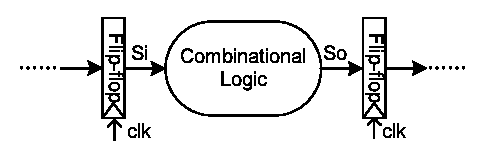
\includegraphics[width=0.5\textwidth]{fig2-1.eps}
  \vspace{-0.5em} 
  \caption{Generic logic circuit}
  \label{comb}
\end{figure}

The $S_i$ gets updated only at every effective clock transition and is held for the whole cycle period, which means almost no variable period exists. Thus the variable period, and the stable period of $S_i$ in the $n^{th}$ clock cycle $((n-1)T, nT)$ can be expressed as:
\begin{align}
%F_{s}^{S_i}&=f_{s_i}((n-1)T+t_{cq}) \label{Sivs}\\
T_{vp}^{S_i}&=((n-1)T, \;(n-1)T+t_{cq}), \\
T_{sp}^{S_i}&=((n-1)T +t_{cq}, \;nT).
\end{align}

The variable period of $S_o$, unlike that of $S_i$, is much more prominent; the $S_o$'s  variable period and stable period in the $n^{th}$ clock cycle can be expressed as:
 \begin{align}
%F_{s}^{S_o}&=f_{s_o}((n-1)T+t_{cq}+t_{pd})\\
T_{vp}^{S_o}&=((n-1)T+t_{cq}+t_{cd},\; (n-1)T+t_{cq}+t_{pd}) \\
T_{sp}^{S_o}&=((n-1)T+t_{cq}+t_{pd},\; nT+t_{cq}+t_{cd}) \label{SoSP}
\end{align}

Figure \ref{tvts} illustrates the time periods of both $S_i$ and $S_o$ in the $n^{th}$ cycle, where $t_{1}=(n-1)T+t_{cq}+t_{cd}$, $t_{2}=(n-1)T+t_{cq}+t_{pd}$.

\begin{figure}[ht]
\centering
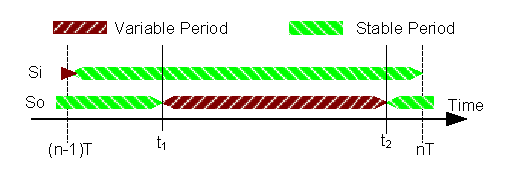
\includegraphics[width=0.65\textwidth]{fig2-2.eps}
   \vspace{-0.5em}
   \caption{Variable Period VS. Stable Period}
   \label{tvts}
\end{figure}

With the defined time periods, we can explain how the target faults commit the above violations and, what's more, how these IVV and TVV converge to SV.

1) Suppose that a delay fault occurs, the delayed $S_o$ will cause SV in Detection Slack ($T_{DS}$) during which the $S_o$ should keep stable. Equivalently, the delay fault will result in $S_o$'s TVV since at the end of the cycle, $S_o$ can not reach the expected value. This TVV then causes the IVV of the signal in the next stage of logic. Hence, SV, TVV, and IVV are equivalent to each other for the delay fault.

2) Suppose that an aging delay occurs, the delayed $S_o$ will cause SV in Guard Band ($T_{GB}$). Unlike the delay fault, the progressive aging delay will not cause TVV and IVV; therefore, an aging delay just represents as SV. Here the aging induced SV actually is quite similar to setup time violation.

3) Suppose that an unmasked SEU strikes the upstream flip-flop. Clearly, the $S_i$'s SV is committed because, after transient clock-to-q time, $S_i$ is supposed to keep stable during the whole cycle period. This SV could also potentially cause the downstream flip-flop to capture faulty data, and thereby results in $S_o$'s TVV, then IVV of input signals in the next stage logic. So, the SEU will represents as SV, and possible IVV and TVV.

4) Suppose that an unmasked SET happens in the combinational logic. If the duration of the SET is less than $T_{DS}+T_{GB}$, the behavior of the SET fault is similar with the commonly referred delay faults: unexpected signal transitions within the $S_o$'s stable period. Therefore, the analysis result for the delay faults also holds for SET faults. That is SV, TVV, and IVV are equivalently to each other for the SET.

From the above analysis we conclude that, from the signal behavior perspective, the target faults either induce equivalent SV, IVV, and TVV (for delay fault and SET), or only represent as SV (for aging delay), or SV and possible equivalent IVV and TVV (for SEU). In other words, the target faults can be uniformly modeled as SV. The implication is that we can employ a unified stability checker to handle the detection for all of the target faults. This unification can potentially support a more efficient implementation of the online fault detection scheme than the traditional redundancy-based approaches such as \cite{Mitra_C05}\cite{Han_DT05}. In addition, the capability for aging failure prediction \cite{failure_prediction_07}\cite{failure_prediction2_08} can be exploited in place with the same scheme; thereby greatly facilitating the aging-aware designs.

\subsection{Timing Constrains Exploration}
The object of SVFD in essence is to distinguish those transitions violating the signals' stability specification from normal signal transitions, thereby achieving the goal of fault detection. The detection of SV can be accomplished with some kind of stability checkers.

\subsubsection{Propagation of Stability Violation}
The stability checkers are usually implemented with dynamic circuit style. So, the first concern is how to schedule the precharge period. Neither the traditional cycle-begin precharge (using the first half cycle period to precharge) nor cycle-end precharge (using the second half cycle period to precharge) styles are applicable in our detection mechanism. As Section III.B explained, during the \emph{Guard Band} and \emph{Detection Slack}, the checker should be on duty, instead of staying in precharge state. Given $S_o$ with prominent variable period, the precharge can be scheduled in the variable period. However, the same schedule strategy is unallowable for $S_i$ because there is almost no any variable period can be exploited for precharge. If we "brutally" borrow some time from $S_i$'s stable period for precharging the checker, the fault coverage has to be sacrificed.

To address this problem, we find if the precharge stage is scheduled according to some specific timing requirements, the fault coverage will not be compromised. The discussion about timing manipulations can be started with describing a key observation, called {\bf Propagation of Stability Violation}.

Suppose that an unmasked SEU occurs in an upstream flip-flop at time $t$ in the $n^{th}$ cycle, then the effects of the SV of $S_i$ should be propagated to $S_o$ within the time interval of $(t+t_{cd},\;t+t_{pd})$.  If the effects of $S_i$'s SV can propagate into $S_o$'s stable period, that is

\begin{equation}\label{precharge}
(t+t_{cd},\;t+t_{pd}) \subset (nT-T_{GB}, nT+T_{DS}), 
\end{equation} 

Then the SEU induced $S_i$'s SV can be represented as $S_o$'s SV since the $S_o$ should keep stable during the \emph{Guard Band} and \emph{Detection Slack}. Hence, the checker deployed to detect $S_o$'s SV can indirectly handle a part of $S_i$'s SV within a particular time interval, referred to {\bf Propagation Detectable Period (PDP)}. From (\ref{precharge}), we have

\[
\left\{
\begin{array}{ll}
 t+t_{cd} > nT-T_{GB}, \\
 t+t_{pd} < nT+T_{DS}.
 \end{array} \right.
\]

Then, the PDP can be expressed as

\begin{equation} \label{eq2}
\{t\,|\, nT-T_{GB}-t_{cd} < t <nT+T_{DS}-t_{pd}\}.
\end{equation}

\subsubsection{XOR Protection}

Not all unmasked SEUs occurring in the upstream flip-flop can translate into the $S_o$'s SV; for example, if a  $S_i$'s SV happened during the $((n-1)T,\; t_1)$ (Figure \ref{tvts}), then it could not be detected by $S_o$'s checker  because (\ref{precharge}) dose not hold in such case.

To cover this period, one way is to set another stability checker for $S_i$, at the expense of almost doubled area and power overhead. In contrast, we propose a simple but far more efficient way to cover this period, referred to \emph{XOR Protection}, as Figure \ref{xor} shows. The effectiveness of this scheme is based on the observation: the $S_o^{(K-1)}$ is consistent with the $S_i^K$ within the period of $((n-1)T,\; (n-1)T+t_{cq}+t_{cd})$; therefore, one XOR (or NXOR) gate is capable of capturing any $S_i^K$ stability violation during this span of time. The overhead imposed by an XOR gate is much less than that imposed by another stability checker or other traditional redundant flip-flop based schemes \cite{Mitra_C05}. How to efficiently handle the output of XOR will be presented in next Section.

\begin{figure}[t]
\centering
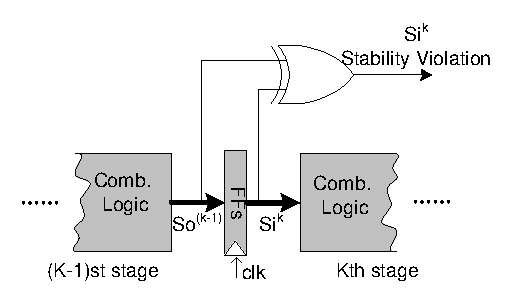
\includegraphics[width=0.45\textwidth]{fig2-3.eps}
\vspace{-0.5em}  
\caption{XOR Protection}\label{xor}
\end{figure}

\subsubsection{SEU Detection "Blind Zone"}

The above timing constrains are still not comprehensive without taking another time interval called "blind zone" into account.  Considering the propagation delay of a SEU, we can claim that the SEU must be benign if

\begin{equation}\label{benign}
t>nT-t_{cd}.
\end{equation}

\begin{figure}[ht]
\centering
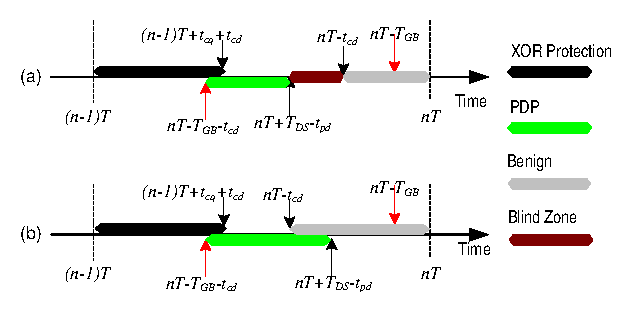
\includegraphics[width=0.75\textwidth]{fig2-4.eps}
  \caption{Variety of timing period for $S_i$}\label{zones}
\end{figure}

To protect $S_i$ (from SEUs), besides the XOR protection period, the PDP, and the benign period, there might be the fourth region that has not be covered so far. Figure \ref{zones} shows that the whole Stable Period of $S_i$ could be divided into four or three zones, depending on different timing parameters. Specifically, Figure \ref{zones}(a) shows if $nT+T_{DS}-t_{pd}<nT-t_{cd}$, then a SEU occurring in the interval of ($nT+T_{DS}-t_{pd},\;nT-t_{cd}$)  may fail to propagate into the detectable period, thereby resulting in detection "Blind Zone". Unlike the XOR protection period, this trouble can not be eliminated unless another dedicated stability checker is set for $S_i$, at considerable expense of implementation overhead. Fortunately, we propose a new approaches: Contamination Delay Optimization, by which the ``Blind Zone" can be eliminated by some timing manipulations.

\noindent{\bf Contamination Delay Optimization:} Clearly, the "Blind Zone" can be naturally
eliminated if

\begin{equation}\label{ebz}
nT-t_{cd} < nT+T_{DS}-t_{pd}
\end{equation}

is satisfied, as Figure \ref{zones}(b) illustrates. The SEU happening in $(nT-T_{GB}-t_{cd}, \; nT+T_{DS}-t_{pd})$ is either propagated into a Stability Violation detectable zone of corresponding $S_o$, or has nothing detrimental effect due to residing in benign period. From (\ref{ebz}), we derive the contamination delay should meet 

\begin{eqnarray}\label{eq80}
 t_{cd} > t_{pd} - T_{DS}
\end{eqnarray}

In addition, given that the terminal time of XOR protection zone should meet

\begin{equation}
  nT-T_{GB}-t_{cd} < (n-1)T + t_{cd} + t_{cq}; \nonumber
\end{equation}

otherwise another "blind zone" would emerge; thus, we have

\begin{equation}\label{eq81}
  t_{cd} > \frac{1}{2}(T-T_{GB}-t_{cq}).
\end{equation}

Lastly, considering  $T_{DS}<t_{cq}+t_{cd}$ should always holds, that is
\begin{equation}\label{111}
  t_{cd}>T_{DS}-t_{cq}.
\end{equation}

From (\ref{eq80}), (\ref{eq81}), and(\ref{111}), we derive that $t_{cd}$ should meet the requirement:

\begin{eqnarray}\label{eq82}
  t_{cd} >  \max \{t_{pd} - T_{DS},\; \frac{1}{2}(T-T_{GB}-t_{cq}),\; T_{DS}-t_{cq}\}
\end{eqnarray}

Generally, (\ref{eq82}) requires the contamination delay of the combinational logic reaches up to about a half cycle period. The same requirement is needed to be satisfied in some previous studies \cite{lowcost_date07} to address "short path effects" \cite{Nicolaidis_ITC07}. Actually, It is consistent with the goal of many timing optimization strategies \cite{Delay_Insertion_06}\cite{Padding_93}, and therefore not a substantial limitation.

\subsubsection{Available Precharge Period}
Figure \ref{zones}(b) sheds light on when the precharge can be scheduled: within $(nT-T_{GB}-t_{cd},\; nT-T_{GB})$ the precharge can be conducted without sacrificing fault coverage. Additionally, to avoid the precharge intruding Detection Slack, the actual available start point of the precharge stage should be

\begin{eqnarray}\label{eq5}
\max\{nT-T_{GB}-t_{cd},\;(n-1)T+T_{DS} \};
\end{eqnarray}

therefore, the available precharge period is

\begin{equation}\label{prechargeperiod}
(\max\{nT-T_{GB}-t_{cd},\;(n-1)T+T_{DS} \},\; nT-T_{GB}).
\end{equation}

From (\ref{prechargeperiod}), the available precharge duration $\tau$ can be calculated by

\[\label{tao}
\tau = \left\{
\begin{array}{ll}
 t_{cd} & \mbox{if } t_{cd}<T-T_{GB}-T_{DS}, \\
 T-T_{DS}-T_{GB} & \mbox{otherwise}.
 \end{array} \right.
\]

To sustain normal operations, there is a minimum precharge duration $\tau_0$, which is determined by the intrinsic $RC$ constant. Clearly, $\tau > \tau_0$ needs to be satisfied. It is not difficult to meet this requirement. Experimental results show that for 65nm CMOS, 1GHz, $\tau_0$ is merely 40ps, while $\tau$ is at the magnitude of hundreds of picoseconds. More detail can be found in next Section.

To sum up, we can use only one stability checker, with the assistant XOR protection, for soft errors, aging delay, and delay faults detection for $S_i$ and $S_o$. All we have to do is to ensure (\ref{eq82}) and (\ref{prechargeperiod}).

As the end of this section, the following exemplifies an empirical analysis of the above constrains.

\vspace{0.3cm} {\bf Example.} Generally, $T_{DS}$ is determined by the maximum width of SET pulses, commonly conservatively being set to a half cycle period, that is $T_{DS}=0.5\times T$. $T_{GB}$ originally is determined by the aging detection interval---the time interval between two aging detection action (the aging sensor does not need to be always on).  $T_{GB}$ is much larger than 5\% of cycle period, as suggested by \cite{failure_prediction_07}, but should be less (or not much larger) than the reserved timing margin. Since commonly 10\% timing margin is reserved to combat PVT variations, the cycle period dose not need to be increased to reserve extra time margin for $T_{GB}$. The propagation delay $t_{pd}$ hence is $T\times(1-10\%)=0.9T$. We omit the term of $t_{cq}$ because comparing with other timing parameters, $t_{cq}$ is marginal. Then, based on (\ref{eq82}) we need to figure out the minimal $t_{cd}$ since smaller $t_{cd}$ implies that smaller compensation effort and associated area overhead to pay. We suggest use the results: $t_{cd}=0.45T$, $T_{DS} = 0.45T$, $T_{GB}=0.09T$ because this configuration is competent enough in detecting SET faults, delay faults, and aging delays with modest compensation effort.

\subsection{On-line Fault Detection Architecture}
Figure \ref{imple}(a) shows the top view  of the whole fault detection scheme. Note that the XOR (NXOR actually) output needs to be gated outside of the XOR protection period where an XOR-flagged alarm can unintentionally discharge the detection unit if leave un-gated. The detailed timing relations and associate clock configurations is shown in Figure \ref{imple}(b), where CLKS is used to control precharge-evaluation, and CLKG is the gating clock for XOR output.

\begin{figure}[t]
\centering 
\subfigure[Top view of SVFD scheme]
{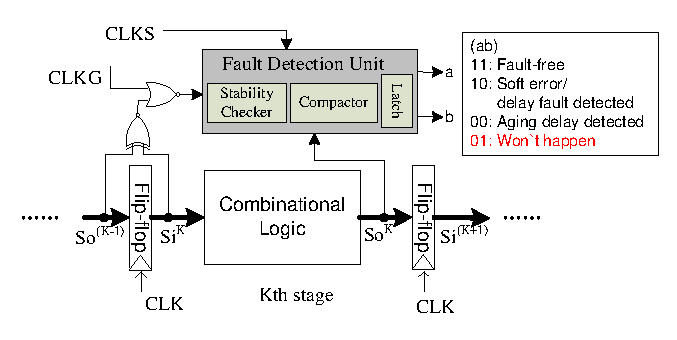
\includegraphics[width=0.6\textwidth]{fig2-5a.eps}} 

\subfigure[Timing of precharge clock and XOR-protection gating clock]
{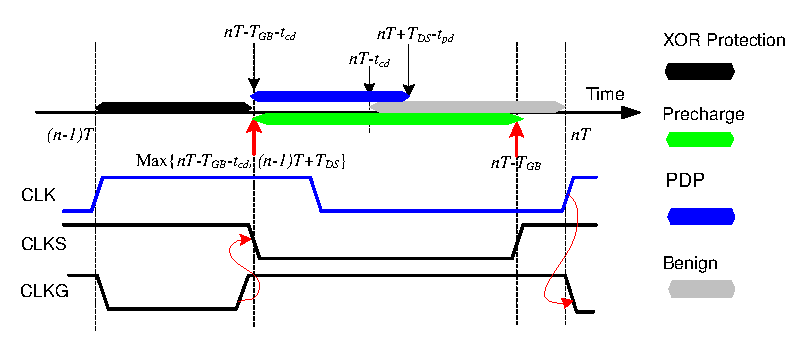
\includegraphics[width=0.7\textwidth]{fig2-5b.eps}}  \caption{Top view of implementation}
\label{imple}
\end{figure}

\subsubsection{Circuit Design}
Figure \ref{circuit} shows the transistor level design of SVFD scheme. A detection unit consists of two key components: a stability checker (Figure \ref{circuit}(b)) and an output compactor (Figure \ref{circuit}(c)).

\begin{figure}[t]
\centering
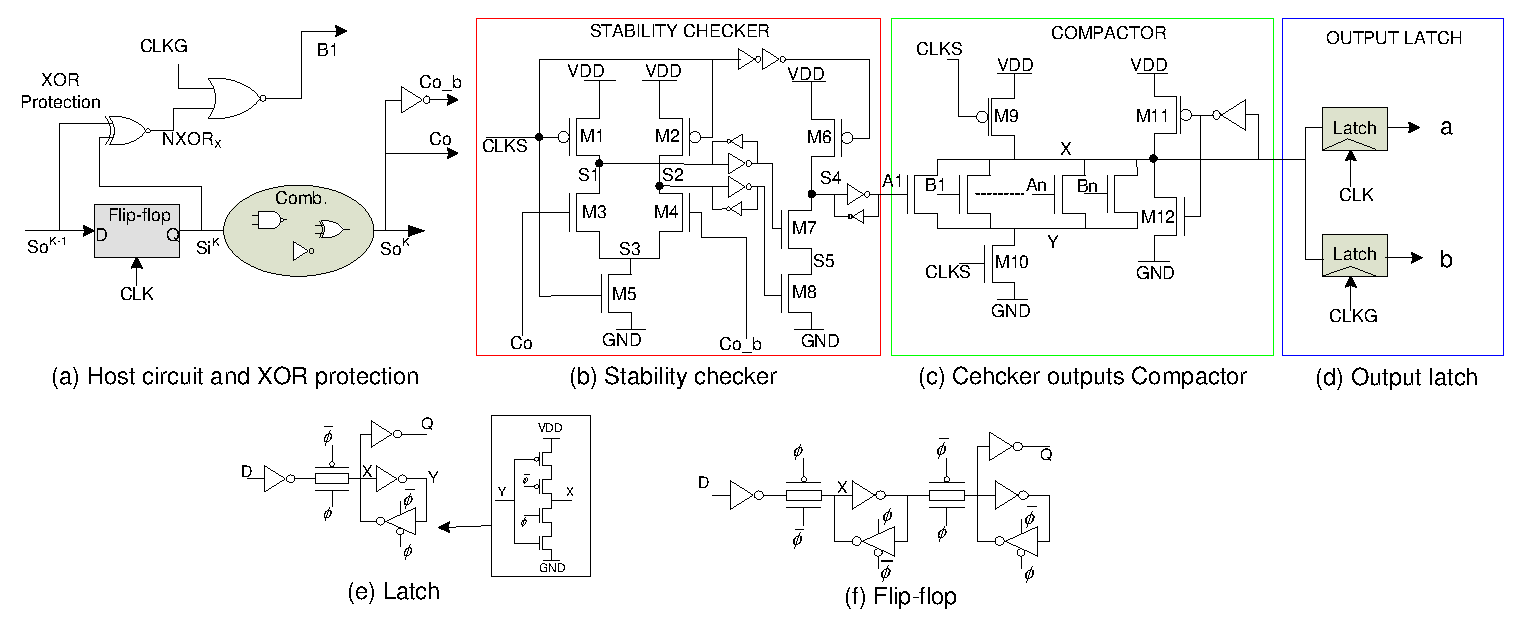
\includegraphics[width=0.95\textwidth]{fig2-6.eps}
\vspace{-0.5em}  
\caption{SVFD Implementation} \label{circuit}
\end{figure}

The basic stability checker can be derived from a sensing circuit for on-line delay fault detection \cite{sensing_96}, in which the signal integrity is verified by a pair of consistent charge/discharge nodes, a delay fault will trigger one of the nodes to be discharged/chargeed and thereby causes states inconsistent between them. The same fundamental detection principle is employed to design a sensor dedicated for aging prediction, referred as Aging Resistant Stability Checker (ARSC) \cite{failure_prediction_07}. Based on the same principle, we design a new stability checker. Compared with ARSC, the checker has several new features which can improve the robustness and reduce the overhead. The following explains how does the circuit work and then presents the new features.

During precharge period, both nodes $S1$ and $S2$ in the stability checker are charged up to HIGH. Then, the circuit starts evaluation, one of the two nodes is pulled down, while the other one floats at HIGH because the gate signal of M3 is always complemented with that of M4 (a weak keeper can help the floated node stick to HIGH). Hence, the node $S1$ and $S2$ are always exclusive during fault-free time, which will make the node $S4$ stick to HIGH because the high-impedance path between S4 and GND always exists. When a Stability Violation is committed by $S_i$ (out of the XOR protection period) or $S_o$, the violation will trigger the discharge of the node that has charged up to HIGH. Eventually both nodes are discharged, and thereby the node S4 is pull down to LOW. Then, the node X in output compactor will be discharged, which flags a fault being detected. The compacted result X needs to be latched twice: CLK-latched for indicating aging delay and CLKG-latched for indicating soft error or delay fault (Figure \ref{circuit}(d)). The reason will be explained in Section VIII.

\begin{figure}[t]
\centering \subfigure[XOR Tree] {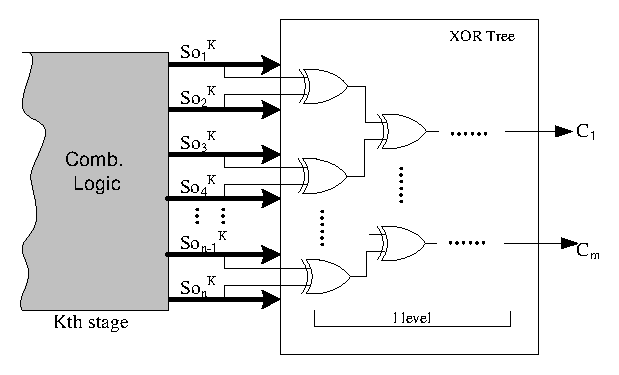
\includegraphics[width=0.4\textwidth, height=0.25\textwidth]{fig2-7a.eps}}
\hspace{1cm} \subfigure[AND Tree]
{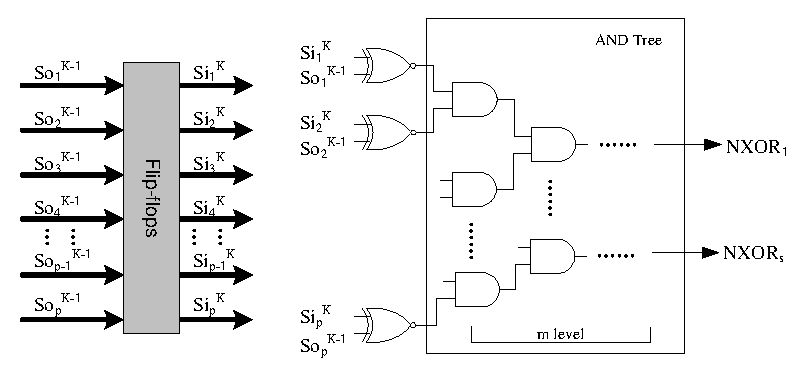
\includegraphics[width=0.53\textwidth,height=0.25\textwidth]{fig2-7b.eps}}  \caption{Compacting the
output signals and XOR-protection signals} \label{compactor}
\end{figure}


There are two new features in the detection unit:

1) The NOR logic for combining the states of S1 and S2 is realized with a dynamic
logic (M6, M7, and M8), which can improve the robustness of the checker and reduce
the area overhead and switch power dissipation. Unlike the stability checker in ARSC
\cite{failure_prediction_07}, where the checker output, a static NOR gate, is
directly driven by a floated HIGH node during fault-free time, our checker's output
is generated by a dynamic NAND gate. This change is based on that both the node S1
and S2 are pulled up to HIGH during precharge, and consequently both M7 and M8 are
turned off; thereby no short path existing when precharge. So the foot transistor
for the dynamic NAND is eliminated. Note that due to the precharge RC delay of S1
and S2, the M6's precharge clock should be delayed by a precharge delay constant to
avoid transient shot current in the NAND gate.

2) The outputs are compacted with a dynamic NOR for reducing the number of output
latches. Usually, it is not necessary to identify which signals commits the SV for
most aging-aware and fault tolerant designs. So the distributed detection results
can be ``compacted" to reduce the number of output latches. We use a wide dynamic
NOR to implement the compactor, in which the M11 and M12 serve as a level restorer
for node X.

%The fault detection is for providing fail-stop support or some on-line adjustments. While, so far,
%the fault detection can detected the fault at fine-grained: signal. This grained of fault
%detection is unnecessary, especial in the situation where the chips have been shipped to the
%customers.

%In addition,
%%this detection unit can be easily disabled by pulling up the CLKS to HIGH. The PMOS
%%transistor's aging process induced by NBTI effects is greatly slow down in disable
%%mode.
%unlink ARSC where the Guard Band is confined by a clock and its delayed counterpart
%\cite{failure_prediction_07}, SVFD unit provides Guard Band by the  CLK and CLKS. So
%the clock skew needs to be controlled well. This issue is beyond the scope of this
%paper.


\subsubsection{Low-Overhead Deployment}
Given a target circuit, each output signal $S_o$ needs to be monitored by a
stability checker whose output is fed to a compactor, as Figure \ref{imple}(a)
shows. In addition, each XOR-protected signal gated by CLKG is also fed to a
compactor.   We present two deploying techniques to reduce the overhead coming from
the checkers, compactors, and latches.

\textbf{Compacting $S_o$ using XOR-Trees:} With XOR-Trees, we can enable checker-sharing mechanism among multiple output
signals, as Figure \ref{compactor}(a) shows, thereby reducing the number of
checkers. The rationale behind the XOR-Trees based compactor is the fact that for a XOR gate the non-simultaneous transitions of inputs can result in output transitions. This can be explained with the following example:

Suppose there are two signals $S_a$ and $S_b$, and signal $C = S_a \mbox{XOR} S_b$;
clearly, one or two non-simultaneous transitions of $S_a$ and $S_b$ can be exactly represented as or or two transitions of $C$. This fact implies that if $S_a$ or $S_b$ imposes stability violations, then $C$ must commit stability violations, too.

One side effect of XOR-Trees is that the compactor may hide some faults that happen to induce simultaneous transitions on the primary inputs of a XOR-Tree. For example, if $S_a$ happens to switch from HIGH to LOW, while at the same time $S_b$ from LOW to HIGH, then  $C$ may keep staying at HIGH. Fortunately, the possibility of such negative cancelation effect can be minimized by separating the $S_o$ from the same logic cone to different XOR-Trees, since it is rare for multiple faults happen in the same spot at the same time, especially for soft errors.

Figure \ref{compactor}(a) illustrates an application of a set of XOR-Trees which compacts $n$ output signals $So_1^K, So_2^K,\ldots, So_n^K$ into $m$ checker-monitored signals $C_1, C_2, \ldots, C_m$. We have 

\begin{equation}
m=\frac{n}{2^{\,l}}.
\end{equation}

The number of required XOR-gate used to implement an XOR-Tree can be easily calculated by

\begin{equation}\label{nxor}
  N_{xor}=n\times (1-(1/2)^{\,l}).
\end{equation}

%\begin{figure}[t]
%\centering
%\includegraphics[width=0.4\textwidth]{xortree.eps}
% \caption{XOR Tree}\label{xortree}
%\end{figure}

\textbf{Compacting $S_i$  using AND-Trees:} The similar strategy can be used to compact the XOR-protection results with AND-Trees. If one or more SEUs strike the set of flip-flops, then corresponding inputs of the set of AND-Trees will be pulled down to LOW, and then pull down the outputs of corresponding AND-Trees, denoted by NXORx in Figure \ref{compactor}(b).

Unlike XOR-Trees for compacting output signals, AND-Trees won't suffer form the cancelation effect because one or more SEUs yield the same effect: pulling down the corresponding AND-Tree's output to LOW.

With the two deployment optimizations, we can derive the number of required checkers $N_{checker}$, compactors $N_{compactor}$, and output latches $N_{latch}$. Suppose for a circuit with $n$ flip-flops, $l$-level XOR-Trees and $m$-level AND-Trees are employed, then we have

\begin{equation}\label{nchecker}
  N_{checker} = \frac{n}{2^{\,l}};
\end{equation}

\begin{equation}\label{ncompactor}
  N_{compactor} = \frac{n}{BW}( \frac{1} {2^{\,m}}+\frac{1}{2^{\,l}}),
\end{equation}

where $BW$ (bandwidth) is the number of input signals of a compactor;

\begin{equation}\label{nlatch}
  N_{latch} = 2 N_{compactor}.
\end{equation}

\textbf{Timing implication of XOR-Trees and AND-Trees:} The delay implication of the AND-Tree and XOR-Tree should be considered. The CLKG has to be postponed to accommodate the delay of the AND-Tree, denoted by $t_{and}$. The CLKS should also be postponed by the delay of $\mbox{min}\{t_{and}, t_{xor}\}$, where $t_{xor}$ denotes the delay of the XOR-Tree. The impact of the two delays is the increased detection latency. In the worst-case, the detection unit needs extra $\mbox{max}\{t_{and}, t_{xor}\}$ time to complete, but this increase in latency will not substantially impair the effectiveness of the fault detection as long as output latch time is also postponed accordingly. Specifically, the first latch's clock CLK (Note, not the main flip-flop clock) is delayed by $\mbox{max}\{t_{and}, t_{xor}\}$ and the second latch's clock CLKG by $t_{and}$.

Of course, one should also keep the delay of the AND-Trees and XOR-Trees from being the new critical paths in the target circuit. The empirical analysis of delay can be achieved based on classical logic effort theory \cite{Logic_effort}. Empirically, given a $m$-level AND-tree (each logic gate is two-input), the path logic effort is $(4/3)^m$; the path electric effort is $5/4$ because the load of the output signal is only a NOR gate. Then the path effort is $(4/3)^m\times 5/4$. The path parasitic delay is $2m$.  Hence, the minimum delay $D_{and\_min}$ can be given by

\begin{equation}\label{anddelay}
  D_{and\_min}=m\times ((4/3)^m\times 5/4)^{1/m} + 2m
\end{equation}

Based on  (\ref{anddelay}), we find the optimized AND-Tree delay is a quasi-linear function of $m$. For a 3-level AND-Tree, the delay is about 2 Fo4, even for a up to 10-level AND-Tree, the delay does not exceed 7 Fo4.

For an XOR-Tree with the same levels, the minimum delay $D_{xor\_min}$ is about $3 D_{and\_min}$ because the logic effort for an XOR gate is three times larger than that of an XOR gate \cite{Logic_effort}. Therefore, the delay constraint on the XOR-Trees will be much stringent than that on the AND-Trees. Given the 10$\backsim$18 Fo4 clock period of today's pipelined processors \cite{Victor_TC04}, for example, the maximum level of each XOR-Tree should be no more than four levels.


A major drawback to adopting such AND-Trees and XOR-Trees is the degraded detection resolution---when a checker flag an alarm, we can not precisely identity the fault spot in the target circuit because  the AND-Trees and XOR-Trees can exponentially expend the "region-under-control" of a specified fault detection unit. However, this issue is trivial since we only focus on efficient fault detection---which serves as the primary step for most backward error recovery schemes. 

\subsubsection{Clock Variation Consideration}
The delayed clocks can be generated from locally delaying the system clock CLK, as prior work \cite{failure_prediction_07} did, or obtained from a DLL. To ease the implementation worry, the following cites some industry data to show that generating the clocks with well-defined intentional skew should not be a substantial problem. DLLs have been widely used to reduce the clock skew across clock domains \cite{clock_01}\cite{DLL_00}\cite{DLL2_04}. The detailed design of a DLL is beyond the scope of this paper. Many industry practices have shown that implementing clocks with only 10-picosecond skew is practical. For example, even in conventional tree-based clock networks across $500mm^2$ processor die with frequency up to 2.5GHz , the unintended clock skew can be efficiently limited to less than 10ps \cite{Itanium_clock05}. While previous study \cite{failure_prediction_07} shows that a reasonable $T_{GB}$ is usually around 100ps for a 1GHz system. Therefore, generating the CLK, CLKS, and CLKG with well-defined intentional skew should not be a substantial problem. The sophisticated variation-resilient clocking scheme is beyond the scope of this paper.

Another practice, Razor II \cite{Razor2_ISSCC08}, can also back up the feasibility of clocks used in SVFD.  Razor II also relies on strict clocks. An auxiliary clock, called DC, is employed. The deployment of CLKG in our SVFD scheme is not harder than that of DC in Razor II scheme. Hence, we believe that implementing the supportive clocks is practical.


\begin{figure}
\centering
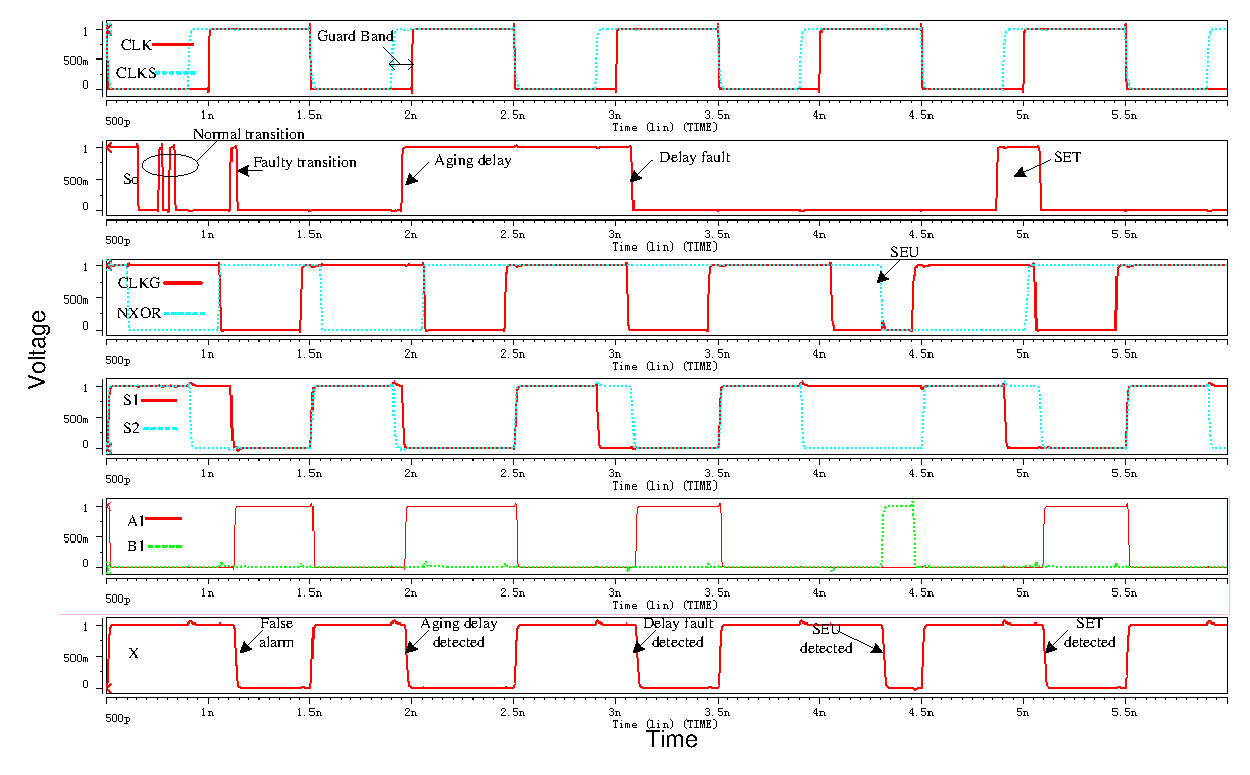
\includegraphics[width=0.99\textwidth, height=0.6\textwidth]{fig2-8.eps}
\caption{Hspice simulated signal state transitions}\label{spice}
\end{figure}


\subsection{Experiment Result Analysis}
The experiments consist of two parts. The first is dedicated for evaluating a basic fault detection unit in terms of detailed timing verification, area overhead, power, and performance. The results are obtained by using the Hspice targeting the next-generation 32nm Predictive Technology Model \cite{PTM_06} for High-performance applications.  The second shows an application to a fully pipelined floating-point unit (FPU), with emphasis on analysis of chip-level area and power overhead and comparisons with other solutions.

\begin{table}[t]
\begin{center}
\caption{Comparing Tradeoffs with other schemes}\label{comparison1}
\begin{tabular}{l||ccccc}
 {\bf Overhead}     &  SEFF\cite{Mitra_C05}  &  LOWCOST\cite{lowcost_date07} &  ARSC\cite{failure_prediction_07}  &  CWSPFF\cite{CWSP_DATE08}    &  SVFD \\
\hline
Transistor          & 14     & 36       & 24     & 46       &  36   \\
Power               & 1.00      & $>$1.00        & $>$0.10$^\triangleleft$   &  N/A     &  1.16  \\
performance         & 0      & N/A      & $<$1\% & $<$1\%   &  $<$1\%\\
Clock               & 1      &  2       &  2     & 2        &  3    \\
\hline
\hline
  {\bf Applicability}     & Limited$^\diamond$ & Limited &  General & General & General \\
\hline \multicolumn{6}{l}{N/A:  Not applicable.}\\
\multicolumn{6}{l}{$\diamond$  The scheme needs support from a specific scannable flip-flop.}\\
\multicolumn{6}{l}{$\triangleleft$  ARSC uses a different metric of power overhead.} \\

\end{tabular}
\end{center}
\end{table}


\subsubsection{Evaluating SVFD Unit}
Figure \ref{spice} shows the detail timing of a SVFD unit in consecutive five cycles. The topmost shows the system clock CLK, the precharge-evaluation clock CLKS, with which the guard-band defined. The second shows the monitored signals $S_o$. The third illustrates the XOR-protection signal and corresponding gating clock. The fourth shows the state transitions of the two most important internal node S1 and S2. The fifth shows the signals A1---the output of the stability checker, and B1---the gated output of XOR protection unit. Both are feeded to the same compactor.The bottom most shows the detection result generated by the compactor.

During the first cycle (0---1ns), $S_o$ presents some normal transitions. In the first half of the second cycle (1---1.5ns), an unexpected glitch, which is supposed to simulate a benign SET fault, occurs; then in the guard band of the second cycle, an aging delay is simulated. A delay fault is simulated in the third cycle. In the fourth cycle, a SEU fault is simulated by pulling down the NXOR signal.

From the bottom figure, we can see that all the SV shown in the second and third waveforms are successfully detected, represented by LOW state of node X.

We zoom in the figure to extract some useful timing information (the zoomed figures are omitted due to space limitation): 1)the critical precharge time $\tau_0$ is about 40ps, while the available precharge time is about 400ps---one order of magnitude larger than $\tau_0$. Hence, the precharge time will not be a limitation when we manipulate the related timings. 2)The detection delay is just about 40ps which is merely 2 Fo4 delay in 32nm technology. 3)The maximum undetectable glitch width is about 18ps, which is even less than most soft error induce glitch width in 32nm technology, so the robustness of SET detection should not be in question.

Table \ref{comparison1} shows the tradeoff comparisons between SEFF \cite{Mitra_C05}, LOWCOST \cite{lowcost_date07}, ARSC \cite{failure_prediction_07}, CSWPFF \cite{CWSP_DATE08}, and SVFD. we use the number of transistors as the area overhead metric, as many circuit-level studies adopted.

To conduct comparisons between variety schemes, a baseline latch and flip-flop design needs to be determined. Figure \ref{circuit}(e) and (f) show the adopted baseline design. The similar latch design is used by Intel as a standard datapath latch \cite{Latch_01}. The flip-flops is used in PowerPC603 processor \cite{Flipflop_94}. In addition, an XOR gate consumes at least 12 transistors when computing the number of transistors (eight transistors for the core XOR logic and another four for generating the inverter versions of input signals). For fairness, only the checker and its input generating logics are considered; the subcomponents that can be shared among checkers (i.e. output compactor, and output latches) are not taken into account though such amortization will make the area overhead of SVFD more attractive.

{\bf Area:} As Table \ref{comparison1} indicates, SEFF is most economic scheme in term of area overhead; however, this benefit has to be based on a dedicated scannable flip-flop design in which each functional flip-flop has a replica, called shadow flip-flop,  to support scan test. This heavy reliance on the specific scannable flip-flop, though greatly facilitate an area-efficient design, limits the applicability of SEFF, since not all designs use the same design-for-test techniques and implementation. LOWCOST can be regarded as a mutation of SEFF, but with a delay between the functional flip-flops and its' shadow counterpart. Thus, LOWCOST face the same issue of limited applicability. Clearly, if the shadow flip-flops are treated as overhead transistors, then the total transistors overhead must be much higher than that shown in table \ref{comparison1}.

{\bf Power:} We use a relative power penalty $R_p$ to evaluate the power:

\begin{equation}
  R_p=\frac{\mbox{Power of a detection unit}}{\mbox{Power of a flip-flop}}.
\end{equation}

We compare the power of the detection unit against that of a standard flip-flop, respectively, with the same input signal and frequency. The input signal changes value every cycle. The Hspice results show that the stability checker is relatively power-hungry---16\% higher than the power of a flip-flop.  This is mainly because the checker is implemented with dynamic circuit style. The Compactor logic, however, is much power-saving---a 8-input compactor only consumes 40\% power of a flip-flop; this because when fault-free, all input signals fed to a compactor won't discharge it. The power of output latches even drop to only 10\% of a flip-flop because there no state transition happens to the latch during fault-free state, thus no dynamic power consumed.

As for other solutions,  SEFF's power is doubled ($R_p=1$), as \cite{Mitra_C05} shows, since a redundancy flip-flop is enabled. Similar modification is conducted in LOWCOST, and moreover an extra lath is employed; hence the power of LOWCOST must be slightly larger than that of SEFF ($R_p>1$).

Note that our checker seems much more power-hungry than ARSC. That is because the power overhead metric in \cite{failure_prediction_07} is different with ours. In ARSC, the power overhead is calculated as the whole logic (include both the flip-flop and combinational logic) power increase. Because the combinational logic's power is relatively constant, so the actual sensor power consumption compared with a flip-flop should be much higher.

{\bf Performance:} The performance mainly depends on the flip-flops time overhead and the critical path delay. In SVFD, there is no modification to the flip-flops and the critical path is not changed as well. The only timing penalty results from several extra gate capacitances drived by the $S_i$ and $S_o$. Our experiment result shows this penalty is less than 1\% for a special combinational logic: 8-inverter chain.  In fact, the other SEFF, LOWCOST, ARSC, and CWSPFF face the same situation, but no one get hurt from it.

{\bf Clock:} We compare the number of clock (phase) used by these schemes. For example, SEFF dose not need any extra clock; LOWCOST, ARSC, CWSPFF, need one extra clock skewed with respect to the system clock. while SVFD needs two extra clocks: CLKS and CLKG. This is a negative attribute of SVFD since the extra clocks could potentially increase the complexity; as a tradeoff, however, the SVFD's detection capability is the most versatile over the other four schemes.

{\bf Applicability:} The SEFF and LOWCOST need the support from a particular type of scannable flip-flop, but the other three schemes do not suffer from this limit.

\subsubsection{Case Study---An application of SVFD}

We use a case study to demonstrate the main considerations when deploying SVFD, with emphasizing on area and power implications.

The pipelined FPU adopted by OpenSPARC T1 \cite{OpenSPARC_06} is used as our target circuit which implements the SPARC V9 floating-point instructions and supports all IEEE 754 floating-point data types. The FPU comprises three independent pipelines: Multiplier pipeline (MUL), Adder pipeline (ADD) and Divider pipeline (DIV). More design details can be found in \cite{OpenSPARC_06}.

The FPU was synthesized using Synopsys Design Compiler with UMC 0.18um technology, with performance as the synthesizing priority.

\vspace{0.3cm} \noindent{\bf Experimental Setup}

First, several timing parameters are determined. Specifically,
\begin{itemize}
  \item The cycle period $T$ is defined according to $t_{pd}$; given 10\% margin reserved,   $T={10}/{9}\times t_{pd}$. The critical path delay ($t_{pd}$) reported by PrimeTime is $1.7ns$, so $T=1.87$ns.

  \item The clock-to-q time $t_{cq}$ depends heavily on a specific flip-flop design and technology. Given 180nm technology for the design in Figure \ref{circuit}(f),  $t_{cq}$ is about 110 ps; Thus, we get $t_{cq} = 0.06T$.

  \item  Next, $t_{cd}$, $T_DS$, and $T_{GB}$ needs to be determined. We prefer minimize $t_{cd}$ since larger $t_{cd}$ implies more path compensation area needed to pay, while check whether $T_{DS}$ and $T_{GB}$ meets the common requirement, for example, $T_{DS}\approx0.5T$ and $T_{GB}>0.05T$ \cite{lowcost_date07} \cite{failure_prediction_07}. From (\ref{eq82}), we figure out the minimal $t_{cd}$ is 0.79ns ($0.43T$), at which $T_{GB}=0.095T$, $T_{DS}=0.48T$. Then, we check out that $T_{GB}$ indeed meets the requirement: larger than $0.05T$ while less than timing margin ($0.1T$). $T_{DS}$, however, is slightly smaller than $0.5T$; considering such minor mismatch won't impose any substantial problem for delay fault and SET detection, we prefer to keep $T_{DS}=0.48$ while paying the minimal path compensation overhead.
\end{itemize}

Second, at RTL-level, we integrated parts of the SVFD infrastructure---the XOR-Protection, XOR-Trees, AND-Trees---into the target FPU. It is difficult to integrate corresponding stability checkers and compactors because these logic are highly custom dynamic logic at transistor-level; however, since we focus on overhead evaluation, so this difficulty can also be resolved in an "indirect" way. The area overhead imposed by these dynamic logic is estimated based on the data in Table \ref{comparison1}. The short-path compensation is realized by imposing a timing constraints when conducting RTL synthesis. After the compensation process, we conduct the post-simulation to verify pipelines functionality and timing.

Third, we use PrimePower (a gate-level power simulation and analysis tool provided by Synopsys for power evaluation. The modified FPU are exercised with random input operands for 100,000 cycle, at the same time, dump the according VCD (Value Change Dump) format data for power evaluation. The power of checkers and compactors are still evaluated with Hspice. We wrote a C++ program to convert the output of the XOR-Trees and AND-Trees (VCD format) into PWL voltage sources which are recognizable for Hspice version checker and compactor to conduct a transistor-level power evaluation. Then, the Hspice-reported power is scaled to fit PrimePower-reported power based on $R_p$, thereby obtaining the overall power consumption.

\begin{figure}
\centering 
\subfigure[Area overhead and associated overhead breakdown] {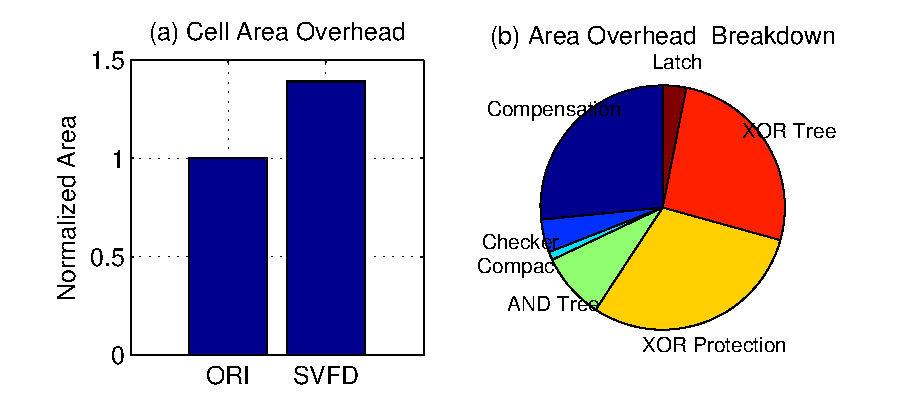
\includegraphics[width=0.7\textwidth]{fig2-9a.eps}} 
\subfigure[Power overhead and associated overhead breakdown] {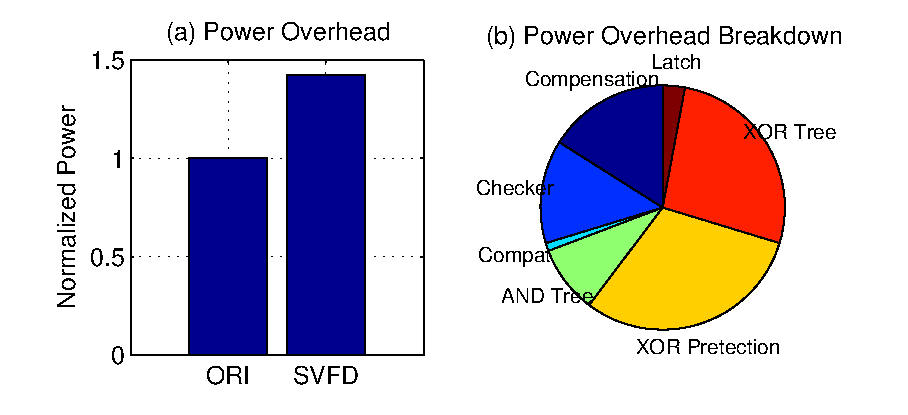
\includegraphics[width=0.7\textwidth]{fig2-9b.eps}}
\caption{Area and power with configuration: $L_{xor}=3$, $L_{and}=3$, $BW=8$.} \label{area_power}
\end{figure}

\begin{figure}
\centering \subfigure[Implication of $L_{xor}$ and $L_{and}$ on area overhead]
{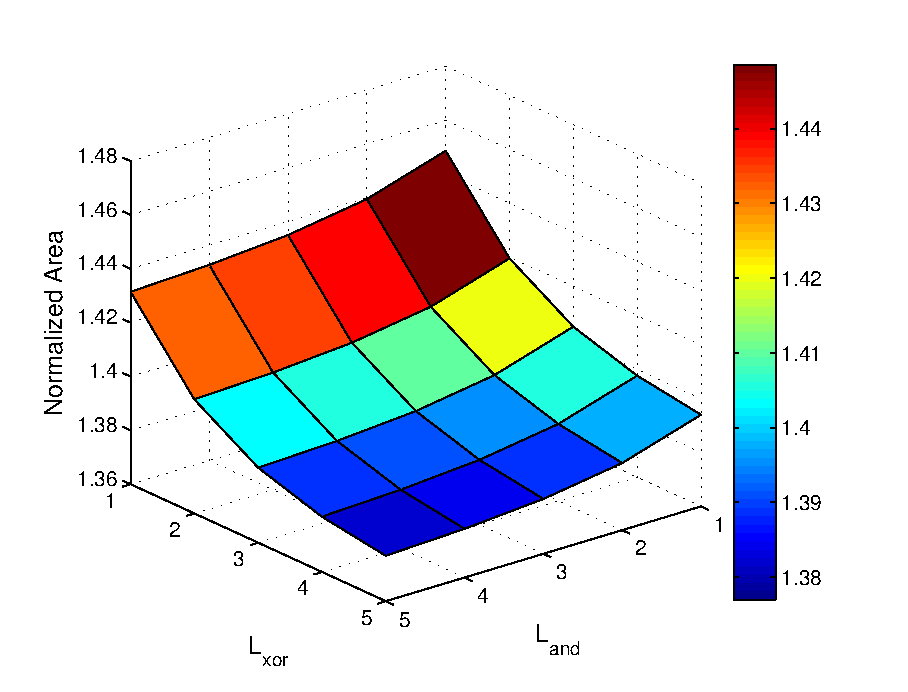
\includegraphics[width=0.45\textwidth, height=0.35\textwidth]{fig2-10a.eps}}  \subfigure[Implication of
$L_{xor}$ and $L_{and}$ on power overhead]
{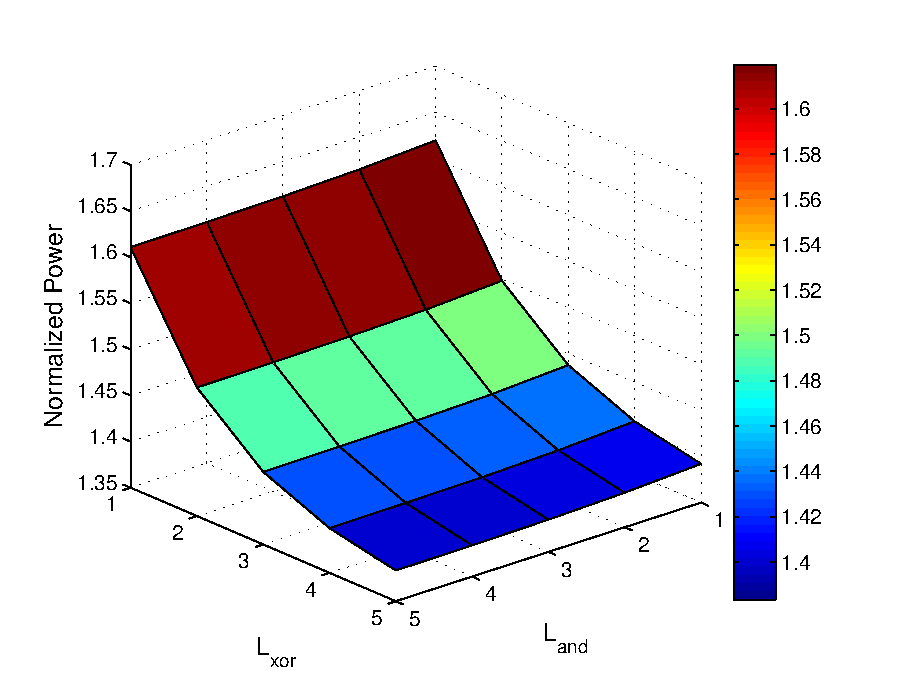
\includegraphics[width=0.45\textwidth, height=0.35\textwidth]{fig2-10b.eps}} \caption{Implication of
$L_{xor}$ and $L_{and}$ on area and power, $BW=8$.} \label{lxor_land}
\end{figure}

\vspace{0.3cm}\noindent{\bf Experimental Results}
The configurable parameters are 1) the level of XOR-Tree ($L_{xor}$), 2) the level of AND-Tree ($L_{and}$), and 3) the bandwidth of the compactor ($BW$). We first study the overhead at the tentative configuration: $L_{xor}=3$, $L_{and}=3$, $BW=8$, and then seek to optimize it. Figure \ref{area_power} shows the corresponding experimental results.

Figure \ref{area_power}(a) compares the SVFD's area, denoted by SVFD, against that of the original FPU, denoted by ORI. The total cell area overhead is about 40\%. This overhead comes from 1) compensating the short path to meet the $t_{cd}$ requirement, 2) the stability checkers and associated compactors  and latches, 3) the AND-Trees and XOR-Trees, and 4) the XOR-gates for XOR protection. Among these breakdowns of area overhead, “ompensation" and ”XOR Protection" are constant for a given target circuit because the former is determined by the minimal contamination delay and the later by the number of flip-flops; however, the other portions are configuration-specific. The corresponding power implication is shown in Figure \ref{area_power}(b). The overall power overhead is 43\%. In addition, two significant implications, which can guide to a more efficient configuration, can be drawn from these results:
\begin{enumerate}
  \item  The checker's area and power are unproportionate:  4\% area overhead   contributing to 14\% power penalty. Hence, reducing the number of checkers should   be an effective way to optimize the  overall power penalty.

  \item  Increasing the $BW$ of compactors has very marginal benefit to reducing the overall area and power since the area and power of the compactors and associated output latches together take only 4\% and 3\%, respectively.
\end{enumerate}

One way to reduce the number of checkers is to adopt the XOR-Trees with higher levels. The same strategy can be considered to optimize the overhead imposed by AND-Trees. Figure \ref{lxor_land} shows the overhead trends with different $L_{xor}$ and $L_{and}$ configurations.

The first perception gained from this figure is the power issue is much more crucial than the area issue: the worst-case power penalty can reach up to 1.62$\times$ while the area is only 1.45$\times$. In addition, the headroom for area optimization is limited comparing with that of power optimization. Hence, prioritizing the power optimization should be much effective for reaching an optimum design tradeoff. In SVFD scheme, power optimization actually does not conflict with area optimization.

Second, both the area and power trends are more sensitive to $L_{xor}$ than to $L_{and}$. In particular, as Figure \ref{lxor_land}(b) shows, the impact of $L_{and}$ to the power is almost negligible. Note that although increasing $L_{xor}$ and $L_{and}$ seems facilitate more area- and power-efficient deployment, we should keep the delay implication of the XOR-Tree and AND-Tree in mind (Section V.C). For the pipelined FPU implemented with 180nm technology, the $T$ is about 17 Fo4 ($\approx 1.9ns/110ps$). We suggest configuring the XOR-Tree with fours levels, and the AND-Tree with five levels. With this configuration, the following will compare SVFD with several recently proposed solutions from cell area and power aspects.

\begin{figure*}[!t]
\centering \subfigure[] {
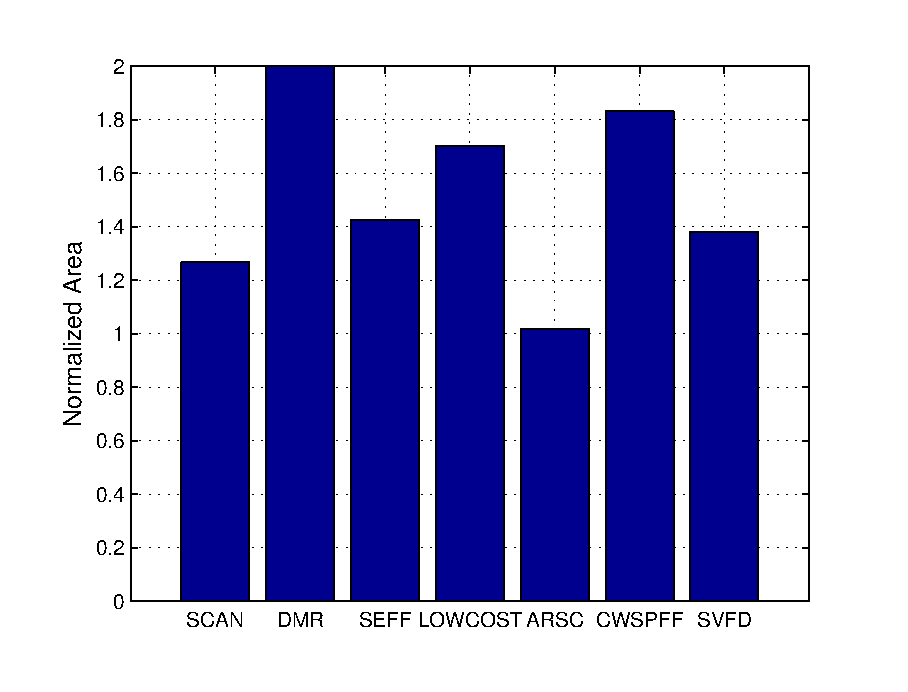
\includegraphics[width=0.4\textwidth, height=0.3\textwidth]{fig2-11a.eps}}\subfigure[] {
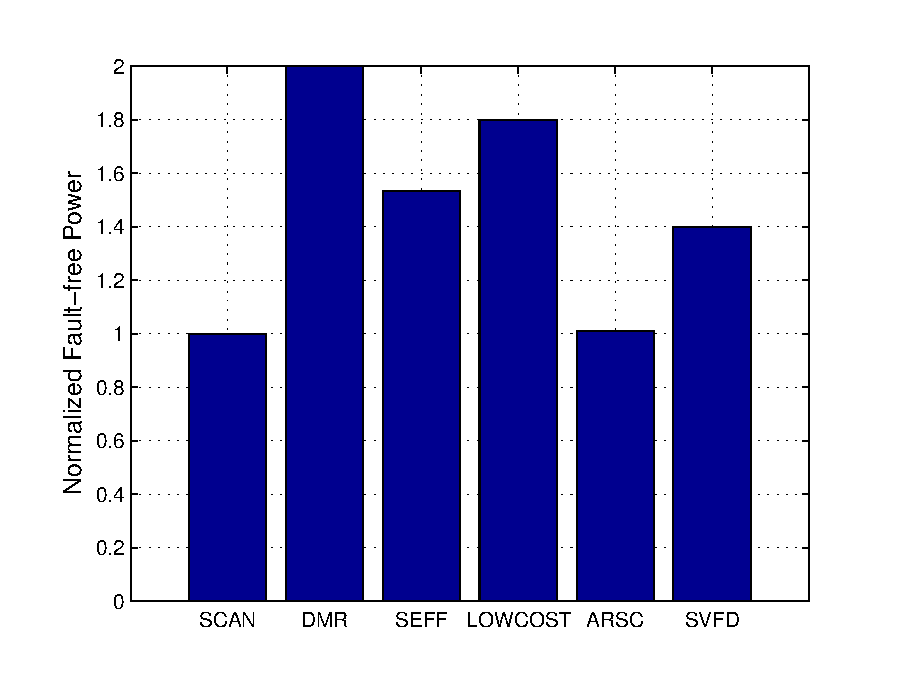
\includegraphics[width=0.4\textwidth, height=0.3\textwidth]{fig2-11b.eps}}
\caption{Comparison with other solutions in terms of cell area and power,
$L_{xor}=4$, $L_{and}=5$, $BW=8$.} \label{APcomparison}
\end{figure*}

\subsubsection{Comparison with other schemes}
Figure \ref{APcomparison} gives the comparison results. SCAN denotes the scannable version of the original pipeline. In SCAN, all pipeline flip-flops are substituted by a scannable flip-flops in \cite{Mitra_C05}. DMR represents the traditional dual-module-redundancy (we simply double the original area and power to show DMR's overhead implication. In fact, for any meaningful DMR, other synchronous overhead such as output comparison should be also imposed). SEFF is implemented by substituting the scannable flip-flops for a self-checking flip-flops \cite{Mitra_C05}. LOWCOST is substitute the scannable flip-flops with another modified flip-flops in which the clock of shadow flip-flop is skewed from that of the functional flip-flops; in addition, an output latch is also inserted \cite{lowcost_date07}. CWSPFF is also based on a slightly modified DFF and additional Equivalence checker, another shared logic whose overhead can be amortized by the other logics \cite{CWSP_DATE08}, but even we neglect the amortizable logics, we believe that this solution is also not overhead-economic, given the results indicated in Table \ref{comparison1}. ARSC is dedicated for only aging delay detection \cite{failure_prediction_07}.

Figure \ref{APcomparison} (a) shows different total cell area required to deploy these solutions. In which, ARSC presets to be the most area-economic, this mainly because the ARSC logic only need to be deployed in the timing critical portions in terms of aging delay detection. The same reason, combined with the fact that the ARSC logic does not need to be always-on, makes the chip-level power overhead of ARSC negligible \cite{failure_prediction_07}, as "ARSC" bar in Figure \ref{APcomparison} (b) shows.

We bar SCAN in Figure \ref{APcomparison} is not because it can facilitate some fault detection or recovery (actually it incapable for any fault detection), but it can be viewed as the foundation of SEFF and LOWCOST.

Figure \ref{APcomparison} shows that the overhead imposed by SVFD is very comparable with that of other schemes: the area overhead is 39\%, and the power penalty is 40\%---both are superior to that of SEFF scheme, while SEFF can only handle SEU faults. Given that SVFD can cope with SEUs, SETs, delay faults, aging delays; therefore, we conclude that the versatile SVFD is more promising.

Note that we omit the CWSPFF's power implication in Figure \ref{APcomparison} is because re-implement this scheme in our target pipeline is very labor-intensive and time-consuming. But considering the complexity of the CWSPFF logic and associated deployment, the power overhead should not superior than that of SEFF. In addition, compared with SVFD's versatile capability, CWSPFF can only handle SET faults.

%All of the above analysis is with respect to the ORI circuit. If we switch to with
%respect to the SCAN, the area overhead of SVFD will decrease and the power
%effectiveness of SVFD differs little.

\begin{table}[t]
\begin{center}
\caption{Comparison of detection capability }\label{comparison}
%\begin{tabular}{l|p{0.8cm}p{1.5cm}p{1cm}p{1.2cm}p{0.6cm}}
%\extrarowheight=1pt \tabcolsep=2pt
\begin{tabular}{l||ccccc}
    &  SEFF\cite{Mitra_C05}  &  LOWCOST\cite{lowcost_date07} &  ARSC\cite{failure_prediction_07}  &  CWSPFF\cite{CWSP_DATE08}    &  SVFD \\
\hline
%\multicolumn{6}{c}{}\\

            SEU        &  Yes   & Yes    & No     & No     & Yes  \\
            SET        &  No    & Yes    & No     & No     & Yes  \\
            Aging delay&  No    & No     & Yes    & No     & Yes  \\
            Delay fault&  No    & Yes    &  No    & Yes    & Yes  \\
\hline %\multicolumn{6}{l}{'---' :  Aging delay does not need any recovery routine.}\\
 %\multicolumn{6}{l}{'90\%':  fault coverage for SEU is $(1-0.095T/T)\approx 90\%$.}\\
\end{tabular}
\end{center}
\end{table}

\subsection{Discussion}
\subsubsection{On SVFD Application}
With the increasing impacts of soft errors and transistor aging under the relentless CMOS scaling, we believe SVFD will be increasingly promising. In part is because SVFD is far more area efficient than traditional DMR based schemes, in part for its versatile capability for fault detection. But SVFD does not suppose to totally take the place of existing approaches, especially ECC based schemes.  The following will discuss how to apply SVFD efficiently and why SVFD is a significant complement to existing schemes.

Modern processor includes two types of structures: logic-dominated structures such as execution units and memory-dominated structures such as register file, caches \cite{Revival_08}. Using  SVFD for logic-dominated structures, as the FPU in our experimental study, are cost-efficient. Since such type of structures usually are so non-regular that engineers mostly have to resort to coarse-grained DMR, thereby imposing more area and power overhead. Moreover, the SVFD can also indicate the aging process, which is an essential benefit that the traditional DMR can hardly achieve.

As for protecting the regular memory-dominated structures from in particular soft errors, ECC has been proven to be a highly cost-effective approach. SVFD can not beat ECC in terms power and area overhead, though SVFD can also detected soft errors in memory-dominated structures since soft errors induced perturbations can also results in stability violation in primary outputs. The prior research shows that, with extensive architectural hits such as register lifetime prediction \cite{Using_Register_Lifetime_dsn07}, selective placement \cite{Exploiting_selective_placement_taco08}, ECC-based approach commonly dictates about 30\% area overhead. This overhead is comparable with that of SVFD. While one ECC's benefit that SVFD does not possess is error correction---the commonly used ECC is able to correct single-bit fault and detect two-bit fault. Hence, we think ECC is still the preferred option for memory-dominated structures in a microprocessor.

But SVFD scheme offers aging prediction that ECC-based doesn't. The aging process of SRAM cells exhibits by increased read-out and write-into delay. The read delay is more critical than write delay because the read path usually serves as the critical path \cite{Mitigating_Parameter_Variation_micro07}. While for the SVFD sensors the degraded read operations behave the same with the degrade critical delay in logics, and hence can also be handled by a simplified SVFD sensors that are only for aging prediction---as Agarwal et al. proposed previously \cite{failure_prediction_07}.

Hence, we conclude that SVFD is a cost-efficient application for protection logic-dominated structures; combined with ECC based approaches which can already handle soft errors, SVFD can also provided additional capability for aging prediction for memory-dominated structures.

\subsubsection{Variation and Aging Considerations}
Just as DMR cannot be free from false positive, SVFD face the same situation. The systematic variation hurts little to SVFD unit as well as other fault detection infrastructures because it statistically exhibits distinct spatial locality and correlation. If the SVFD suffers from the systematic variation, so does the host circuits in the same silicon spots. But random variation in some corner cases can invalid the SVFD unit. As shown in Figure \ref{circuit}, for example, if the leakage of M3 is overly large due to random variation, and at the same time the keeper for S1 happens to be too weak to compensate the escaped charge through M3, then a false alarm will be flagged. In other words, if S1's keeper does not happen to be that weak, the SVFD unit is highly probable to work. The same situation comes to M4. Therefore, on one hand, these keepers can help cancel out part of negative effects of random variation; on the other hand, we can properly size the transistors on the discharge paths to obtain more robustness against random process variation.

As the transistors in host circuits, the transistors in the SVFD unit also wear out over time. While the other hardware-based fault detection schemes such as LOWCOST and DMR suffer from the same situation. But the core logics, i.e. stability checker (Figure \ref{circuit}(b)) and compactor (Figure \ref{circuit}(c)) are relatively resistant to NBTI---one of the major aging mechanisms, because all of the PMOS transistors in the two logics are timing non-critical, while all the timing critical transistors are NMOS transistors which intrinsically are free from NBTI. Hence, we believe SVFD units have good chance to stand longer than the host circuits due to the better NBTI resilient characteristics.



\subsubsection{Distinguish Detection Results}
It is useful to  distinguish the aging delay caused detection positive from the rest of detection results,  because the detected aging delay rate is used as the input for some aging-aware designs.

SVFD implicitly apply a rule for distinguish the detected results. That is: If a stability violation is detected in Guard Band, then this violation is viewed as aging delay induced; the stability violation detected in other region is viewed as soft error or delay fault induced. Figure \ref{circuit}(d) is used to implement this rule. However, this might degrade the confidence level of detected aging delay rate since if a stability violation takes place within the Guard Band, SVFD can not determine whether this violation is caused by a soft error or an aging delay.

Fortunately, this confidence degradation incurred by this implementation is negligible. To quantitatively evaluate the miss rate, we define the miss as: a soft error induced stability violation is misjudged as an aging-fault stability violation.

Suppose that the raw soft error rate (SER), $R_{soft error}$, is uniformly distributed over time. The detectable SER is $\alpha R_{softerror}$, where the $\alpha$ is a constant ($0<\alpha<1$) related to the three masking effects \cite{Shivakumar_DSN02}. The aging fault rate is denoted as $R_{aging}$.

The misjudgment rate $R_{miss}$ can be expressed as
\begin{eqnarray}\nonumber
R_{miss}&=&1-\frac{R_{aging}}{R_{aging} + \alpha R_{soft error}\times\frac{T_{GB}}{T_{DS}+T_{GB}}}
\end{eqnarray}

Practically, the Guard Band should not be larger than the timing margin to avoid extra timing penalty. A typical timing margin is 10\%. Assume that $\alpha=0.5$, and $R_{soft error} =0.1\times R_{aging}$ (actually, after some detectable aging effects of devices begin emerging, the assumptions of $\alpha$ and raw SER are heavily conservative ), $T_{GB}/T_{DS}=0.2$ then $R_{miss}$ is not large than 1\%. Therefore, we can safely conclude that the imperfect distinguishing capability will not impose any substantial problem.

\section{On-Chip Path Delay Measurement}
In this paper, we present a novel on-chip path delay measurement architecture for efficiently detecting and debugging of delay faults in the fabricated integrated circuits. Several delay stages are employed in the proposed on-chip path delay measurement (OCDM) circuit, whose delay ranges are increased by a factor of two gradually from the last to the first delay stage. Thus, the proposed OCDM circuit can achieve a large delaymeasurement range with a small quantity of delay stages. A calibration circuit is incorporated into the proposed on-chip path delay measurement technique to calibrate the delay range of the delay stage under process variations. In addition, delay calibration for import lines is conducted to improve the precision of path delaymeasurement. Experimental results are presented to validate the proposed path delay measurement architecture.

\subsection{Path Delay Measurement and Fault Tolerance}
    With the scaling of semiconductor process technology, the performance of modern VLSI chips improves significantly. We have seen operating frequencies of integrated circuits reach multi-gigahertz, resulting in more rigorous timing requirements \cite{ITRS09} \cite{zeitzoff2002mosfet}. Timing related defects originated from manufacturing process-related problems, such as resistive opens and shorts, metal mouse bites, via voids, etc., will become more common \cite{hawkins2003view}. Consequently, delay faults caused by these physical defects, which prevent the circuit from meeting the timing requirements, are of growing concern in nanometer technologies \cite{krstic1998delay}. Moreover, it should be noted that the manufacturing process is becoming more difficult to be controlled with the increasing complexity of modern VLSI chips. Therefore, electrical parameters, such as saturation current, gate capacitance, threshold voltage, etc., may vary from one device to another. As a result, the delay of gates and timing-critical paths will have large variations and can hardly be predicted during the design stage due to the imprecision of verification models \cite{blaauw2008statistical} \cite{agarwal2003statistical}. Furthermore, the circuit timing would also be impacted by the application environment conditions such as temperature, supply voltage noise, etc. In order to improve the quality of shippable products, there is an urgent need to conduct effective delay testing for ascertaining the correct operation of chips at the rated frequency \cite{mak2004new} \cite{krstic1998delay}.

\subsubsection{Challenges for Path Delay Measurement}
Traditionally, at-speed delay testing is implemented to check the satisfiability of circuit timing by only considering whether the circuit under test (CUT) passes delay testing under the applied test vector pairs or not. However, under the process and environment variations, it requires to test the chip at different worst case timing scenarios to ensure the circuit’s timing correctness \cite{krstic2001delay} \cite{zhang2008multiple} \cite{fu2008robust}. For example, for a circuit path with a very small slack, even though it passes a test under the at-speed test clock frequency, it possibly fails another test that induces larger capacitive coupling or power supply noise.

The small delay defect (SDD), which introduces only a small extra delay over its normal value, may fail to be detected by at-speed delay testing due to the observability limitation for a large timing slack. However, the detection for SDDs is increasingly important to ensure the chip’s quality and reliability \cite{menon2009output} \cite{ahmed2006novel}. The first important reason is that a timing failure can be occurred in the circuit during functional application caused by the increment of small delay on paths with small timing slacks \cite{kruseman2004hazard}. The second important reason is that the SDDs hidden in the circuit may become one of the major reliability limiters \cite{nigh2000test} \cite{tayade2008small}. In addition to the imperative requirement for SDD detection, it is well known that in order to improve the yield and reduce the time-to-market of chips, design-related failures and performance limiters need to be identified and rectified as early as possible during first silicon debug \cite{balachandran2002facilitating}. However, it is very expensive to use external high-speed automatic test equipment (ATE) for post-silicon debug of modern high-performance chips. Moreover, the frequency of test clock generated by external ATE would be affected by factors such as parasitic capacitance, resistance of probe and tester skew, etc. \cite{sunter1998bist}. In addition, for a complex system-on-chip (SOC), the internal circuit modules are limited to be accessed by the external ATE to conduct silicon debug.

The on-chip path delay measurement techniques have been gained many attentions for researchers in recent years, for it can provide a cost-effective alternative way to perform delay defect detection and silicon debug in modern VLSI chips. Rather than testing the chip with all possible worst-case test vectors and process corners, it is better to measure the delays of paths and to check if the slacks are large enough to tolerate all the possible delay variations. Therefore, high complexity for finding the worst case test vectors considering different sources of variations can be avoided and high test confidence can be obtained. Moreover, by on-chip measuring the delays of selected paths in the actual silicon, precise path timing information can then be obtained for circuit under actual operating conditions. As a result, whether there are SDDs on a path can be analyzed based on the measured path delay. Further, the amount of timing violations in the failing paths can be obtained under certain environment conditions \cite{datta2004delay} \cite{ datta2006scheme}. Valuable information, which points the performance limiter and source to circuit failure, can hence be obtained by the on-chip path delay measurement technique with a much higher confidence.

\subsubsection{Prior Path Delay Measurements}
Several on-chip architectures have already been proposed for delay testing and silicon debug in literatures. Ghosh et al. \cite{ghosh2006novel} presented a built-in delay-sensing circuit to improve the delay fault coverage of the CUT. The delay of the path under test is converted to a certain voltage height by using a saw-tooth waveform generated from the reference clock signal. By comparing the converted voltage with the reference voltage, delay fault of the target path can then be detected. The same technique is also used in \cite{raychowdhury2005novel} for speed binning of the high performance chips based on the delay measurement results for circuit’s critical paths. Hsiao et al. \cite{tayade2008chip} proposed a built-in parametric measurement circuit for time-interval measurement based on the dual-slop technique. The capacitor is first charged by the input voltage with a high slope, and then the capacitor is discharged with a known lower slope. Therefore, the time-interval can be derived from the discharging time based on the proportional relationship between the discharging time and input voltage. Wang et al. \cite{wang2008path} proposed a ring oscillator based scheme for path delay measurement. By configuring the path under measurement (PUM) and the returning loop into a ring oscillator, delay of the target path can be translated into oscillation period. Tayade et al. \cite{tayade2008chip} utilize a programmable capture generator to obtain a fast capture signal to conduct faster-than-at-speed testing. Small delay defects can then be efficiently detected by this approach. Moreover, delays of the selected paths in circuit can also be measured by sweeping the capture clock frequency. Datta et al. \cite{datta2006scheme} proposed an on-chip timing characterization scheme based on the skewed inverter delay line. First a pulse is generated by the triggered transitions of the start and end points of the PUM using the test vector, and then the width of pulse is recorded into the latching circuits by using pulse shaping technique. Datta et al. \cite{datta2004chip} proposed a modified vernier delay line (VDL) technique for path delay measurement. By using a balanced delay line, high-resolution capability for delay measurement can be provided. Based on the same principle of VDL technique, the delay scan chain is proposed in \cite{datta2004delay} to reuse the existing scan chain for path delay measurement. Tsai et al. \cite{tsai2008all} proposed a built-in delay measurement circuit consisting of coarse and fine blocks, which is an extension of the modified VDL technique. However, the above VDL based techniques require lots of delay stages to achieve a large measurement range \cite{pei2009low}. Moreover, the delays of the import lines, which connect the chosen PUM into the path delay measurement unit, are not considered, thereby posing a significant influence on the precision of path delay measurement.

\subsection{Path Delay Measurement Circuits}
In this section, we present the design of OCDM for path delay testing and silicon debug. As mentioned above, the previous VDL based delay measurement techniques need lots of stages to achieve a large delay measurement range under the pre-determined delay measurement resolution. Consequently, the goal of the proposed OCDM circuit is to reduce the number of delay stages in the VDL, thus to achieve a significantly less hardware overhead as well as less delay measurement time.

\subsubsection{Basic Structure and Operation}
The basic structure of the proposed OCDM circuit is shown in Figure \ref{fig:OCDM-fig1}, which can convert the path delay of the PUM into a series of digital values that can be stored in the flip-flops of the VDL chain. Each delay stage consisted in the VDL chain is constructed by a positive edge triggered D-type flip-flop, four multiplexes, and several buffers. In the proposed OCDM circuit, we assumed that the input $x$ is fed by the output of the PUM, while the input $y$ is fed by the input of the PUM. So $y$ always switches earlier than $x$ does during the delaymeasurement period. In order to explain the operation of the OCDM circuit, let’s consider the case that both the input and output signals of the PUM are rising transitions.

\begin{figure}[t]
\centering
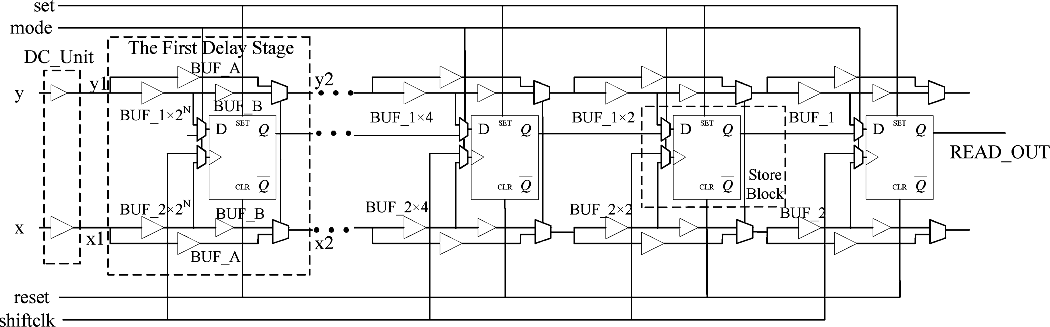
\includegraphics[width=0.85\textwidth]{OCDM-fig1}
   \caption{Proposed On-Chip Delay Measurement Circuit}
    \label{fig:OCDM-fig1}
\end{figure}


The upper delay unit (UDU) refers to the buffer chain that starts at the input of the delay stage at which the transition signal is propagated from node $y$, and ends at the input of the multiplexer whose output is connected to the data input of the flip-flop in each delay stage of the OCDM circuit. The lower delay unit (LDU) is similar to UDU, except that it starts at the input of the delay stage at which the transition signal is propagated from node $x$, and ends at the input of another multiplexer whose output is connected to the clock input of the flip-flop in each delay stage.

The delay range is defined as the delay difference between the two delay units in each delay stage of the OCDM circuit. For example, in the last stage of the OCDM circuit, the delay of UDU (named BUF\_1), $D_{buf\_1}$, is designed larger than that of LDU (named BUF\_2), $D_{buf\_2}$. Thus, the delay range of the last stage, $R_{last}$, is the delay difference between $D_{buf\_1}$ and $D_{buf\_2}$, i.e.,

\begin{equation} \label{eq:rlast}
    R_{last} = D_{buf\_1} - D_{buf\_2}.
\end{equation}

From the last stage to the first stage of the OCDM circuit, the delay range of each stage is increased by a factor of two. The DC\_Unit cell, as shown in Figure \ref{fig:OCDM-fig1}, is used for delay compensation, and will be explained in detail later. Two rising input transitions from the PUM pass through the DC\_Unit firstly, and then go into the inputs of the first delay stage of the OCDM circuit, respectively.

Let us explain the function of each delay stage by considering the operation of the first delay stage for the sake of clarity for illustration without loss of generality. Suppose the input and output signals of the upper delay chain in the first delay stage are $y1$ and $y2$, respectively, accordingly, $x1$ and $x2$ are assumed for the lower delay chain. All flip-flops of the OCDM circuit are initialized to logic ZERO values by asserting the reset signal. The delay measurementmode is activated by asserting the mode signal. As $x1$ and $y1$ signals propagate through their respective delay units, the time difference between the two signals will be reduced. As shown in Figure \ref{fig:OCDM-fig2}(a), assuming that $x1$ signal lags the $y1$ signal by enough time (i.e., $y1$ switches much earlier), and hence a logic-high value will be hold in the flip-flop. As a result, $y2$ will be the signal that passes through the UDU and the buffer BUF\_B in the upper delay chain from $y1$, while $x2$ will be the signal that passes through the LDU and the buffer BUF\_B in the lower delay chain from $x1$. The delay of BUF\_B is large enough to ensure that a stable logic high value can be stored in the flip-flop before the two transition signals arrive at the inputs of the multiplexers whose outputs are connected to the inputs of the next delay stage. Clearly, the time difference between $x2$ and $y2$ is reduced by an amount which equals the delay range of this delay stage.
\begin{figure}[t]
\centering
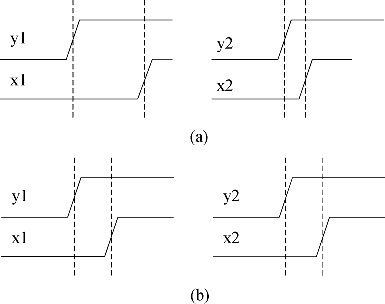
\includegraphics[width=0.85\textwidth]{OCDM-fig2}
    \caption{Relation between time difference of two input signals($x1$, $y1$) and that of two output signals ($x2$, $y2$) in the first delay stage. (a) Logic ONE in the flip-flop. (b) Logic ZERO in the flip-flop.}
    \label{fig:OCDM-fig2}
\end{figure}


The buffer named BUF\_A in each delay stage has a delay value that is larger than the cumulative delay of the path that contains LDU and BUF\_B of the same delay stage. Likewise, if the time difference of $y1$ and $x1$ is smaller than the delay range, the flip-flop will hold a logic ZERO value. Therefore, the signals propagating through BUF\_A are then selected by the multiplexers. As a result, the time difference between $y2$ and $x2$ will be equal to that of $y1$ and $x1$, as shown in Figure \ref{fig:OCDM-fig2}(b).

Consequently, the principle of the OCDM circuit is that if the time difference between the two inputs of each delay stage is lager than the delay range of the same stage, a logic ONE value will be stored in the flip-flop of the delay stage. The time difference between the two output signals will be updated by simply subtracting the delay range from that between the input signals of the delay stage. Otherwise, the flip-flop of the delay stage will hold a logic ZERO value, and the time difference between the output signals will keep the same as that between the input signals of the delay stage.


Note that there exists a setup time in the store block of each delay stage as shown in Figure \ref{fig:OCDM-fig2}, which consists of a D flip-flop and two multiplexers. If the time difference between the two inputs of the store block is smaller than the setup time (about 33ps in the experiment of this paper), an error logic value may be hold in the flip-flop. Therefore, in order to provide better delay measurement precision, the DC\_Unit cell constructed by two buffer lines is proposed for delay compensation, which means that the upper and lower delay units of DC\_Unit are designed such that the delay difference between them is approximately equal to the setup time. Meanwhile, if half of the delay range in the last delay stage is also compensated in the delay difference of the upper and lower delay units of DC\_Unit cell, the OCDM circuit can improve the delay measurement resolution by 50\%. The values stored in the delay line can be shifted out serially using the clock signal shiftclk in the shift mode by de-asserting the mode signal. The delay of the PUM can then be obtained.

\subsection{Delay Range Calibration}
The delay range of each delay stage in the OCDM circuit would be varied due to the prominent process variations. It is thus necessary to calibrate the delay ranges to assure the precision of path delay measurement result before using the OCDM circuit \cite{blaauw2008statistical} \cite{agarwal2003statistical} \cite{tsai2008all} \cite{datta2006scheme}. Figure \ref{fig:OCDM-fig3} shows the basic structure of the calibration circuit \cite{tsai2008all} \cite{datta2006scheme}, which can be embedded into the OCDM circuit for delay range calibration. The outputs of the calibration circuit, denoted as $y$ and $x$, are directly connected to the inputs with the same notations of the OCDM circuit, respectively.

\begin{figure}[t]
\centering
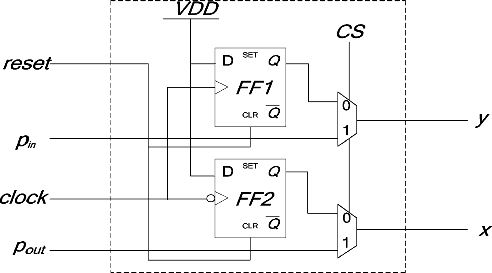
\includegraphics[width=0.65\textwidth]{OCDM-fig3}
   \caption{Calibration Circuit}
    \label{fig:OCDM-fig3}
\end{figure}


Two inputs of the calibration circuit, denoted as $P_{in}$ and $P_{out}$, are fed by the input and output of the PUM, respectively. Clearly, when the CS signal is set to 1, the generated transitions at the $P_{in}$ and $P_{out}$ can be sent into the OCDM circuit for delay measurement. When the CS signal is set to 0, the delay range calibration process is conducted.

The simplified timing waveform for the delay range calibration is shown in Figure \ref{fig:OCDM-fig4}. The FF1 and FF2 are rising and falling edge triggered flip-flops respectively. First, the flip-flops of FF1 and FF2 are initiated with logic ZERO by the reset signal. Then, logic ONE will be loaded into the FF1 and FF2 by the rising and falling edges of the clock signal respectively. Clearly, the time difference between the generated rising transitions at $y$ and $x$ is equal to the width of the positive half cycle of the clock signal. The time period of the clock signal can be programmed deterministically with high resolution using the on-chip clock generator from \cite{kaeriyama20071}.

\begin{figure}[t]
\centering
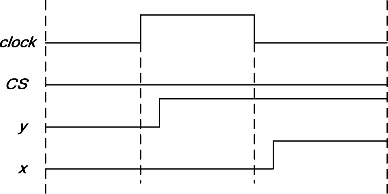
\includegraphics[width=0.65\textwidth]{OCDM-fig4}
   \caption{Simplified timing waveform for calibration circuit.}
    \label{fig:OCDM-fig4}
\end{figure}


Assuming the number of delay stages in the OCDM circuit is $m$. The following presents the calculation method for obtaining the delay range of each delay stage, which is described by Equation \ref{eq:eq-array}:
\begin{equation} \label{eq:eq-array}
    \begin{cases}
        a_{11}x_{1} + a_{12}x_{2} + ... +a_{1m}x_{m}=b_{1} \\
        a_{21}x_{1} + a_{22}x_{2} + ... +a_{2m}x_{m}=b_{2} \\
        ... \\
        a_{m1}x_{1} + a_{m2}x_{2} + ... +a_{mm}x_{m}=b_{m} \\
    \end{cases}
\end{equation}

Let

\begin{equation}
    A=
    \left[
    \begin{array}
        {cccc}
        a_{11} & a_{12} & ... & a_{1m}\\
        a_{21} & a_{22} & ... & a_{2m}\\
        ... & & & \\
        a_{m1} & a_{m2} & ... & a_{mm}\\
    \end{array}
    \right]
\end{equation}

\begin{equation}
    X=
    \left[
    \begin{array}
        {c}
        x_{1} \\
        x_{2} \\
        ... \\
        x_{m} \\
    \end{array}
    \right]
\end{equation}

\begin{equation}
    B=
    \left[
    \begin{array}
        {c}
        b_{1} \\
        b_{2} \\
        ... \\
        b_{m} \\
    \end{array}
    \right]
\end{equation}


The we can get Equation \ref{eq:array-abbr}.
\begin{equation} \label{eq:array-abbr}
    AX=B
\end{equation}

where $x_{j} \in (1 \leq j \leq m)$ in vector X represents the delay range of the $j$th delay stage to be calculated, $b_{i} \in (1 \leq i \leq m)$ in vector $B$ represents the width of the positive half cycle of signal clock for the $i$th calibration process, $a_{ij}$ in  matrix $A$ represents the measured value (0 or 1) for the $j$th delay stage during the $i$th calibration. Clearly, by selecting appropriate values for vector $B$ in each calibration process, it is easy to conclude the delay range for each stage by solving Equation \ref{eq:array-abbr}.

For example, assuming there are four delay stages in the OCDM circuit and we know their nominal designed delay ranges. After we choose 70, 55, 40, and 25 for $b_{i}$ in four calibration processes respectively, the obtained values for matrix A is listed as follows:

\begin{equation}
    A=\left[
        \begin{array}
            {cccc}
            1 & 1 & 1 & 0 \\
            1 & 0 & 1 & 1 \\
            1 & 0 & 0 & 0 \\
            0 & 1 & 0 & 1 \\
        \end{array}
        \right]
\end{equation}

Hence, after solving Equation \ref{eq:array-abbr}, the delay ranges are found to be 40, 20, 10, and 5 from the first to the last stage, respectively.

Note that the value of $b_{i}$ in the vector $B$, which is the width of the positive half cycle of the clock signal, may not be exactly equal to the expected value because of the clock jitter, and hence may induce error delay ranges for the delay stages. However, this can be compensated by multiple calibrations under each value because the clock jitter is a zero-mean random variable \cite{jan2003digital}. 

For example, if for the second calibration process is set to 55, the values in the second row of matrix $A$ are then expected to be equal to (1, 0, 1, 1) respectively. This can be represented by Equation \ref{eq:sum}.

\begin{equation} \label{eq:sum}
    55 = x_{1} + x_{3} + x_{4}
\end{equation}

However, if the width of the positive half cycle of the clock signal is varied from the expected value and is 50 or 60 due to the clock jitter, then the second row of matrix will get (1, 0, 1, 0) or (1, 1, 0, 0), respectively. Hence, the second row of matrix is replaced to Equation \ref{eq:sum13} or Equation \ref{eq:sum12} as follows:

\begin{equation} \label{eq:sum13}
    55 = x_{1} + x_{3}
\end{equation}

\begin{equation} \label{eq:sum12}
    55 = x_{1} + x_{2}
\end{equation}


Therefore, error values would be calculated for the delay ranges of the delay stages by using Equation \ref{eq:sum13} or Equation \ref{eq:sum12}. However, since the clock jitter is a zero-mean random variable \cite{jan2003digital}, we can calibrate the delay ranges using the same expected $b_{i}$ value for multiple calibration times. Though neither Equation \ref{eq:sum13} nor Equation \ref{eq:sum12} can be used to obtain the delay ranges correctly, the sum of the expressions obtained by multiple calibrations would be qualified. For example, by summing up Equation \ref{eq:sum}, Equation \ref{eq:sum13}, and Equation \ref{eq:sum12}, we can conclude Equation \ref{eq:sumall}.

\begin{equation} \label{eq:sumall}
    165=3x_{1} + x_{2} + 2x_{3} + x_{4}
\end{equation}

As mentioned above, the delay ranges are 40, 20, 10, and 5 from the first to the last stage, respectively, and can verify the correction of Equation \ref{eq:sumall}. Hence, the delay range of each delay stage can be calibrated by the process mentioned above. The calibration errors caused by the clock tuning resolution and measurement resolution are small and can be ignored. They can also be compensated by multiple calibrations using multiple number of $b_{i}$ values.

\subsection{Path Delay Measurement Architecture}
The architecture of the proposed path delay measurement scheme using the OCDM circuit is shown in Figure \ref{fig:OCDM-fig5}. The paths selected for delay measurement can be timing-critical pathswhose delays exceed the specified timing threshold under static timing analysis (STA) or statistical STA \cite{he2010fast} \cite{fu2010testable}. Based on the selected timing-critical paths, the method proposed in \cite{lesser1980experimental} provides an effective way to further find an optimal path set for measurement, while the delays of all the selected timing-critical paths can be obtained either by direct measurement or by calculation from the measured delays. In this paper, we mainly focus on the design of the path delay measurement architecture. Two M-to-1 multiplexers are included aiming to select a particular path into the OCDM circuit for delay measurement.

\begin{figure}[t]
\centering
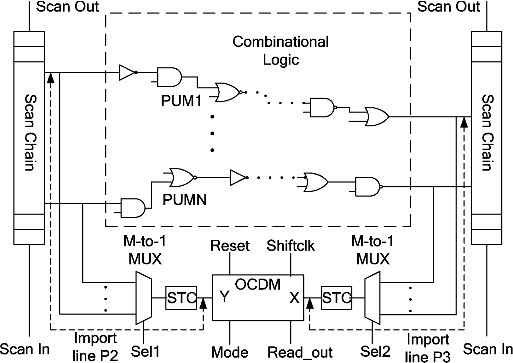
\includegraphics[width=0.65\textwidth]{OCDM-fig5}
   \caption{Path delay measurement architecture.}
    \label{fig:OCDM-fig5}
\end{figure}


\subsubsection{Signal Transition Conversion (STC)}
As mentioned in the previous section, the OCDM circuit works well only when the input and output of the PUM are rising transitions. However, there are other three additional cases possibly to activate the worst case delay of a circuit path, such as a path in which the input is a rising transition and the output is a falling transition. It is thus better to transfer the output signal into the signal with rising transition for facilitating path delay measurement regardless of the transition direction of the original signal.

The STC block shown in Figure \ref{fig:OCDM-fig5} is used to handle this problem. Therefore, rising transitions which are derived from the start and end points of PUM can be fed into the inputs and of the OCDM circuit, respectively. Figure \ref{fig:OCDM-fig6} shows the basic structure of the STC block, which is previously designed for signal stability violation detection in \cite{favalli1996sensing} \cite{agarwal2007circuit} \cite{yan2009unified}. The simplified timing waveform for the STC block is shown in Figure \ref{fig:OCDM-fig7}(a) and (b), respectively. When the pre-charge signal is low, denoted as the pre-charge period, both the nodes and are charged up to logic high values. Hence the OUT signal keeps a logic low value.

\begin{figure}[t]
\centering
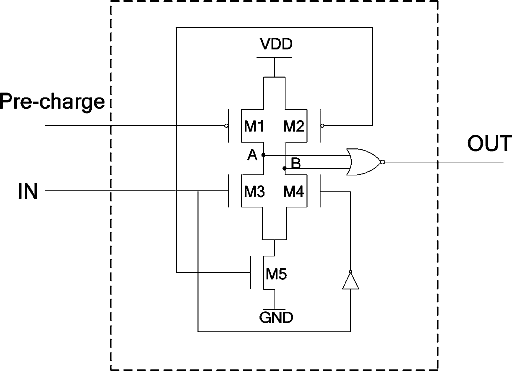
\includegraphics[width=0.65\textwidth]{OCDM-fig6}
    \caption{Signal Transition Conversion (STC).}
    \label{fig:OCDM-fig6}
\end{figure}

\begin{figure}[t]
\centering
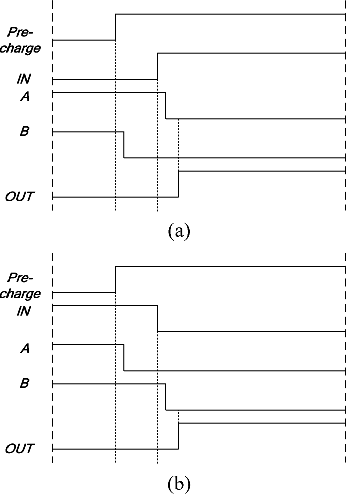
\includegraphics[width=0.6\textwidth]{OCDM-fig7}
    \caption{Simplified timing waveform for signal transition converter. (a) A rising transition at IN. (b) A failing transition at IN.}
    \label{fig:OCDM-fig7}
\end{figure}


Clearly, as shown in Figure \ref{fig:OCDM-fig7}(a), if a rising transition is generated at the IN signal when the pre-charge signal is high, both the node $A$ and node $B$ are discharged to logic low values after the arrival of the rising transition of IN. Therefore, a rising transition is generated at the OUT signal. Likewise, as shown in Figure \ref{fig:OCDM-fig7}(b), a rising transition would also be generated at the OUT signal after the arrival of a falling transition of the IN signal. Hence, by using the STC block, the input signal with arbitrary transition direction can be converted into a rising transition signal for facilitating path delay measurement.

\subsubsection{Delay Measurement}
The proposed on-chip delay measurement flow can be divided into eight steps as follows:
\begin{enumerate}[{1)}]
    \item Select the paths for delay measurement;
    \item For each PUM, the input and output transition signals of the PUM can be fed into the OCDM circuit for delay measurement by using the two M-to-1 multiplexes;
    \item The first vector of the test vector pair for the PUMis applied to initialize the internal logic of the circuit to a stable state; 
    \item All flip-flops of the OCDM circuit are initialized to logic ZERO values by asserting the reset signal; 
    \item The delay measurement mode is activated by asserting the mode signal; 
    \item The second vector of the test vector pair is applied to the circuit, and hence a transition signal can be launched at the input of the PUM, and propagated to the output of the PUM; consequently, the delay difference of the two transition signals is measured by the OCDM and recorded into the delay line; 
    \item After the completion of delaymeasurement, the OCDM circuit is configured into shift mode by de-asserting the mode signal. Therefore, the values stored in the delay line can be shifted out serially using clock signal shiftclk. Consequently, the path delay of the PUM can be calculated from the values read out.
\end{enumerate}

All paths can be selected for delay measurement by repeating the above steps 2–7.

After the values stored in the delay line have been read out, the delay of the PUM can then be obtained. Suppose the total number of delay stages in the OCDM circuit is $N$, the delay measurement resolution of the OCMD circuit is $M_{res}$, which is half of the delay range in the last delay stage $D_{las}$, and the values stored in the flip-flop from the first delay stage to the last delay stage of the OCDM circuit are $D_{N}$ to $D_{1}$, respectively. Then the path delay can be calculated as follows:


Delay of Measurement = $\sum_{i=1}^{i=N}D_{i} \times 2^{i-1}\times D_{las}$

The range of the path delay is then given as
$\sum_{i=1}^{i=N}D_{i} \times 2^{i-1} \times D_{las} - M_{res} <$ Path Delay $\sum_{i=1}^{i=N} \times D_{i} \times 2^{i-1} \times D_{las} + M_{res}$

The calculated path delay value of the PUM is then compared with the expected delay value for timing validation and silicon debug. The maximum delay measurement range of the OCDM circuit can also be obtained as follows.

Maximum measurement range = $\sum_{i=1}^{i=N} \times 2^{i-1} \times D_{las}$

\subsubsection{Delay Calibration for Import Lines}
In order to obtain the delay of the PUM with high precision, the delay of import lines $P_{2}$ and $P_{3}$ for feeding the start and end transitions of the PUM into the OCDM circuit, as shown in the Figure \ref{fig:OCDM-fig5}, should be taken into account. The reason is that it is difficult to mutually cancel the delays of the import lines $P_{2}$ and $P_{3}$ during physical design. Even though a careful custom layout can be conducted to balance the import lines $P_{2}$ and $P_{3}$ serving for one PUM, it can be hardly to satisfy this restriction for the import lines for all the PUMs. Moreover, the delays of import lines $P_{2}$ and $P_{3}$ would also be affected by the process variations and hence would bring a precision loss of the delay measurement. In order to address this problem, a 2-to-1 multiplexer is added for the flip-flop which is the end point of the PUM.


Figure \ref{fig:OCDM-fig8} redraws the architecture of the path delay measurement scheme shown in the Figure \ref{fig:OCDM-fig5}, which includes a 2-to-1 multiplexer with data inputs, respectively, connected to the data-input and data-output of the flip-flop at the end point of the PUM to calibrate the delay difference of import lines. 
\begin{figure}[t]
\centering
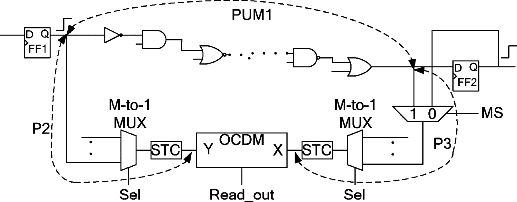
\includegraphics[width=0.8\textwidth]{OCDM-fig8}
    \caption{Delay calibration for improt lines}
    \label{fig:OCDM-fig8}
\end{figure}


When the MS signal is set to 1, the path delay measurement architecture is configured into the delay measurement mode. Hence the input and output of PUM1 are selected into the OCDM for delay measurement. The delay measurement result of PUM1 without considering the delay difference of import lines and can be represented as follows: 

Delay measurement result $= D_{1} + D_{3} - D_{2}$

where the $D_{1}$, $D_{2}$, and $D_{3}$ represent the delays of $PUM1$, $P_{2}$, and $P_{3}$, respectively. However, in order to obtain the delay of the PUM with high precision, the delay value of $D_{3} - D_{2}$ should be obtained firstly. The delay of $P_{3}$ is typically larger than that of $P_{2}$ for the insertion of a multiplexer. When the MS signal is set to 0, the import line’s delay difference calibration mode is configured.

For the first case, if the PUM is started at one flip-flop and ended at another flip-flop, then either rising or falling transition can be simultaneously generated at the outputs of the start and the end flip-flops by shifting the test vector with specific values into them. Hence the transitions generated at the outputs of the start and end flip-flops will pass through and into the OCDM circuit, respectively. Therefore, the delay difference of $P_{3}$ and $P_{2}$ can be obtained by the OCDM circuit under the import line’s delay difference calibration mode. For the second case, if the PUM is started and ended at the same flip-flop, then this scenario is even simpler. Either a rising or a falling transition generated at the output of the flip-flop can simultaneously pass through $P_{2}$ and $P_{3}$ into the OCDM circuit, respectively.

Consequently, by calibration the delay difference of the import lines for feeding the start and end transitions of the PUM into the OCDM circuit first, a high precision of path delay measurement can then be obtained.

\subsection{Experiment Result Analysis}
For validation, we implemented the proposed on-chip path delay measurement scheme using SMIC \SI{0.18}{\micro\metre} CMOS technology. The experimental results consist of the following five main parts: 1) simulated delay range for each delay stage of the OCDM circuit; 2) simulated results for measuring the delays of circuit paths using the proposed scheme; 3) validation of the effectiveness of the proposed scheme under process variations; 4) the hardware and timing overheads of the proposed scheme; and 5) comparisons with previous works.

\subsubsection{Experiment I}
In this experiment, six delay stages were designed in the OCDM circuit, making the maximum path delay measurement range of the OCDM achieves about 800 ps, while the delay range of the last stage is about 13 ps. The number of delay ranges in the OCDM circuit can be easily extended to achieve a much larger delay measurement range if required. 

The experimental result of the nominal delay range for each delay stage is reported in Table \ref{tab:delay-range}, which is obtained using HSPICE simulation. The delay range of each delay stage is approximately increased by a factor of two from the last to the first delay stage within a small margin of error. This ignorable error of delay range may be caused by the unbalanced load of each delay stage and the precision of HSPICE simulator. However, due to the fact that the delay measurement range of the OCDM circuit can be expanded exponentially by increasing the number of delay stages, thus we only need a small quantity of delay stages to achieve the required delay measurement range. Therefore, this error induced in the path delay measurement can be acceptable.

\begin{table}[h]
    \caption{Delay Range of Each Delay Stage} \label{tab:delay-range}
    \begin{tabular}{c|cccccc}
        \hline
         Delay Stage & 1 & 2 & 3 & 4 & 5 & 6 \\ \hline
         Delay Range (ps) & 409.7 & 205.1 & 102.84 & 51.59 & 25.91 & 13.23 \\ \hline
    \end{tabular}
\end{table}

\subsubsection{Experiment II}
In the second experiment, two different lengths of paths are chosen from ISCAS85 C880 benchmark to verify the effectiveness of the proposed on-chip path delay measurement scheme under the typical process corner.

The delay difference of the import lines can be obtained by the proposed on-chip delay measurement technique under the import line’s delay difference calibrationmode. In order to measure the delays of PUMs, path delay test vector pairs should be generated for the corresponding paths firstly. A transition is then launched at the input of the particular path which has been chosen for delay measurement using the generated test vector pair. The test vector generation method is beyond the scope of this paper.


Figure \ref{fig:OCDM-fig9} and Figure \ref{fig:OCDM-fig10} show the delay measurement results for the two paths obtained using HSPICE simulation, respectively. As shown in Figure \ref{fig:OCDM-fig9}(a), the delay of Path1 is 149.24 ps from HSPICE simulation. Figure \ref{fig:OCDM-fig9}(b) shows the simulated delay difference of the import lines, which are used to feed the start and end transitions of Path1 into the OCDM circuit. Every delay stage holds the initial logic ZERO value except for stage 2, stage 4, and stage 6 when the delay measurement is completed. Thus, the measured delay difference of the import lines is the sum of delay ranges in stage 2, stage 4, and stage 6, which can be calculated from Table \ref{tab:delay-range}, i.e., 270 ps in this case. Figure \ref{fig:OCDM-fig9}(c) shows the delay measurement result of Path1 for not considering the delay difference of import lines. Likewise, this delay measurement result can be obtained by summing the delay ranges of stage 1 and stage 6. Hence, the actual delay of Path1 can be obtained by subtracting the delay difference of import lines as obtained in Figure \ref{fig:OCDM-fig9}(b) from the path delay measurement result as obtained in Figure \ref{fig:OCDM-fig9}(c). As a result, the actual path delay of Path1 obtained by the proposed on-chip path delay measurement technique is 153 ps.

It can be observed from Figure \ref{fig:OCDM-fig10}(a) that the simulation delay of Path2 is 454.11 ps using HSPICE simulation. Under the import line’s delay difference calibration mode, the delay difference of the import lines which feed the start and end transition of Path2 into the OCDM circuit can be measured. The delay stage 3, stage 4, and stage 6 hold final stable logic ONE values after the import line’s delay difference calibration as shown in Figure \ref{fig:OCDM-fig10}(b). Hence the delay difference for the import lines is 167 ps. Likewise, the delay measurement result of Path 2, in which the delay difference of import lines is not taken into account, can be obtained by summing the delay ranges of stage 1, stage 2, and stage 6 as shown in Fig. 10(c). Hence, the actual path delay measurement result for Path2 can be obtained and is 460 ps. Through the aforementioned results, we have shown that the proposed on-chip path delay measurement scheme works well. It is worthy of note that the errors between the delay measurements and simulation values for the two paths are only 3.76 and 5.89 ps, respectively, and can be ignored.
\begin{figure}[t]
\centering
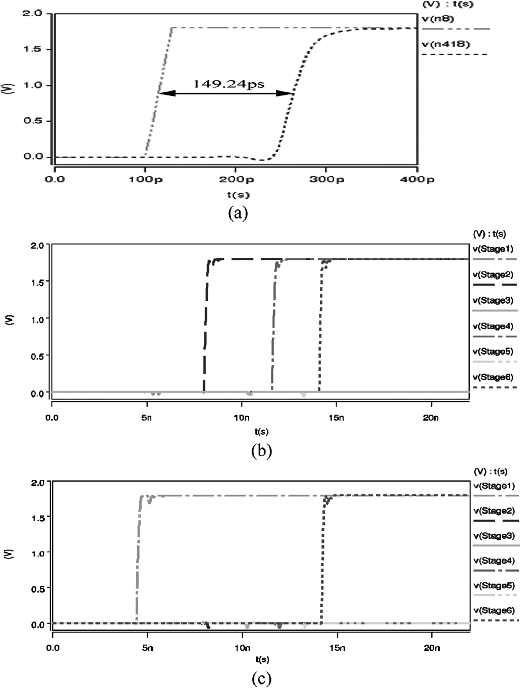
\includegraphics[width=0.75\textwidth]{OCDM-fig9}
    \caption{Simulated waveform for delay measurement of Path 1. (a) Delay from HSPICE simulation. (b) Delay difference of the import lines. (c) Delay measurement result of PUM.}
    \label{fig:OCDM-fig9}
\end{figure}

\begin{figure}[t]
\centering
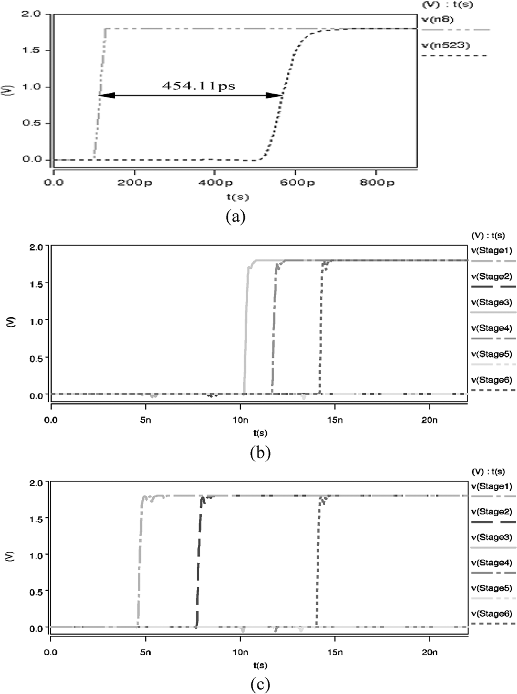
\includegraphics[width=0.75\textwidth]{OCDM-fig10}
    \caption{Simulated waveform for delay measurement of Path 2. (a) Delay from HSPICE simulation. (b) Delay difference of the import lines. (c) Delay measurement result of PUM.}
    \label{fig:OCDM-fig10}
\end{figure}

\subsubsection{Experiment III}
The circuit parameters are apparently prone to fluctuations caused by the significant process variations in sub-micro technologies. Hence the delays of circuit paths, import lines, and the delay ranges of the delay stages in OCDM circuit are thus unavoidable to suffer from undesirable variations. In this experiment, HSPICE Monte Carlo simulations are conducted to analyze the effectiveness of the proposed on-chip path delay measurement method in the presence of process variations. It is well known that the gate length variation poses a dominant impact on the gate delay \cite{nassif2000delay} \cite{agarwal2003statisticalc}. In our analysis, the inter-die and intra-die gate length variations are considered to have Gaussian distributions, $N(\mu_{L}, \delta_{1})$ and $N(\mu_{L}, \delta_{2})$, respectively \cite{wang2008path} \cite{tayade2008small}. The $\delta_{1}$ and $\delta_{2}$ represent the standard deviations of gate length for inter-die and intra-die variations respectively, while $\mu_{L}$ represents the transistor channel length obtained from the typical technology library.

Figure \ref{fig:OCDM-fig11}(a) and Figure \ref{fig:OCDM-fig11}(b) show the waveform of delay measurement results for Path1 and Path2, which are obtained from 50 Monte Carlo iterations considering both intra-die and inter-die variations. The variations considered in theMonte Carlo simulations are $3\delta_{1}=0.05\mu_{L}$ and $3\delta_{2}=0.05\mu_{L}$.

\begin{figure}[t]
\centering
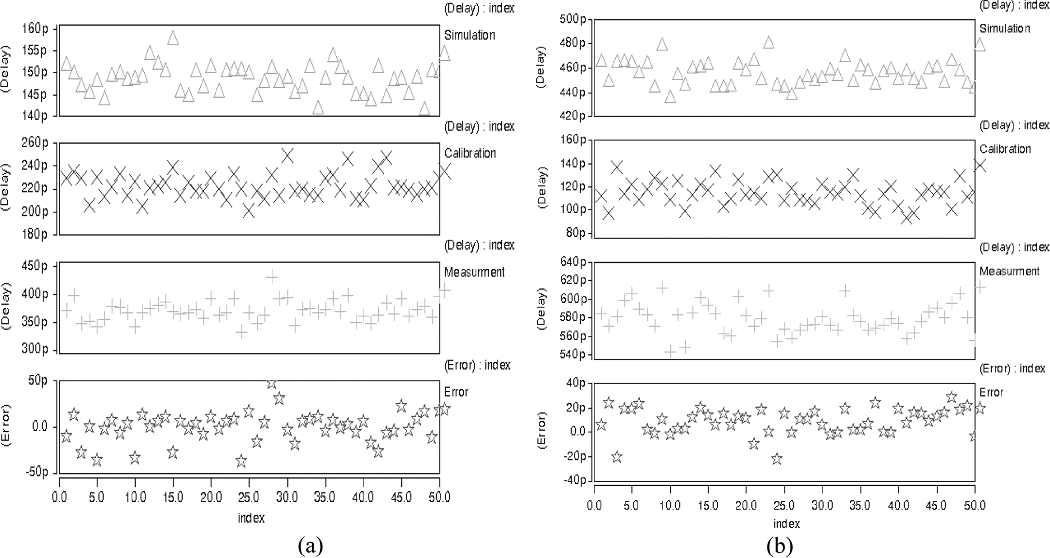
\includegraphics[width=0.95\textwidth]{OCDM-fig11}
    \caption{Simulated waveform for delay measurement obtained from 50 Monte Carlo iteration with $3\delta_{1}=0.05\mu_{L}$ and $3\delta_{2}=0.05\mu_{L}$ (a) for Path1 (b) for Path2.}
    \label{fig:OCDM-fig11}
\end{figure}


The panel indicated as Simulation in Figure \ref{fig:OCDM-fig11}(a) shows the simulation delay results of Path1 using HSPICE Monte Carlo method. Note that the delay of Path1 without considering process variations is 149.24 ps as shown in Figure \ref{fig:OCDM-fig9}. The delays of the import lines for feeding the start and end transitions of Path1 into the OCDM circuit would also be impacted by process variations. The panel indicated as Calibration in Figure \ref{fig:OCDM-fig11}(a) shows the delay measurement results of the delay difference between the corresponding import lines. The panel indicated as Measurement in Figure \ref{fig:OCDM-fig11}(a) shows the delay measurement results of Path1 without considering the delay difference of import lines $P_{2}$ and $P_{3}$. The panel indicated as Error in Figure \ref{fig:OCDM-fig11}(a) shows the errors between the delay measurement and simulation results for Path1 in the 50 Monte Carlo iterations, respectively. Likewise, the corresponding experimental results for Path2 are shown in Figure \ref{fig:OCDM-fig11}(b). Clearly, as shown in Figure \ref{fig:OCDM-fig11}, the error of path delay measurement conducted by the proposed scheme is very small, which demonstrates the effectiveness of the proposed path delay measurement scheme under process variations.


Figure \ref{fig:OCDM-fig12}(a) and Figure \ref{fig:OCDM-fig12}(b) show the Monte Carlo simulation results of delay measurement for Path1 and Path2 considering $3\delta_{1}=0.1\mu_{L}$ and $3\delta_{2}=0.1\mu_{L}$. It is clearly shown from Figure \ref{fig:OCDM_fig12} that although much larger delay variations are occurred as compared to the case in Figure \ref{fig:OCDM-fig11}, the error of path delaymeasurement results conducted by the proposed scheme is still very small, all within
the range of 50 ps.

\begin{figure}[t]
\centering
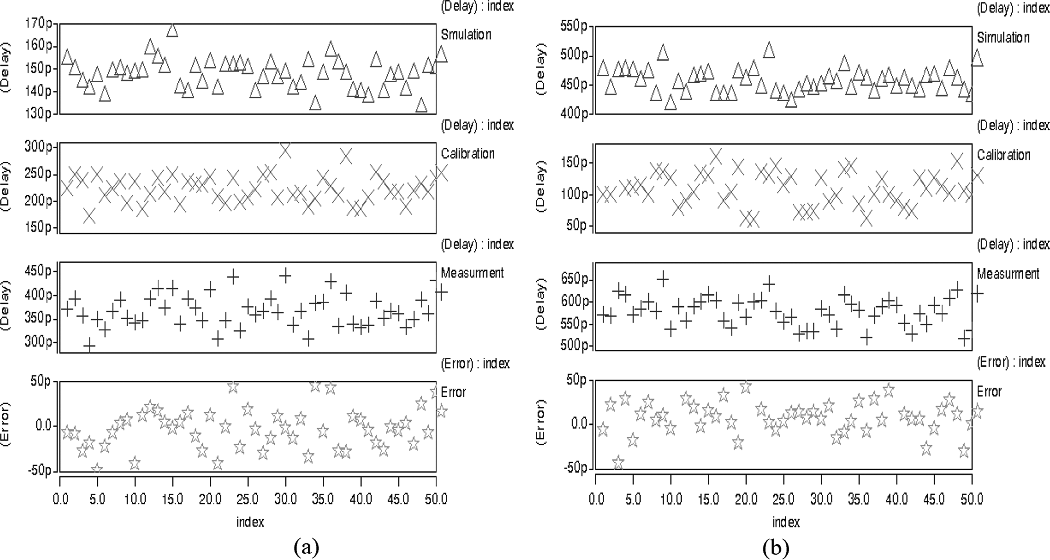
\includegraphics[width=0.95\textwidth]{OCDM-fig12}
    \caption{Simulated waveform for delay measurement obtained from 50 Monte Carlo iteration with $3\delta_{1}=0.1\mu_{L}$ and $3\delta_{2}=0.1\mu_{L}$, (a) for Path1 (b) for Path2.}
    \label{fig:OCDM-fig12}
\end{figure}


\subsubsection{Area and Timing Overhead}
In this experiment, the proposed path delay measurement architecture was incorporated into several IWLS 2005 full-scanbased benchmark circuits to evaluate its hardware and timing overheads. The area overheads reported in this paper are obtained by using a commercial synthesis tool targeting the SMIC \SI{0.18}{\micro\metre} CMOS technology. The benchmark circuits’ profiles and the area overhead of the proposed approach incorporated into the benchmark are presented in Table \ref{tab:area-overhead}. The circuit’s name of the benchmarks and the numbers of the flip-flops are given in column 1 and column 2, respectively. The column under “Circuit Area (\SI{}{\micro\metre^{2}})” reports the area of the benchmark circuits without implementing the proposed delay measurement architecture, while the sub-columns “Total”, “NoComb”, “Comb” represent the corresponding total, sequential, and combinational part’s area, respectively. Due to the different delaymeasurement requirements pursued by test experts, various path sets with totally different sizes and path delays may be selected for delay measurement. In this paper, we only focus on the delay measurement architecture rather than how to select the circuit paths targeting for delay measurement. Hence, we evaluate the area overheads of the proposed delay measurement architecture considering different numbers of path endpoints, even in the worst case where all the flip-flops are acted as the endpoints of paths for delay measurements. The columns “20\%M”, “60\%M”, and “100\%M” represent three cases in which 20\%, 60\%, and 100\% of the flip-flops are the endpoints of paths under measurements. For each of these flip-flops, a multiplexer is added to calibrate the delay difference of import lines. The sub-columns “Area ( \SI{}{\micro\metre^2} )” and “Area (\%)” under the three cases report the area overhead of the proposed delay measurement architecture and its percentage against that of the original benchmark circuit. 

\begin{table}[]
    \scriptsize
    \caption{Area Overhead of The Proposed Delay Measurement Architecture} \label{tab:area-overhead}
        \begin{tabular}{|c|c|ccc|cccccc|}
            \hline
            \multirow{3}{*}{Circuit} & \multirow{3}{*}{\# of FFs} & \multicolumn{3}{c|}{Circuit Area (\SI{}{\micro\metre^2})}                                                            & \multicolumn{6}{c|}{Area Overhead of the Proposed Scheme}                                                                                                                                                                         \\ \cline{3-11} 
                                     &                            & \multicolumn{1}{c|}{\multirow{2}{*}{Total}} & \multicolumn{1}{c|}{\multirow{2}{*}{NoComb.}} & \multirow{2}{*}{Comb.} & \multicolumn{2}{c|}{20\%M}                                                       & \multicolumn{2}{c|}{60\%M}                                                       & \multicolumn{2}{c|}{100\%M}                                 \\ \cline{6-11} 
                                                              &                            & \multicolumn{1}{c|}{}                       & \multicolumn{1}{c|}{}                         &                        & \multicolumn{1}{c|}{Area(\SI{}{\micro\metre^2})} & \multicolumn{1}{c|}{Area(\%)} & \multicolumn{1}{c|}{Area(\SI{}{\micro\metre^2})} & \multicolumn{1}{c|}{Area(\%)} & \multicolumn{1}{c|}{Area(\SI{}{\micro\metre^2})} & Area(\%) \\ \hline
                                                              des\_perf                & 8808                       & \multicolumn{1}{c|}{1196203}                & \multicolumn{1}{c|}{585978}                   & 610225                 & \multicolumn{1}{c|}{57037}                       & \multicolumn{1}{c|}{4.77\%}   & \multicolumn{1}{c|}{150794}                      & \multicolumn{1}{c|}{12.61\%}  & \multicolumn{1}{c|}{244550}                      & 20.44\%  \\ \hline
                                                              wb\_conmax               & 578                        & \multicolumn{1}{c|}{230776}                 & \multicolumn{1}{c|}{48243}                    & 182533                 & \multicolumn{1}{c|}{13235}                       & \multicolumn{1}{c|}{5,74\%}   & \multicolumn{1}{c|}{19388}                       & \multicolumn{1}{c|}{8.40\%}   & \multicolumn{1}{c|}{25540}                       & 11.07\%  \\ \hline
                                                              aes\_core                & 530                        & \multicolumn{1}{c|}{202325}                 & \multicolumn{1}{c|}{38699}                    & 163626                 & \multicolumn{1}{c|}{12980}                       & \multicolumn{1}{c|}{6.42\%}   & \multicolumn{1}{c|}{18621}                       & \multicolumn{1}{c|}{9.20\%}   & \multicolumn{1}{c|}{24263}                       & 11.99\%  \\ \hline
                                                              pci\_bridge32            & 3313                       & \multicolumn{1}{c|}{396500}                 & \multicolumn{1}{c|}{264226}                   & 132274                 & \multicolumn{1}{c|}{27792}                       & \multicolumn{1}{c|}{7.01\%}   & \multicolumn{1}{c|}{63057}                       & \multicolumn{1}{c|}{15.90\%}  & \multicolumn{1}{c|}{98322}                       & 24.80\%  \\ \hline
                                                              ac97\_ctrl               & 2229                       & \multicolumn{1}{c|}{237119}                 & \multicolumn{1}{c|}{174892}                   & 62227                  & \multicolumn{1}{c|}{22022}                       & \multicolumn{1}{c|}{9.29\%}   & \multicolumn{1}{c|}{45749}                       & \multicolumn{1}{c|}{19.29\%}  & \multicolumn{1}{c|}{69475}                       & 29.30\%  \\ \hline
                                                              mem\_ctrl                & 1126                       & \multicolumn{1}{c|}{158606}                 & \multicolumn{1}{c|}{92866}                    & 65740                  & \multicolumn{1}{c|}{16152}                       & \multicolumn{1}{c|}{10.18\%}  & \multicolumn{1}{c|}{28138}                       & \multicolumn{1}{c|}{17.74\%}  & \multicolumn{1}{c|}{40123}                       & 25.30\%  \\ \hline
                                                              usb\_funct               & 1741                       & \multicolumn{1}{c|}{242305}                 & \multicolumn{1}{c|}{127228}                   & 115077                 & \multicolumn{1}{c|}{1945}                        & \multicolumn{1}{c|}{8.02\%}   & \multicolumn{1}{c|}{37957}                       & \multicolumn{1}{c|}{15.66\%}  & \multicolumn{1}{c|}{56489}                       & 23.31\%  \\ \hline
                                                              systemcaes               & 670                        & \multicolumn{1}{c|}{139789}                 & \multicolumn{1}{c|}{55894}                    & 83895                  & \multicolumn{1}{c|}{13725}                       & \multicolumn{1}{c|}{9.82\%}   & \multicolumn{1}{c|}{20857}                       & \multicolumn{1}{c|}{14.92\%}  & \multicolumn{1}{c|}{27989}                       & 20.02\%  \\ \hline
        \end{tabular}
    \end{table}


As is clearly shown in the Table \ref{tab:area-overhead}, even in the worst case, the hardware overhead of the proposed delay measurement architecture can be acceptable. In practice, this scenario may be much more optimistic. For instance, Table \ref{tab:des-perf} reports the hardware overhead of the proposed architecture for des perf benchmark circuit, where all the critical paths that can be single-path sensitized are selected for delay measurement. As shown in Table \ref{tab:des-perf}, the clock period of the des perf circuit is synthesized to 2.6 ns by using a commercial synthesis tool, which guarantees a slack of 10\% the clock period for the longest path of the circuit under static timing analysis. The number of the selected critical internal paths is 1164, which is obtained by using a commercial timing analysis tool by specifying the path slack of which is less than 20\% of the clock period. For the selected critical internal paths, the number of paths that can be detected under the single path sensitization criterion is 779, which is obtained by using a commercial test generation tool and can then be sensitized for delay measurement. Clearly, multiple critical paths may be ended at the same endpoint. The number of endpoints for these paths suitable for delay measurement is 253. Therefore, only 253 endpoints should be inserted with the multiplexers to support the proposed delay measurement architecture. The area overhead of the whole proposed delay measurement architecture is \SI{116892}{\micro\metre^2}, and its percentage against that of the original benchmark circuit is only 1.41\%.

\begin{table}[]
    \scriptsize
    \caption{Experiment Results of DES\_Perf Circuit} \label{tab:des-perf}
    \begin{tabular}{|c|c|}
        \hline
        Benchmark                       & Des\_perf \\ \hline
        \# of FFs                       & 8808      \\ \hline
        Clock Period(ns)                & 2.6       \\ \hline
        \# of circuit critical paths    & 1164      \\ \hline
        \# of single path sensitization & 779       \\ \hline
        \# of critical endpoint         & 253       \\ \hline
        Area Overhead(\SI{}{\micro\metre^2})              & 16892     \\ \hline
        Area Overhead (\%)              & 1.41\%    \\ \hline
    \end{tabular}
\end{table}


Due to the application of the proposed delay measurement architecture, the delay of circuit paths may be impacted. Hence, the timing overhead of the delay measurement architecture to the critical path, which impacts the circuit performance, should be evaluated. Table \ref{tab:timing-overhead} evaluates the timing impact of the proposed delay measurement architecture to the delay of the longest circuit internal path in each benchmark circuit. The experimental circuit’s names and clock domains are listed in the column 1 and column 2, respectively. The columns under “Longest internal path delay (before)”and “Longest internal path delay (after)” represent the delays of the longest internal path before and after the incorporation of the delay measurement architecture for the considered clock domain. The column under “Delay increase” represents the delay increase of the longest path caused by incorporation of the proposed architecture. The column under “Timing overhead” represents the percentage of delay increase against the delay of the longest internal path before incorporation of the delay measurement architecture. As shown in Table \ref{tab:timing-overhead}, the timing impact of the proposed delay measurement architecture to the sample circuit is less than 0.7\% of the longest internal delay and can be negligible.

\begin{table}[]
    \scriptsize
    \caption{Timing Overhead}\label{tab:timing-overhead}
    \begin{tabular}{|c|c|c|c|c|c|}
        \hline
        Circuit       & clock domain     & \begin{tabular}[c]{@{}c@{}}Longest circuit internal \\ path delay (before) (ns)\end{tabular} & \begin{tabular}[c]{@{}c@{}}Longest circuit internal \\ path delay (after) (ns)\end{tabular} & \begin{tabular}[c]{@{}c@{}}Delay \\ increase (ps)\end{tabular} & \begin{tabular}[c]{@{}c@{}}Timing \\ Overhead(\%)\end{tabular} \\ \hline
            des\_perf     & clk              & 2.0280                                                                                       & 2.0377                                                                                      & 9.7                                                            & 0.48\%                                                         \\ \hline
            wb\_conmax    & clk\_i           & 1.9256                                                                                       & 1.9644                                                                                      & 11.8                                                           & 0.60\%                                                         \\ \hline
            aes\_core     & clk              & 2.7504                                                                                       & 2.7588                                                                                      & 8.4                                                            & 0.31\%                                                         \\ \hline
            pci\_bridge32 & pci\_clk\_i      & 1.7575                                                                                       & 1.7656                                                                                      & 8.1                                                            & 0.46\%                                                         \\ \hline
            ac97\_ctrl    & clk\_i           & 2.0684                                                                                       & 2.0790                                                                                      & 10.6                                                           & 0.51\%                                                         \\ \hline
            mem\_ctrl     & clk\_i           & 2.0788                                                                                       & 2.0931                                                                                      & 14.3                                                           & 0.69\%                                                         \\ \hline
            usb\_funct    & phy\_clk\_pad\_i & 1.8180                                                                                       & 1.8261                                                                                      & 8.1                                                            & 0.44\%                                                         \\ \hline
            systemcaes    & clk              & 3.0745                                                                                       & 3.0813                                                                                      & 6.8                                                            & 0.22\%                                                     \\ \hline 
    \end{tabular}
\end{table}

\subsubsection{Comparison A}
To compare with previous works, the delay measurement circuits using the proposed OCDM method and the method from \cite{datta2004chip} which employed a modified VDL with equal delay range value in each stage are implemented respectively. Table V compares the experimental results of the two methods. Note that the proposed OCDM circuit needs only 3.3\% of the delay stages to achieve even larger maximum delay measurement range compared to the delay measurement circuit using the method from \cite{datta2004chip}, while the delay measurement resolution of the proposed OCDM circuit is only 49\% of that for the delay measurement circuit using the method from \cite{datta2004chip}. As mentioned earlier, when the delay measurement is completed, the values stored in the flip-flops of the OCDM circuit should be shifted out serially using slow shift clock. If we assume the frequency of shift clock is 1GHz, then the time for scanning out themeasurement values is only 8ns for the proposed OCDM circuit, but is up to 245ns for the delay measurement circuit using the method from \cite{datta2004chip}.


\begin{table}[]
    \scriptsize
    \caption{Measurement Circuit Comparison}\label{tab:cmp}
    \begin{tabular}{|c|c|c|c|ccc|}
        \hline
        \multirow{2}{*}{Circuit} & \multirow{2}{*}{\begin{tabular}[c]{@{}c@{}}Stage \\ Numbers\end{tabular}} & \multirow{2}{*}{Resolution} & \multirow{2}{*}{\begin{tabular}[c]{@{}c@{}}Maximum \\ Measurement Range\end{tabular}} & \multicolumn{3}{c|}{Area (um2)}                                                    \\ \cline{5-7} 
                                     &                                                                           &                             &                                                                                       & \multicolumn{1}{c|}{Combinational} & \multicolumn{1}{c|}{No Combinational} & Total \\ \hline
                                     Proposed OCDM            & 8                                                                         & 6.62ps                      & 3295ps                                                                                & \multicolumn{1}{c|}{9547}          & \multicolumn{1}{c|}{612}              & 10159 \\ \hline
                                     {\cite{datta2004chip}}                 & 245                                                                       & 13.45ps                     & 3295ps                                                                                & \multicolumn{1}{c|}{26894}         & \multicolumn{1}{c|}{18744}            & 45638 \\ \hline
    \end{tabular}
\end{table}

The area overheads of the two delay measurement circuits are obtained using a commercial synthesis tool. It can be seen that the combinational, non-combinational, and the total area overheads of the proposed OCDM circuit are only 35.5\%, 3.3\%, and 22.3\% of that for the delay measurement circuit using the method from \cite{datta2004chip} respectively. It seems unfair to compare only the hardware overhead of the OCDM circuit of the proposed delay measurement architecture with the delay measurement circuit using themethod from \cite{datta2004chip} without considering the hardware overhead of the insertion of multiplexers at the endpoints of the PUMs. However, it should be noted that the OCDM circuit provides the same path delay measurement ability with that of the method from \cite{datta2004chip}, while the purpose of the insertion for 2-to-1 multiplexers to the end points of the PUMs is to calibrate the delay difference of import lines. Thereby, a higher precision of delay measurement results for the PUMs can be obtained by the proposed method as compared to the method from \cite{datta2004chip}.

\subsubsection{Comparison B}
By considering the delay difference of the import lines in the proposed scheme, and considering the returning loop delay in the Path-RO scheme \cite{wang2008path}, both the proposed scheme and the Path-RO scheme can provide a high precision for path delay measurement. However, as compared to the Path-RO technique, the proposed technique provides a more effective way to measure the delay of a path. This is mainly due to the following reasons.

1) A multiplexer is required to be inserted into the critical PUM in the Path-RO technique, which reduces the speed of high performance circuit. Clearly, in the proposed path delay measurement architecture, no extra cell has to be inserted in the PUM, while only a small overload from one input of the multiplexer is added in the PUM. Hence, the proposed technique has a weak impact to the delay of a critical path as compared to the Path-RO technique.

2) The Path-RO technique can only measure either the delays of paths that begin at a clocked flip-flop or the delays of paths that end at this clocked flip-flop. The reason is that the flip-flop which is the start point of the PUM has to be modified to a calibration launch flip-flop (CLFF), while the flip-flop which is the end point of the PUM has to be modified to a calibration capture flip-flop (CLFF) with a different circuit structure. However, the delay of each circuit path chosen for delay measurement can be obtained by the proposed on-chip path delay measurement technique.

3) In order to measure the delay of a path by using the Path-RO technique, one and two extra multiplexers are required to be added in the flip-flops which are stood at the input and output of the PUM, respectively. However, only one extra multiplexer is required to be added for the flip-flop which is the endpoint of the PUM in the proposed path delay measurement technique. Hence, the proposed method suffers from a significant lower hardware overhead as compared to the Path-RO technique.

4) By using the Path-RO technique, only the delay of a path on which the number of inverting logics is odd can be measured due to the use of the oscillation technique. Otherwise, one inverter is required to be added to the PUM, which will further increase the design complexity to the path delay measurement architecture. Moreover, the delay of the returning loop might not be calibrated to a clock period because the first requirement of the calibration process is to assure that the PUM is configured to be able to oscillate. Hence, the precision of the path delay measurement would be influenced. Clearly, no such extra restrictions are posed into the proposed on-chip path delay measurement technique when measuring the delay of a chosen circuit path.

\subsection{Discussion}
In this paper, we have presented a novel on-chip path delay measurement technique for timing characterization and silicon debug. In the proposed OCDM circuit, the delay range of each delay stage is set to increase by a factor of two gradually from the last to the first delay stage. In addition, by conducting delay compensation, both improved delay measurement resolution and measurement precision can be provided when compared to the previous VDL based delay measurement schemes. The delay difference of the import lines for feeding the start and end transitions of the PUM into the OCDM circuit is also considered in the proposed technique, which can further provide a high precision for path delay measurement. Experimental results show that the proposed on-chip path delay measurement scheme works well. A small quantity of delay stages in OCDM circuit can obtain a large delay measurement range, and hence can provide a significant reduction in delay measurement time. Moreover, the area overhead of the proposed method is also significantly reduced as compared to previous works.

\section{Lifetime Fault-Tolerant Circuit Design}
In the past decades, the device and reliability communities have devoted much efforts to lifetime projection \cite{Sony}\cite{Atmel}, but less to design for lifetime reliability. This situation would be changed because the lifetime reliability is seriously challenged by the aggressive technology scaling \cite{degradation_05}\cite{ITRS_PIDS07}. One of the major impending (above 22nm) challenges comes from MOS transistor wearout \cite{ITRS_PIDS07}; NBTI (Negative Bias Temperature Instability)  and TDDB (Time Dependent Dielectric Breakdown) draw the most attentions over a wide variety of transistor aging mechanisms \cite{ITRS_PIDS07}. Both aging mechanisms can gradually degrade the performance of transistors over time \cite{failure_prediction_07}\cite{Self-calibrating_07} due to elevated threshold voltage \cite{NBTI_Impact05}\cite{Impact-of-NBTI_07} or degraded integrity of gate oxide \cite{OB_Invert_03}\cite{Impact_BD_04}\cite{Gate-oxide-breakdown-07}.

To guarantee the chips' lifetime reliability, a common practice is reserving conservative timing margin---just like that for process variations \cite{ParameterVariations_DAC03}. However, the effectiveness of such approaches is diminishing, given that up to 10-20\% guardband has to be reserved to safely accommodate the aging-induced performance degradation---which can even offset the performance benefit from one-generation of technology advancement.

Many researches have been conducted at different levels: device level \cite{DynamicNBTI_03}\cite{Modeling-and-minimization_06}, circuit level \cite{Compact-Modeling_07}\cite{Impact-of-NBTI_07}, and (micro)architecture level \cite{RAMP_04}\cite{Penelope_07}\cite{Framework_DSN07}. Particularly, Blome et al. proposed an online wearout detection approach through sensing the aging-induced delay \cite{Self-calibrating_07}. Agarwal et al., based on the same observation, proposed a sensor design dedicated for aging failure prediction \cite{failure_prediction_07}. Yan et al. presented a more versatile and cost efficient sensor design \cite{SVFD_09} which can also be used for aging detection.

Although the prior sensor designs prepare a ground for aging-aware designs, few researches are conducted so far to study how to effectively use them; this work aims to serve this purpose. The lifetime of a chip is governed by the "weakest-link principle"---usually only a minority of transistors suffer large aging degradation reflected in excessive path delay. The aging sensors can capture this change; however, previous solutions such as turning voltage and/or frequency \cite{RAMP_04}, reducing individual core utilization \cite{Facelift_08}, and duplicating hardware resources \cite{Duplication_05}\cite{WearoutRecovery_08} do not use such fine-grained detection capability sufficiently. Although those architecture- and application-level approaches are somewhat effective to remedy the aged chips, these coarse-grained solutions trading either performance or hardware resources for lifetime may be far from efficient due to the blindness to the minority of fine-grained "weakest links" which can be identified by the aging sensors.


Above analysis motivates us to propose a new approach to exploiting fine-grained aging adaptability. Unlike those coarse-grained approaches, the fine-grained approach can cope with the "weakest-links" more locally and efficiently, thereby making it possible to improve lifetime reliability while without compromising with the architectural performance and coarse-grained hardware resources. In particular, we make three contributions:
\begin{enumerate}
\item We propose ReviveNet, a hardware-implemented aging-aware and self-adaptive architecture, to improve lifetime reliability. Aging-awareness is realized by deploying dedicated aging sensors, and "self-adaptive" is achieved by employing a group of synergistic adaptation agents.

\item To support ReviveNet, we present a localized timing adaptation mechanism, with which the aged critical paths can be locally coped with. The fine-grained adaptability results from timing imbalance between consecutive timing paths. The lifetime can be extended significantly through exploiting such "path-grained" adaptability.

\item We propose an evaluation model to quantitatively study the ReviveNet-enhanced reliability.
\end{enumerate}

The effectiveness of ReviveNet has been evaluated through incorporating it into an industrial pipelined floating-point co-processor. Experimental results show that ReviveNet can improve the MTTF by 48.7\% without compromising with architectural performance, only at about 9.5\% area and small power overhead.


\subsection{Aging Symptoms and Aging Sensors}
The aging-induced delay is a suitable symptom candidate \cite{Self-calibrating_07} \cite{failure_prediction_07} \cite{failure_prediction2_08}. For example, Blome et al. took the TDDB induced delay as the symptom for wearout detection \cite{Self-calibrating_07}. Agarwal. et al, took the NBTI induced delay as the symptom for aging failure prediction \cite{failure_prediction_07}\cite{failure_prediction2_08}. We also take aging delay as the symptom in this work.

Aging-awareness can be realized by employing some dedicated aging sensors. The fundamental working principle of sensors is on-line delay fault detection. The only difference between the aging sensing and traditional delay fault detection is that the former takes place in a safe timing interval called "Guard band" \cite{failure_prediction_07}, while the latter takes place in the interval after the effective clock edge called "Detection slack" \cite{SVFD_09}. As Figure \ref{agingdelay} shows, initially, in fresh state, no signal transitions occur in guard band, but after suffering form aging, some transitions could be delayed into guard band. Since the signal should have been stabilized before entering the guard band, we call the event of such a ``faulty" transition in guard band as a Stability Violation \cite{SVFD_09}. It is worthy to note that the detected aging delay, unlike conventional delay faults, won't cause any timing fault (a.k.a. Timing violation).

\begin{figure}[t]
\centering
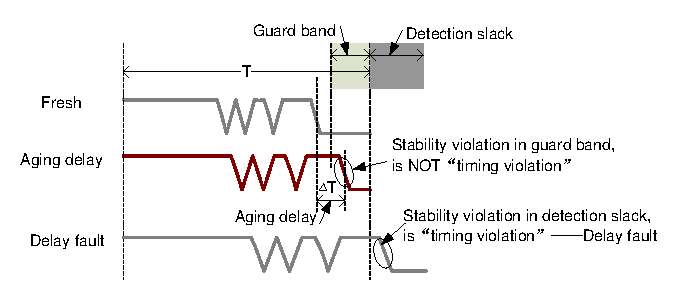
\includegraphics[width=0.5\textwidth]{fig2-12.eps}%{agingdelay.eps}
   \caption{The timing of Aging delay and delay fault}\label{agingdelay}
\end{figure}

\begin{figure}[t]
\centering
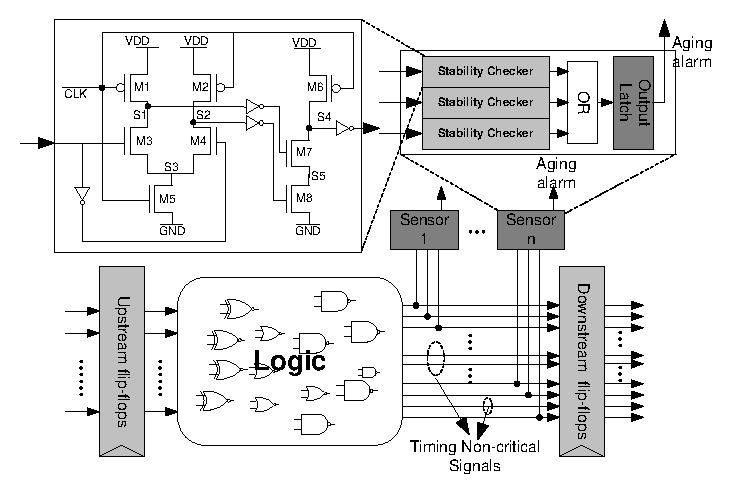
\includegraphics[width=0.5\textwidth]{fig2-13.eps}%{sensorsetup.eps}
\vspace{-0.5cm}
   \caption{Sensor setup}\label{setupsonsor}
\end{figure}

The detection for aging delay is actually to detect the stability violations in guard band. We can use stability checker---the key component in aging sensor---to fulfill this purpose. The basic stability checker can be derived from a sensing circuit for on-line delay fault detection, in which the signal integrity is verified by a pair of consistent charge/discharge nodes, the delay transitions will trigger one of the charged nodes to be discharged and thereby causes state inconsistence between them. More specifically, as shown in Fig \ref{setupsonsor}, during precharge period, both nodes $S1$ and $S2$ in the stability checker are charged up to HIGH. The circuit starts evaluation when entering the guard band; one of the two nodes is pulled down, while the other one floats at HIGH because the gate signal of M3 is always complemented with that of M4. Hence, the node $S1$ and $S2$ are always exclusive during fault-free time, which will make the node $S4$ stick to HIGH because the high-impedance path between S4 and GND always exists. When aging delay happens, the stability violation will trigger the discharge of the node that has charged up to HIGH. Eventually both nodes are discharged, and thereby the node S4 is pull down to LOW---which flags aging delay being detected. Please refer to \cite{SVFD_09} for more details.

One sensor consists of multiple stability checkers, one wide dynamic OR gate, and one output latch \cite{SVFD_09}. To reduced overhead, multiple stability checkers share one output latch through a wide dynamic OR gate, as shown in Figure \ref{setupsonsor}.

The aging sensors are deployed to monitor critical paths. As an example, Figure \ref{setupsonsor} shows a setup for a stage of logic, where each sensor handles three signals. If some aged transistors in the logic or upstream flip-flops result in stability violations in the guard band---aging delay, the corresponding sensors can tell that an aging failure is impending.

With the "awareness" of aging, the next essential problem is how to accommodate the impending aging failures indicated by these alarms. The ReviveNet aims to address this problem.

\subsection{Lifetime Fault-tolerant Architecture}

Figure \ref{syntop} illustrates the ReviveNet architecture. Each stage is monitored by a set of periodically-invoked aging sensors. The adaptation to each stage is implemented with a set of adaptation agents which are fed by not only the local stage's aging sensors but also the next stage's agents, thereby enabling bidirectional adaptation\,---\,\emph{backward timing adaptation} (BTA) and \emph{forward timing adaptation} (FTA).  BTA is using the $(K+1)$st stage's timing slack to accommodate the aging emergencies in the $K$th stage, while FTA is using the $(K-1)$st stage's slack to accommodate the emergencies in the $K$th stage.  With the bidirectional adaptation mechanism, ReviveNet offers more adaptation freedom and performs more effectively.


\begin{figure}[t]
\centering
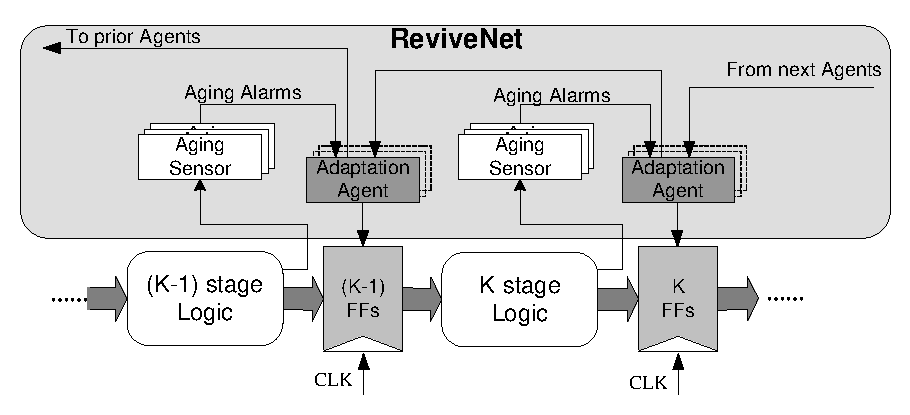
\includegraphics[width=0.7\textwidth]{fig2-14.eps}%{revivenet.eps}
   \caption{ReviveNet architecture}\label{syntop}
\end{figure}

\begin{figure}[h]
 \centering
  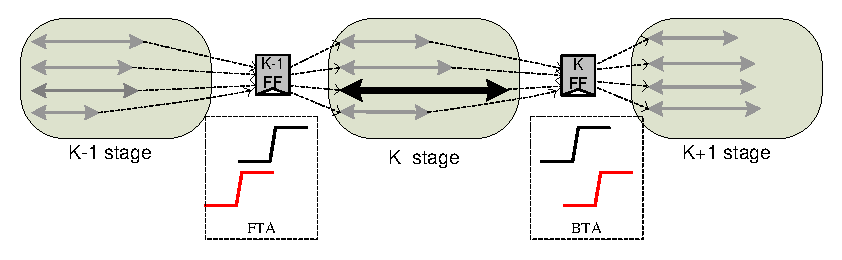
\includegraphics[width=0.7\textwidth]{fig2-15.eps}%{ba_fa.eps}
  \caption{Example of adaptation}\label{ba_fa}
\end{figure}

Let's explain the basic idea of ReviveNet with a simple example. Figure \ref{ba_fa} shows a part of a pipeline, where each arrow denotes a timing path and the length of it represents corresponding delay; in particular, the critical path in the middle stage is denoted by a bold arrow. After experiencing some aging, suppose that the delay of the critical path is going to exceed the clock period---an impending aging failure, an aging sensor monitoring this path detects the impending failure \cite{failure_prediction_07}\cite{SVFD_09} and flags an aging alarm; then, three local adaptation options can be enabled to tolerate this aging delay: 1) backward skew the clock of $K$th flip-flop---BTA, 2) forward skew the clock of $(K-1)$st flip-flop---FTA, or 3) both FTA and BTA. The specific adaptations are governed by a finite state machine, referred to agent.

The above conceptual example can just convey a very basic idea of ReviveNet; we can gain more insights into the ReviveNet's operations and underling design tradeoffs by answering the following questions:

{\bf 1) Why are BTA and FTA feasible?}

Clearly, BTA or FTA can help tolerate the aging delay of the target critical path only if there is timing imbalance between the corresponding paths, i.e. all upstream paths of $(K-1)$st flip-flop, or all downstream paths of $K$th flip-flop are non-critical. We call such imbalance as path-grained (or, localized) adaptability. We will use a case study (Section XXX investigation) to show that the potential of such localized adaptability, which ReviveNet aims to exploit, is quite attractive.

{\bf 2) Where the sensors and agents should be deployed?}

This problem is trivial if both the critical paths and aging impacts can be well-predicted: every critical path that is prone to suffer aging impacts should be monitored by a sensor. Unfortunately, though the critical paths can be somewhat distinguished from non-critical paths with some sophisticated SSTA (statistical static timing analysis) approaches, many researches have been evident that the aging degree of individual transistor highly depends on the physical geometries, defect density and the stress states during working mode. In other words, the aging degree of individual transistor is highly unpredictable; hence it seems hopeless to identify the aging-prone critical paths. We take an engineering way to tackle this problem: conservatively put all critical paths under monitor. Thought it is not an theoretically optimum option, the experimental results show that such engineering way is still cost-efficient (Section XXX Case Study).

Deploying agents is based on the sensors deployment and specific circuit topology. The detail can be found in (Section XXX Deploy Agent Sensor).

{\bf 3) What's the adaptation logic of agents?}

Usually, one sensor is able to monitor multiple critical paths to reduce the implementation overhead. The side-effect is decreased "resolution"---when a sensor flags an aging alarm, the agent actually cannot immediately recognize that which path (or paths) causes this alarm; hence the agent needs to follow a policy to efficiently identify the root of the alarm. Given that the aging is a progressive process and thus does not need to be in realtime accommodated, we propose a round-robin trial adaptation mechanism---the agent travels across a set of prioritized adaptation states to track back the source of the alarm and then tries the best to accommodate it (Section XXX RRTA).


{\bf 4) How to implement the intentional clock skew?}

The intentional skew is used to enable BTA and FTA.  One way to obtain the intentional skew is by inserting delay buffers \cite{Recycle_07}. However, the drawback of such delay-buffer based design is poor controllability. For example, suppose that during the early years of service life almost no adaptation is required, but these buffers still suffer from aging, contribute to leakage power, and so on. We propose a new implementing scheme to obtain the skewed clocks in a highly controllable way, while minimizing the side effects to the adaptation-free period (Section XXX Clcok Gen, XXX Clock Gate).


{\bf 5) What if the infrastructure of ReviveNet, sensors and agents, fail to work due to aging?}

ReviveNet is relatively aging resistant because it does not need to be always-on; most of lifetime it is power-off. Thus, the transistors' aging rate in sensors and agents, statistically, is much slower than that in host logics. We shall give more detailed discussion in Next Section.


{\bf 6) How much extended lifetime can be achieved?}

This question is hard to answer due to lack of accurate models that capture the relationship between a variety of aging mechanisms and aging delay. To quantitatively study the MTTF (Mean-Time-To-Failure) improvement, we propose a ReviveNet-enhanced  reliability model in which the relationship is condensed to a hypothetical function $\delta$ (Section XXX Model). Then, we instantiate the function based on the well-studied NBTI mechanism (Section XXX Case Study) to show the effect of ReviveNet, though the reliability model can also be applied to other aging mechanisms that need more intensive studies in the future. Experimental results show that up to 48.7\% MTTF improvement can be achieved.


Figure \ref{curve} qualitatively shows the ReviveNet-enhanced lifetime. When ReviveNet is too exhausted to make any effective adaptation---if any of the agents fails to accommodate an impending aging failure, the chip is judged reaching the end of lifetime. ReviveNet can also readily indicate the "incurable" failure; then, one can proactively take actions, such as replacing the aged chips, degrading the architectural performance, to minimize the impacts of failure.


\begin{figure}[t]
\centering
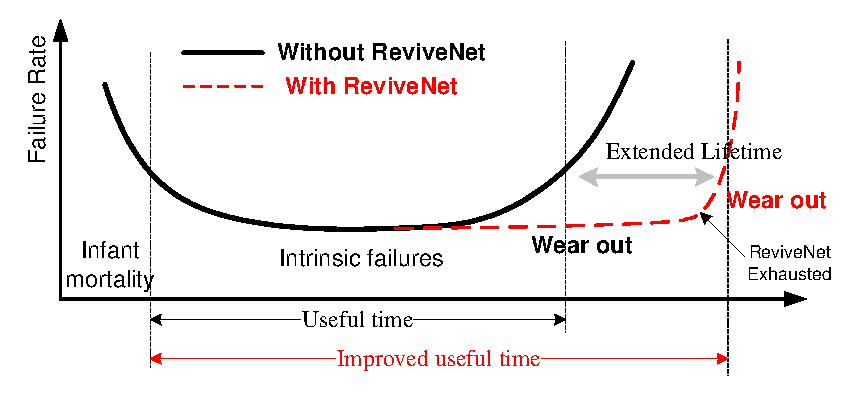
\includegraphics[width=0.75\textwidth]{fig2-16.eps}%{curve.eps}
   \caption{Anticipated effect of ReviveNet}\label{curve}
\end{figure}

\subsection{Self-Adaptive Fault-Tolerant Pipeline}
\subsubsection{Timing Imbalance}
We describe the timing imbalance that can be exploited to tolerate the aging delay through characterizing pipeline flip-flops. A pipeline flip-flop can be categorized according to the slack values of related upstream and downstream paths. Specifically, suppose a flip-flop $FF$ serves as the end point of $m$ paths with slack values $e_1$, $e_2$, $\ldots$, $e_m$, and the start point of $n$ paths with slack values $s_1$, $s_2$, $\ldots$, $s_n$. Given a threshold, $TH$, which distinguishes the (potential) critical paths ($slack \leq TH$) from others ($slack > TH$), the flip-flop must fall into one of the four classes:

$\bullet$ Generous Flip-flop (GFF):  $\forall e_i\in$ \{$e_1$, $e_2$, $\ldots$,
$e_m$\}, s.t. $e_i>TH$, and $\forall s_j\in$ \{$s_1$, $s_2$, $\ldots$, $s_n$\}, s.t. $s_j>TH$ (say, ``Generous" with timing margin).

$\bullet$ Backward Adaptable Flip-flop (BAFF):  $\exists e_i\in$ \{$e_1$, $e_2$, $\ldots$,
$e_m$\}, s.t. $e_i\leq TH$, but $\forall s_j\in$ \{$s_1$, $s_2$, $\ldots$, $s_n$\}, s.t. $s_j>TH$.

$\bullet$ Forward Adaptable Flip-flop (FAFF):  $\forall e_i \in$ \{$e_1$, $e_2$, $\ldots$,
$e_m$\}, s.t. $e_i>TH$, but $\exists s_j\in$ \{$s_1$, $s_2$, $\ldots$, $s_n$\}, s.t. $s_j\leq TH$.

%FAFFs and BAFFs can also serve as margin providers, although in a ``unidirectional" manner.

$\bullet$ Unadaptable Flip-flop (UAFF):  $\exists e_i\in$ \{$e_1$, $e_2$, $\ldots$,
$e_m$\}, s.t. $e_i\leq TH$, and $\exists s_j\in$ \{$s_1$, $s_2$, $\ldots$, $s_n$\}, s.t. $s_j\leq TH$.


In the following cases can yield critical paths:
\begin{enumerate}
\item  start with a FAFF and end with a BAFF, or
\item  start with a FAFF and end with a UAFF, or
\item  start with a UAFF and end with a BAFF, or
\item  start with a UAFF and end with a UAFF.
\end{enumerate}

A critical path in case 2) and 3) can gain extra $TH/2$ slack (note that we let the slack-providing paths still hold at least $TH/2$ slack); that in case 1) can gain extra $TH/2+TH/2$ slack; while that in case 4) cannot gain any extra slack.


Threshold $TH$ is a key factor affecting the design tradeoffs. On one hand, the larger $TH$, the higher percentage of UAFFs, thus more critical paths will be rendered unadaptable; on the other, the larger $TH$ can facilitate more aggressive time stealing on adaptable paths. In (Section XXX Case Study), we will show that neither over-large nor over-small $TH$ can lead to an optimum design tradeoff.

\subsubsection{Self-Adaptive Design Example}
As a case study, the following investigates the intrinsic timing imbalance in a industry design.

\begin{figure}[t]
\centering
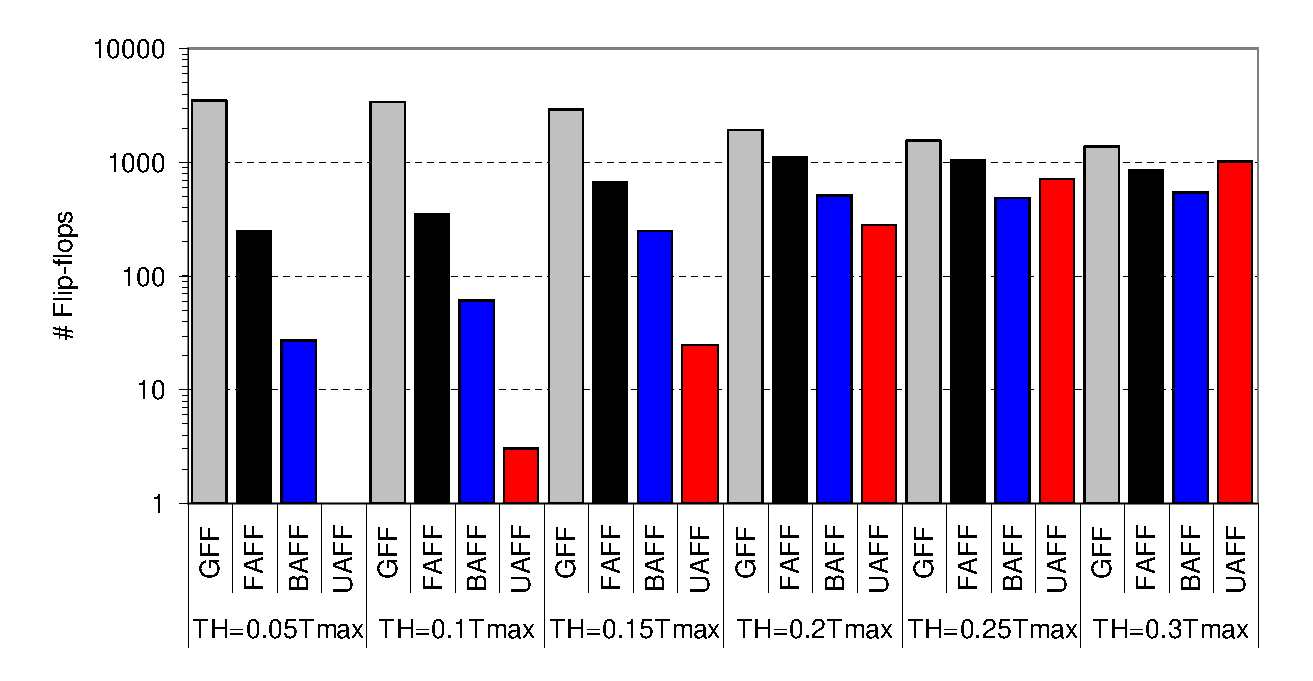
\includegraphics[width=0.75\textwidth]{fig2-17.eps}
    \caption{Distribution of flip-flops at different $TH$}\label{ff_type}
\end{figure}

We took a pipelined FPU adopted by OpenSPARC T1 \cite{OpenSPARC_06} processor as our target circuit. This FPU is synthesized using Synopsys Design Compiler with UMC 0.18um technology, and its' path timing is analyzed with PrimeTime. We set the performance as the synthesizing priority to smooth the distribution of path delay as much as possible. The timing analysis results are shown in Figure \ref{ff_type}.

Figure \ref{ff_type} shows the breakdowns of flip-flops with different type of adaptability, under six $TH$ configurations: 0.05 ($T_{max}$), 0.1, 0.15, 0.2, 0.25, and 0.3, where $T_{max}$ represents the most critical path delay. When $TH$=0.05, all of the critical paths are adaptable due to no  UAFF appears. With $TH$ increasing, some GFFs fall into the groups of BAFFs or FAFFs, even UAFFs, but GFFs, BAFFs and FAFFs always take considerable percentage---that is the ``potential" (localized adaptability) which ReviveNet can exploit.

\subsection{Self-adaptive Agent} \label{agentdesign}
The agents are responsible for controlling the localized adaptations. Before delving into the implementation details, let's first suppose that such localized adaptations can be realized by selecting a clock from multiple available clocks skewed from each other, as Figure \ref{affs} shows. The adaptability of each flip-flop has been identified beforehand with a static timing analysis tool. The GFFs' and UAFFs' clocks are kept intact, and each FAFF's, BAFF's clock is individually controllable. Dealing with UAFFs in this way is because no favorable time margins can be exploited without hurting the timing of other critical paths, so we would rather keep them intact than take tentative adaptations which cannot guarantee any reliability benefits. A FAFF is clocked by either original clock (CLK) or forward skewed clock (FCLK) to enable FTA; a BAFF is clocked by either CLK or backward skewed clock (BCLK) to enable BTA.

\begin{figure}[t]
\centering
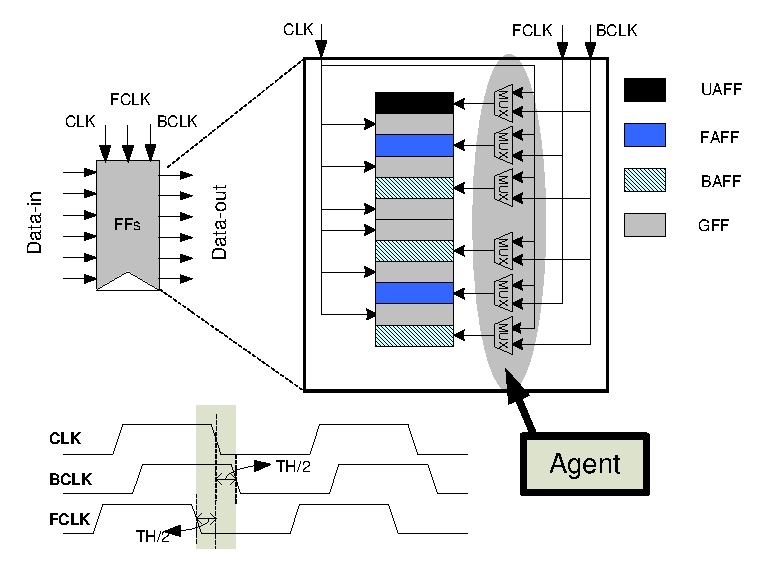
\includegraphics[width=0.75\textwidth]{fig2-18.eps}
   \caption{Example of adaptive clock assignment (agent is responsible for
   generating the clock-steering signals)}\label{affs}
\end{figure}

In Figure \ref{affs}, suppose that a sensor is deployed to monitor all of UAFFs and BAFFs, when the sensor flags an aging alarm, how does the corresponding agent perform the clock steering? One way is to enable all of the BAFFs (the FAFFs are enabled by the next stage's agent and discussed later); however, such "brutal" way may significantly sacrifice the timing margins of the innocent paths, thus not complying with the principle of "localized adaptation". The following presents a trial-based approach to address this problem.

\subsubsection{Round-Robin Trial Adaptation (RRTA)}\label{section_rrta}

When a sensor raises an aging alarm, it could be traced back to single or multiple critical paths. Fortunately, given that circuit aging usually is a gradual process, the response of an intended adaptation does not need to be in realtime. This allowable adaptation latency can justify the proposed RRTA approach below.

RRTA performs in an "identify-then-adapt" manner. Each trial represents an adaptation state---the value of clock-steering signals of related flip-flops. Figure \ref{rradp} presents the procedure of RRTA.

\begin{figure}[h]
\centering
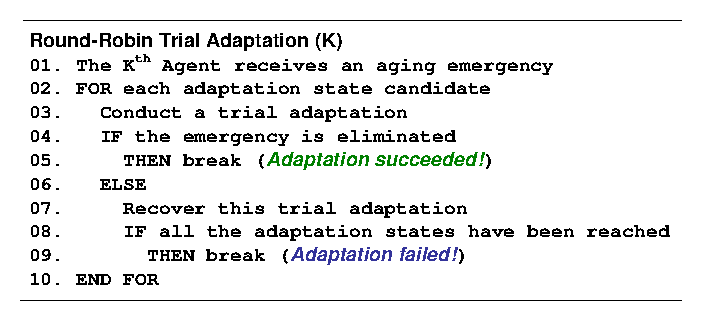
\includegraphics[width=0.7\textwidth]{fig2-19.eps}%{rrta.eps}
   \caption{Round-Robin Trial Adaptation}\label{rradp}
\end{figure}

The following clarifies how to define the set of adaptation states (related to line 2 in Figure \ref{rradp}). Generally, each agent is fed by an aging alarm and a request from another agent (as shown in Figure \ref{syntop}). For agent $A_K$ and a set of flip-flops $FF$, the aging alarms only trigger the backward adaptations to BAFFs, and the requests triggers the forward adaptations to FAFFs. The adaptation states are described with the following example.

\exmp\label{rrtaexample}  For the $K$th stage with downstream flip-flops $FF_k$=\{$f_1^k$, \ldots, $b_1^k$, $b_2^k$, $b_3^k$, $u_1^k$\} and upstream flip-flops $FF_{k-1}$=\{$f_1^{k-1}$, $f_2^{k-1}$, $f_3^{k-1}$, $f_4^{k-1}$, $b_1^{k-1}$, \ldots, $u_1^{k-1}$, \ldots\}, where $f$, $b$, and $u$ denote FAFF, BAFF, and UAFF, respectively. Agent $A_K$ and  $A_{K-1}$ handles $FF_k$ and $FF_{k-1}$, respectively. Clearly, only \{$b_1^k$, $b_2^k$, $b_3^k$\} and \{$f_1^{k-1}$, $f_2^{k-1}$, $f_3^{k-1}$, $f_4^{k-1}$\} can contribute to the $K$th stage's adaptations. Furthermore, suppose that only $f_1^{k-1}$, $f_2^{k-1}$, $f_3^{k-1}$, $f_4^{k-1}$ are related inputs to $b_1^k$, $b_2^k$, $b_3^k$. The correspondence of related FAFFs and BAFFs is easy to identify with logic core generation algorithms which has been well-studied and widely used on ATPG (Automatic Test Patten Generation) \cite{POIROT_00}.

The candidates of backward adaptation states (BAS) are denoted by $BAS$=$BAS_0$ $\cup$ $BAS_1$ $\cup$ $BAS_2$ $\cup$ $BAS_3$ where each term is a set of states corresponding to $b_1^k$, $b_2^k$, and $b_3^k$, as follows: 
{\small\begin{align}
BAS_0=\;&\{000\};            \nonumber \\
BAS_1=\;&\{001, 010, 100\};    \nonumber\\
BAS_2=\;&\{011, 101, 110\};  \nonumber \\
BAS_3=\;&\{111\}          . \nonumber
\end{align}}

$BAS_0$ is an initial state representing no adaption conducted. $BAS_1$, $BAS_2$, and $BAS_3$ represent 1-bit, 2-bit, and 3-bit backward adaptations conducting on $b_1^k$, $b_2^k$, and $b_3^k$, respectively. The agent, for example, conducts a "001" adaptation, means that BCLK for $b_3^k$ is enabled, while keeping the $b_1^k$, $b_2^k$ intact. Clearly, the perturbation level to the circuit is elevated from $BAS_1$ to $BAS_3$ because more bits adapted implies more perturbations introduced.

On the other hand, if $A_K$ receives an aging alarm, there should be another option: forward adapting the FAFFs in $FF_{k-1}$. To do so, $A_K$ needs to cooperate with $A_{K-1}$. The corresponding candidates of forward adaptation states (FAS), similarly to $BAS$, can be defined as $FAS$=$FAS_0$ $\cup$ $FAS_1$ $\cup$ $FAS_2$ $\cup$ $FAS_3$ $\cup$ $FAS_4$, where

{\small\begin{align}
FAS_0=\;&\{0000\}; \nonumber \\
FAS_1=\;&\{0001, 0010, 0100, 1000\}; \nonumber \\
FAS_2=\;&\{0011, 0101, 1001, 0110, 1010, 1100\}; \nonumber \\
FAS_3=\;&\{0111, 1011, 1101, 1110 \}; \nonumber \\
FAS_4=\;&\{1111\}. \nonumber
\end{align}}

{\bf Priority of Adaptation States.} These adaptation states have to be prioritized to make the adaptations agree with "perturbation-least" principle. We have explained that the priority of states in $BAS$ is $BAS_1$ $>$ $BAS_2$ $>$ $BAS_3$. Clearly, for the same reason, the $FAS$ should meet: $FAS_1$ $>$ $FAS_2$ $>$ $FAS_3$ $>$ $FAS_4$. It is preferred to enable one or multiple BAFFs in $FF_k$ since this is the most direct and effective way to accommodate an aging emergency. So $BAS_1$ to $BAS_3$ are given the top priority. And the states in $FAS_1$ to $FAS_4$ are given lower priority since these states involve FAFFs which just can indirectly contribute to the aging delay tolerance. Then the overall priority over these states can be presented as: $BAS_1$ $>$ $BAS_2$ $>$ $BAS_3$ $>$ $FAS_1$ $>$ $FAS_2$ $>$ $FAS_3$ $>$ $FAS_4$.

{\bf Adaptation Latency.} The worst case adaptation latency  in number of trials for the above example is 22 (sum of adaptation states). In fact, in the early period of aging, the number of trials will be much smaller than the worst case since most aging alarms would be easily accommodated with high priority states. The situation cannot become much worse with the gradually exacerbated aging process because many high-priority states have been used in the early stage, thereby gradually shrinking the set of available states. In addition, the worst case will not exponentially increase with the increasing number of flip-flops because in the same stage, there can be multiple independent agents and each of them works under limited complexity. Furthermore, in Section \ref{section_complexity}, we present two optimizing approaches to further reduce the hardware overhead.


\subsubsection {Agent Implementation}
\begin{figure}[t]
\centering
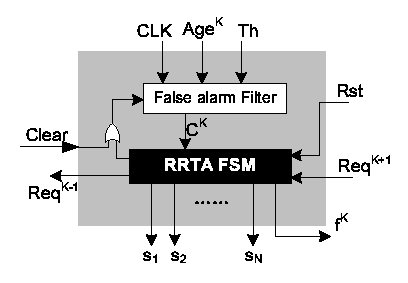
\includegraphics[width=0.5\textwidth]{fig2-20.eps}%{agent.eps}
   \caption{Adaptation agent}\label{agent}
\end{figure}

Figure \ref{agent} shows the top view of an agent architecture. The agent can send a request $Req^{K-1}$ to an agent in the $(K-1)$st stage to enable forward adaptation for the $K$th stage logics, and can also receive $Req^{K+1}$ coming from an agent in the $(K+1)$st stage to enable forward adaptation for the $(K+1)$st stage logics. A failure signal ($f^K$) is asserted if an aging alarm still appears after the agent has traveled the all adaptation states.

Each agent consists of a RRTA unit and a False Alarm Filter; the RRTA is a finite state machine (FSM), and the filter is a counter. Signal $Age^K$, which is an aging alarm signal coming from an aging sensor, is cycle-updated. The adaptation process, however, should not be triggered at the same pace, otherwise it could incur useless adaptations due to the presence of \emph{false alarms}.

\subsubsection{False Alarm Filter}
The false alarms are caused by subtle dynamic variations \cite{degradation_05} such as power noise, temperature fluctuation. But aging can still be reliably detected even in the presence of these dynamic variations. The main reason is that the locations of aged paths generally won't change over time. This is very different from the power noise which mainly results from the time-varying current demand and exhibits much randomness in both spatial and temporary dimensions. Hence, the aging alarms traced back to the same spots are more "repetitive", by contrast to the more random dynamic variations. By exploiting the repetitiveness, we can filter the most, if not all, false alarms.

Identifying the ``repetitiveness" can be realized with a counter, which records the number of alarms in a specified span of time.  A confident aging alarm ($C^K$) is asserted only when corresponding counter reaches a threshold ($Th$) that has been calibrated according to some alarm statistics. To eliminate the aggregate effect of these false alarms, after each period of trial adaptation, the counter should be cleared.

Figure \ref{synadp} exemplifies the change of a filter counter over time. The normal perturbations (false alarms) have little chance to trigger adaptations; two adaption trials are conducted: the first fails, thus the counter still keeps growing after the invalid adaptation, while the second succeeds and the counter does not increase any more.

\begin{figure}[t]
\centering
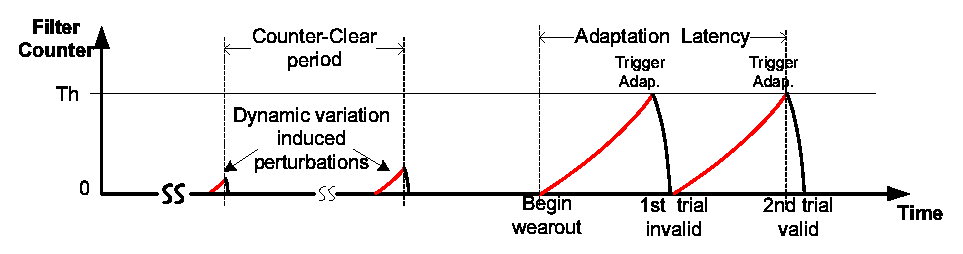
\includegraphics[width=0.85\textwidth]{fig2-21.eps}%{cnt.eps}
   \caption{Example of filter counter change}\label{synadp}
\end{figure}


\subsubsection{Complexity Analysis and Two Critical Optimizations}\label{section_complexity} In Example \ref{rrtaexample}, for agent $A_K$ handling 7-bit clock-steering signals (3 bit for BAFFs and 4 bit for FAFFs), there are up to 22 ($2^3-1+2^4-1$) candidate states. Furthermore, each agent owns a private filter, which could incur non-negligible area overhead. Fortunately, with the following two optimizations the potential complexity can be decreased significantly.

Many adaptation state candidates can be removed with little loss of adaptability. The following shows how to use "logic cones" analysis to

1) remove those low-effective states for loose-couple logic cones, or

2) merge them for tight-couple logic cones.

\exmp Figure \ref{logiccone} exemplifies a stage of logic covered in two logic cones without overlap---loose-couple, referred to case (a) and with some overlap---tight-couple , referred to case (b). Suppose that flip-flop F1, F2, F3, and F4 are FAFFs and F5, F6 are BAFFs.

For case (a), the basic adaption states for F5 and F6 are \{01, 10, 11\}. Clearly, the state "11" is effective only in the case: (at least) one aged path in each logic cone causes aging alarm at the same time. Such ``coincidence", however, hardly happens; thus, we can safely remove the "11" from the adaptation state candidates. Similarly, the forward adaption states (for F1, F2, F3, F4) can be simplified from \{0001, 0010, $\ldots$, 1111\} to \{0001, 0010, 0100, 1000, 0011, 1100\}.

For case (b), the overlap can reduce some efficiency of such optimization. Removing state "11" for F5 and F6 may be problematic since an aging alarm could be raised at F5 and F6 simultaneously if aging happens in the overlap zone. For the same reason, the forward adaptation states should not be removed. However, since these two logic cones is tightly coupled, using 1-bit state for F5 and F6 should be reasonable. Then the backward adaptation states can be reduced from \{01, 10, 11\} to \{1\} . Similarly, the forward adaptation states can be simplified to \{001, 010, 100, 011, 110, 111\} (for F1, $<$F2,\,F3$>$, F4).


\begin{figure}[t]
\centering
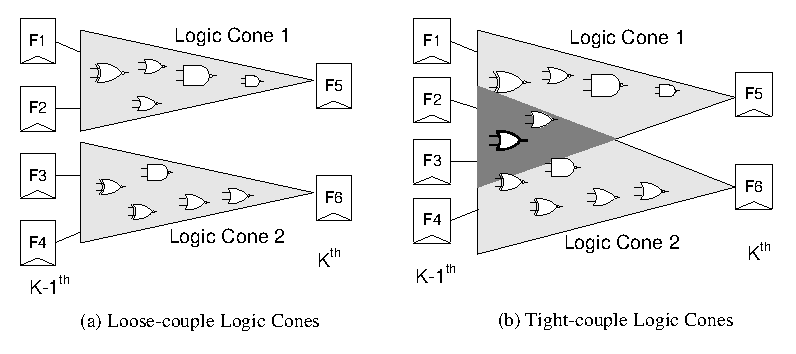
\includegraphics[width=0.85\textwidth]{fig2-22.eps}%{logiccone2.eps}
   \caption{Logic cones}\label{logiccone}
\end{figure}

Each agent owning a private false-alarm filter is cost-inefficient, since such private filter is only necessary in such case: all the agents are active at the same time---that is a quite small probability event. Enabling filter sharing  can be readily implemented by appending selection-indicating bits $S$ to original filter. Figure \ref{agent_share} shows an example of two agents sharing one filter.

\begin{figure}[t]
\centering
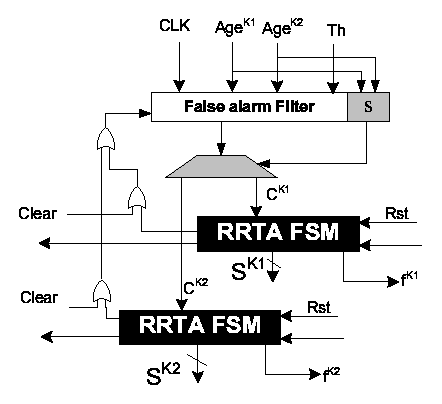
\includegraphics[width=0.65\textwidth]{fig2-23.eps}%{agent_share.eps}
   \caption{Two agents share one false alarm filter}\label{agent_share}
\end{figure}


The above have described the individual agent design and functionality; the following will detail how to deploy the agents and corresponding sensors with respect to the correspondence of BAFFs, FAFFs, and UAFFs.

\subsubsection{Deploy Agents and Sensors}\label{deploy_agentsensor}
\begin{figure}[t]
\centering
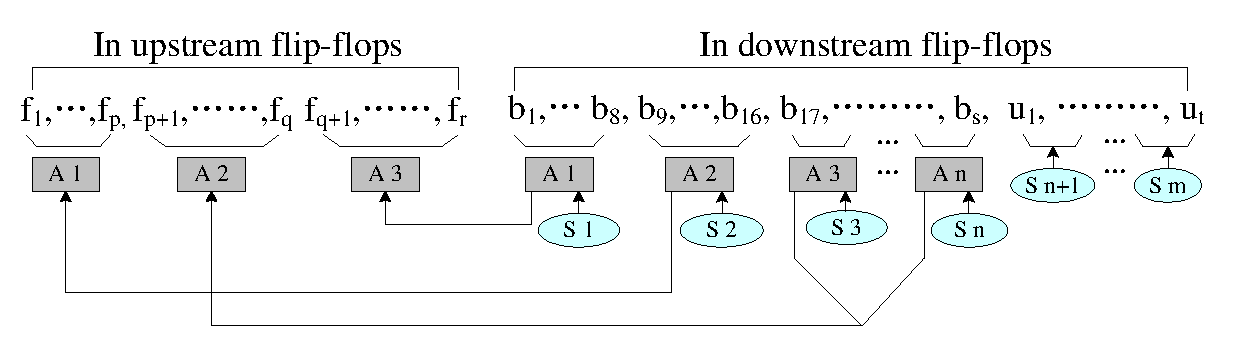
\includegraphics[width=0.85\textwidth]{fig2-24.eps}%{deploy2.eps}
   \caption{Deploying sensors and agents}\label{delpoy}
\end{figure}

Suppose that the $K$th stage with downstream flip-flops $$FF_{k}=\{f_1^{k}, \ldots,\; b_1^{k}, \ldots, b_s^{k}, \;u_1^{k}, \ldots, u_t^{k}, \;g_1^k, \ldots \}, $$ and upstream flip-flops $$FF_{k-1}=\{f_1^{k-1}, \ldots,  f_r^{k-1},\; b_1^{k-1}, \ldots, \;u_1^{k-1}, \ldots, \;g_1^{k-1}, \ldots \}.$$ Among these flip-flops, only $\{b_1^{k}$, $\ldots$, $b_s^{k}\}$ and $\{f_1^{k-1}$, $\ldots$, $f_r^{k-1}\}$ can contribute to the adaptation in the $K$th stage. We explain the policy of
deployment with the following example:

Figure \ref{delpoy} shows the $K$th stage's upstream and downstream flip-flops that can contribute to adaptation, and each sensor is assumed to handle eight signals at the most. Sensor $S_1$, $\ldots$, $S_n$ are assigned to $b_1$, $\ldots$, $b_s$, and $S_{n+1}$, $\ldots$, $S_m$ to $u_1,\ldots, u_t$. Furthermore, suppose that the upstream flip-flops can be divided into three loose-couple groups: $f_1,\ldots, f_p$ are relevant inputs to $b_9, \ldots, b_{16}$, $f_{p+1},\ldots, f_q$ to $b_{17}, \ldots, b_s$, and $f_{q+1},\ldots, f_r$ to $b_1, \ldots, b_8$. Three polices can be used to guide the deployment:

1) The agents are not required for the UAFFs, e.g. $u_1, \ldots, u_t$; but sensors is required,
i.e. $S_{n+1}$, $\ldots$, $S_m$.

2) The agents assigned to FAFFs, unlike that assigned to BAFFs, are triggered by the downstream agents, rather than by any sensors (so false alarm filters are not necessary for the FAFFs' agents).

3) The connecting relations between upstream agents and downstream agents is determined by the target circuit topology which can be obtained by conducting logic cones analysis (the ultimate goal of using logic cones analysis for ReviveNet is to extract all loose-couple logic cones, and merging all tight-coupling logic cones).

The number of required sensors $N_{sensor}$ for the $K$th stage is
\begin{equation}\label{numsensor}
N_{sensor}=\frac{s}{BW_{sensor}},
\end{equation}
where $BW_{sensor}$ denotes the maximum number of nodes that each sensor can handle.

The number of required agents $N_{agent}$ is
\begin{equation}\label{numagent}
N_{agent}=N_{agent}^{dn}+N_{agent}^{up},
\end{equation}
where $N_{agent}^{dn}$ denotes the number of downstream agents and $N_{agent}^{up}$ denotes that of upstream agents. Generally, each downstream agent is assigned a sensor and has the same bandwidth with the associated sensor, so \begin{equation}N_{agent}^{dn}=N_{sensor}\end{equation}. The number of upstream agents and its' bandwidth, however, is circuit topology-specific; thus the area of each upstream agents are not constant. For instance, the upstream A1, A2, and A3 in Figure \ref{delpoy} may handle different number of FAFFs (different bandwidth).

\begin{figure*}[t]
\centering
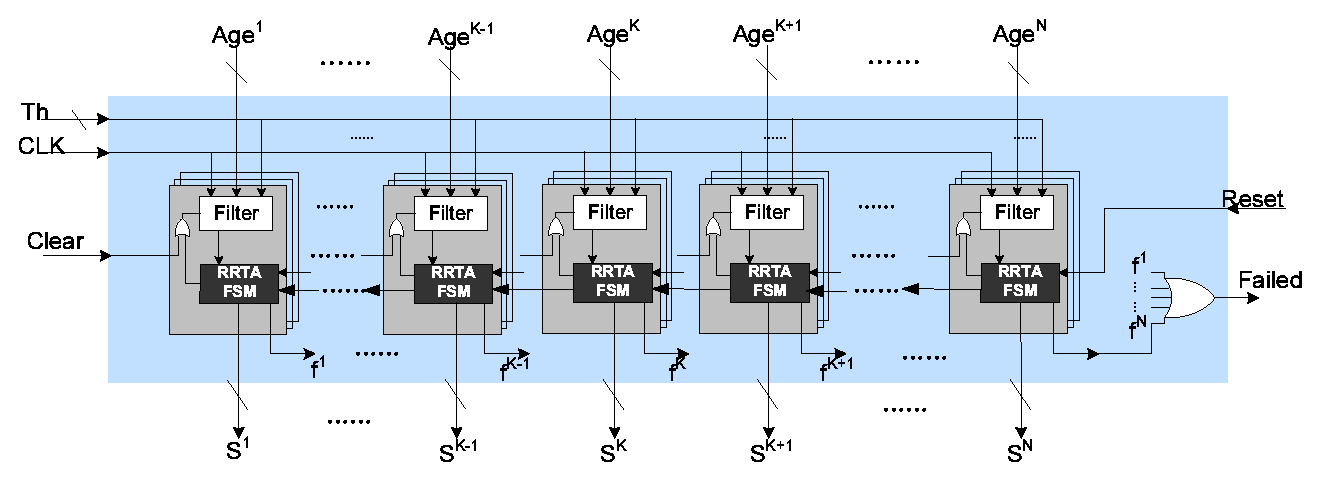
\includegraphics[width=0.95\textwidth]{fig2-25.eps}%{agent_set.eps}
\vspace{-0.2cm}
   \caption{A group of synergistic agents for a n-stage pipeline}\label{sac}
\end{figure*}


Base on the above analysis, we present a typical organization of agents for a N-stage pipeline in Figure \ref{sac} (no filter sharing illustrated for simplicity), where $Age^K$ is a set of aging alarm signals from the $K^{th}$ stage and $S^K$ is a set of clock-steering signals to enable localized adaptations.

\subsection{Architecture Implementation}\label{imple_issue}

\subsubsection{Clock Generation and Overhead Analysis}\label{section_clcokgen}

ReviveNet needs two extra clocks, FCLK and BCLK, with intentional skew from CLK. These clocks can be generated by using a DLL(delay-locked loop). DLLs are widely used to reduce the clock skew across clock domains \cite{clock_01} \cite{DLL_00} \cite{DLL2_04}. The detailed design of a DLL is beyond the scope of this paper. A major concern is whether those PVT (process, voltage, and temperature) variations can spoil the intentional skew. Fortunately, many industry practices have shown that implementing clocks with only picoseconds of skew is very practical. For example, even in conventional tree-based clock networks across 500$mm^2$ processor die with frequency up to 2.5GHz , the unintended clock skew can be efficiently limited less than 10ps \cite{Itanium_clock05}. Thus, it can be extrapolated that for relatively spatial concentrated pipeline logics with less die area, the unintentional skew can be further optimized. In fact, even "10ps" is generally one order of magnitude smaller than the intentional skew. Moreover, the power consumption of a processor's DLLs, commonly, is less than 2\% \cite{clockpower_02}, and the hardware overhead is very limited. Hence, with the state-of-the-art clocking techniques, we believe that generating the adaptation clocks won't be a major obstacle.

In our scheme, we point out that although ReviveNet needs two extra clocks, our evaluation results show that on average the load of each of them is only about 20\% of CLK's. This is because only BAFFs and FAFFs need to be deployed with extra clocks, while the proportion of the two types of flip-flops takes only about 19\%. That means more than 80\% clock distributions are kept intact. This implies that 1) the clock power will not be tripled  but far less than that (section \ref{section_results}), and 2) the routing complexity will not be significantly increased. So, the overall design complexity should be in check.

\subsubsection{ReviveNet-supported Clock Gating}\label{section_clockgate}
\begin{figure}[t]
\centering
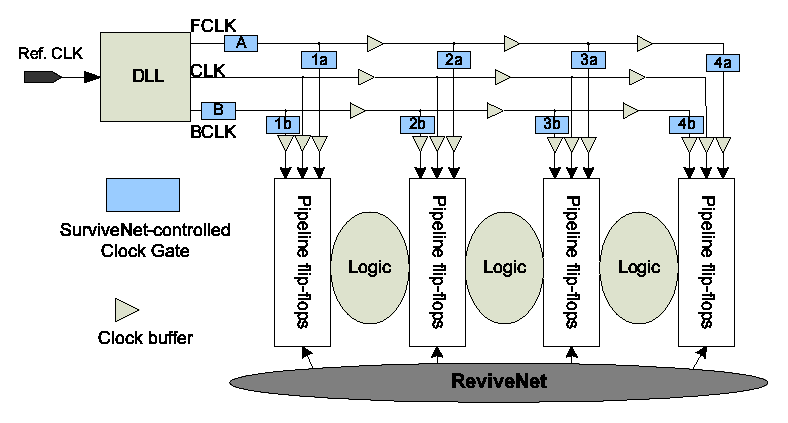
\includegraphics[width=0.7\textwidth]{fig2-26.eps}%{clkgate.eps}
   \caption{ReviveNet-supported clock gating}\label{clkgate}
\end{figure}

Since aging adaptations usually are conducted on minority aging-prominent logics, so for the rest logics, It's better to keep the associated standby clocks off.

ReviveNet can readily support a high-efficient clock gating to further reduce the extra power consumed by the additional FCLK and BCLK. Figure \ref{clkgate} shows ReviveNet's clock network. The basic clock routing for CLK can be found in \cite{clockpower_02}. Usually, the pipeline will not suffer from aging in the early phase of lifetime, so FCLK and BCLK do not need to be enabled during that period. Two "root" clock gates, A and B, are employed to totally cut FLCK and BCLK off the DLL; thereby no power is consumed on the extra clock networks. If some parts of the pipeline need to be adapted, the corresponding root gate and branch gate can be switched on on-demand, while the unrelated clock branches are still kept off.

\subsubsection{Implication of Multi-cycle Paths}
Since a multi-cycle path usually consist more logic gates, the timing margin that a single-cycle path is able to share is likely to be inadequate. For example, suppose the cycle period is 1ns, for a 5-cycle path with fresh path delay 4.7ns. Then 10\% degradation yields 5.17ns ($4.7+4.7\times10\%$), which must violate the 5-cycle path timing requirement. But a single-cycle path can only contribute 0.075ns (1$\times$15\%/2) slack (suppose $TH$=0.15). Hence, although this slack, if exploited, can partially alleviate the aging delay, we had better not rely on single-cycle paths to salvage multi-cycle paths.

For multi-cycle paths, especially for "many-cycle" paths, we think a more effective way is to resort to some logic optimizations. For example, re-organize the 5-cycle paths into 6-cycle paths, to naturally gain more aging tolerability, though this approach usually needs to interact with some microarchitecture implications (which are supposed to beyond the scope of this paper).

\subsubsection{Impact of ReviveNet Wearout}\label{section_impactwearout}
Aging can indeed affect all logics on the chip, including aging sensors, adaptation agents, and even clocks networks.
	
Among them, the adaptation agents are relatively timing-non-critical; the latency of each adaptation, for example, increase from 1 cycle to 2 cycles should not be critical for an effective adaptation. This implies that, to protect these agents from the impact of aging, we can "over-design" the agents; that is to reserve conservative timing margins for these agents. For the clock networks, aging may results skew drift. Since skew-controlling actually is one of the primary objectives in many traditional clock optimizations, and we suppose that is beyond the scope of this paper. The sensor degradation, however, can impair the effectiveness of the proposed ReviveNet; after all, we cannot count on the adaptations triggered by unreliable sensors.
	
Fortunately, because the sensors' area and power overhead are small ($<$5\% and 1\%, respectively), so we can also over-design those sensors by using such as transistor-sizing techniques \cite{Temporal-Performance-Degradation-date06}. Usually, transistor-sizing impose about 9\% area overhead \cite{Temporal-Performance-Degradation-date06}, the overall extra overhead, therefore, should be very small.


\subsection {Modele Based Reliability Analysis}\label{section_model}

\subsubsection{Reliability Model}
Commonly, the reliability of semiconductor is modeled with Weibull distribution \cite{Handbook}. Given a circuit, the reliability at  time $t$ is given by
\begin{equation}\label{weibull}
  R(t)=\mbox{exp}[-(\frac{t}{\alpha})^\beta]
\end{equation}
where $\alpha$ is the characteristic time-to-failure and $\beta$ is the shape parameter \cite{Handbook}. The MTTF is calculated by
\begin{equation}
MTTF=\int^\infty_0 R(t)\,\mbox{d}t.
\end{equation}

Suppose that there are $n$ critical paths in the target circuits. The reliability of the $i$th path at time $t$ can be expressed as
\begin{equation}
  R_i(t)=P(T_i(t)<T)
\end{equation}

where, $T_i(t)$ denotes the delay of the $i$th path at time $t$; $T$ is the clock cycle period. Let's further assume that these paths are independent to each other, as Bowman et al. assumed in \cite{variation_jssc02}. Then, $R(t)$ can be put in another way:

\begin{equation}\label{anotherway}
  R(t)=\prod^n_{i=1} R_i(t)=\prod^n_{i=1} P(T_i(t)<T).
\end{equation}

Moreover, we treat each critical path as a "mini-component", then $R_i(t)$ can be expressed as
\begin{equation}
  R_i(t)=P(T_i(t)<T)=\mbox{exp}[-(\frac{t}{\alpha_i})^{\beta_i}],
\end{equation}
then we have
\begin{equation}
  R(t)=\prod^n_{i=1}
  \mbox{exp}[-(\frac{t}{\alpha_i})^{\beta_i}]=\mbox{exp}[-\sum^n_{i=1}(\frac{t}{\alpha_i})^{\beta_i}].
\end{equation}
The corresponding MTTF can be calculated by
\begin{equation}\label{mttf}
  MTTF=\int^{\infty}_{0} \mbox{exp}[-\sum^n_{i=1}(\frac{t}{\alpha_i})^{\beta_i}]\,\mbox{d}t.
\end{equation}

The above general analysis has not taken the effect of ReviveNet into account yet, and the following will involve it. When considering ReviveNet, the group of $\mathcal{R}=\{$$R_1(t)$, $R_2(t)$,$\ldots$, $R_n(t)\}$ can be divided into three groups according to the adaptability of each critical path:
\begin{itemize}
  \item Group 1: the set of critical paths in case 2) and 3) (Section 3.1) which can only be backward or forward adapted by $TH/2$;
  \item Group 2: the set of critical paths in case 1) which can not only be backward, but also forward adapted by $(TH/2+TH/2)=TH$;
  \item Group 3: the set of critical paths in case 4) which are unadaptable.
\end{itemize}

 Suppose that there are $l$ paths in Group 1, $m$ paths in Group 2, and the other $(n-l-m)$ in Group 3. Without  loss of generality, denote the first group as $\mathcal{R}_{u}=\{R_1(t), R_2(t),\ldots, R_l(t)\}$, the second group as $\mathcal{R}_{b}=\{R_{l+1}(t), \ldots, R_{l+m}(t)\}$, and the third group as $\mathcal{R}_{n}=\{R_{l+m+1}(t), \ldots, R_{n}(t)\}$. Then we have the ReviveNet-involved reliability term $\widetilde{R}_i(t)$, as follows:

\begin{equation}\label{new_term}
{\small
 \widetilde{R}_i(t)=\left\{
\begin{array}{ll}
P(T_i(t)<T+{TH}/{2}) & \mbox{if $i=1, 2, \ldots, l$,} \\
P(T_i(t)<T+ TH) & \mbox{if $i=l+1, \ldots, l+m$,} \\
P(T_i(t)<T) & \mbox{if $i=l+m+1, \ldots, n$.}
\end{array} \right.}
\end{equation}

The enhanced MTTF can be obtained:
\begin{equation}\label{mttfr}
MTTF_R = \int^\infty_0  \prod^n_{i=1} \widetilde{R}_i(t) \,\mbox{d}t.
\end{equation}

We define a relative MTTF improvement, $EX$ (short for "EXtension of lifetime"),  denoted by
\begin{equation}
  EX=\frac{MTTF_R}{MTTF}
\end{equation}
to evaluate the effect of ReviveNet.

To calculate $EX$ we have to figure out the relations: $\alpha_i=\alpha_i(T)$, and $\beta_i=\beta_i(T)$. Figure \ref{weibull} shows the qualitative relations; the following describes how to figure out the two relations.

In weibull distribution,
\begin{equation}\label{ab}
\beta=\frac{1.38}{\mbox{ln}(t_{50}/t_{16})},\;\mbox{ and }\; \alpha =
\frac{t_{50}}{ln(2)^{1/\beta}}\approx t_{63}
\end{equation}
where $t_x$ means the lifetime at the failure rate $x\%$ \cite{Handbook}, as shown in Figure \ref{weibull}. Intuitively, given a critical path, if more margin is reserved for it, then the wearout should be also postponed, as curve I and II show. ReviveNet can provide margin for some critical paths, thereby postponing the onset of wearout. In the following, relying on the assumption: the curve I and II are same in "shape", can greatly simplify the discussion, although the actual failure rate in the wearout region for I and II may slightly differ from each other.

Figure \ref{weibull} also reveals the effect of ReviveNet for a specific critical path can be reflected by the parameter $\alpha$ and $\beta$. Let $t_{50}= t_{16}+\Delta$, and commonly, $\Delta
\ll t_{16}$ then
\begin{equation}
  \beta=\frac{1.38}{\mbox{ln}(1+\Delta/t_{16})} \approx \frac{1.38}{\Delta/t_{16}}
\end{equation}

For the both curves, because $\Delta_I=\Delta_{II}$, so
\begin{equation}\label{frac}
\frac{\beta_I}{\beta_{II}}=
\frac{t_{16,I}}{t_{16,II}},\;\;\frac{\alpha_I}{\alpha_{II}}=\frac{t_{63,I}}{t_{63,II}}
\end{equation}


\begin{figure}[t]
\centering
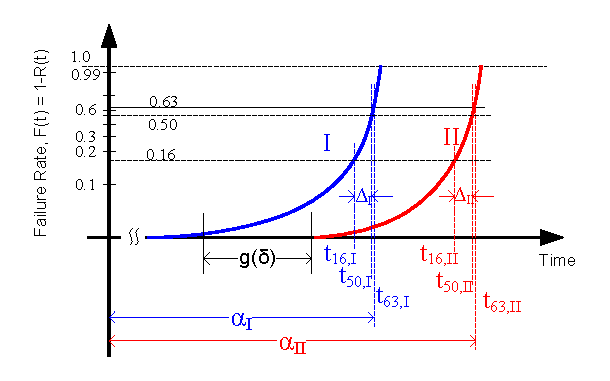
\includegraphics[width=0.7\textwidth]{fig2-27.eps}%{weibull2.eps}
\vspace{-0.2cm}
   \caption{Weibull failure rate in wearout period}\label{weibull}
\end{figure}

Furthermore, let
\begin{equation}\label{newab}
t_{16,II}=t_{16,I}+g(\delta) \mbox{ and }  t_{63,II}=t_{63,I}+g(\delta)
\end{equation}

where $g(\delta)$ denotes the lifetime extension contributed by tolerating $\delta$ aging delay; $\delta$ can be $0$, $TH/2$, or $TH$, determined by the specific adaptability of paths. Clearly, function $g(\delta)$ is highly dependent to specific aging mechanisms. Unfortunately, no such function proposed so far that can accurately reflect the performance degradation over time under a variety of aging mechanisms (some of them such as dielectric breakdown even have not been well-understood by the community \cite{Reliability_limits_IBM02}). In the following case study, we just use the relatively well-studied NBTI, one of the major reliability challenge, as target aging mechanism to evaluate the ReviveNet. We expect the physical community to contribute a much more versatile $g(\delta)$ in the near future.

Paul. et al. proposed a NBTI circuit delay model that capture the relation ship between the threshold voltage change and resultant delay degradation \cite{NBTI_Impact05}: the NBTI degradation is much fast at the early years, and then slowed down later, as the trend shown in Figure \ref{nbti}. Moreover, Figure \ref{nbti} also shows the relation between $\delta$ and $g$; we obtain $g(\delta)$ by regressing the results in \cite{Impact-of-NBTI_07}. More details are presented in Section 7.2.


\subsubsection{Implication of $TH$}
Eq. (\ref{new_term}) implies an essential tradeoff behind ReviveNet. Note that the critical paths in Group 3 is free from ReviveNet; only the Group 1 and Group 2 can contribute to the lifetime improvement. However, given a target circuits, the sizes of the three groups are depends on the $TH$: on one hand, larger $TH$ can result higher percentage of of UAFFs, and thereby more critical paths in Group 3, and thus leads to fewer adaptable critical paths; on the other, the larger $TH$ implies that more aggressive tolerability to aging delay on those adaptable critical paths. Hence, given a circuit, there should be an optimum $TH$ that can maximize the $EX$.


\begin{figure}[t]
\centering
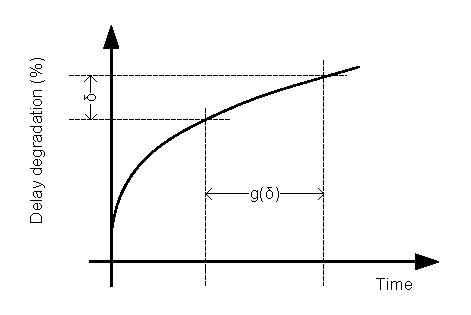
\includegraphics[width=0.5\textwidth]{fig2-28.eps}%{nbti2.eps}
\vspace{-0.3cm}
   \caption{NBTI degradation}\label{nbti}
\end{figure}

\subsection{Case Study and Discussion}\label{section_casestudy}
\subsubsection{Experiment Setups}
We took a fully pipelined FPU \cite{OpenSPARC_06} as our target circuit which implements the SPARC V9 floating-point instructions and supports all IEEE 754 floating-point data types. The FPU comprises three independent pipelines: Multiplier pipeline (MUL), Adder pipeline (ADD) and Divider pipeline (DIV). In this paper, we used the largest MUL, which takes up to 50\% area of the FPU, as the target pipeline. More design details can be found in \cite{OpenSPARC_06}.

The FPU was synthesized using Design Compiler with UMC
0.18um technology. We set the performance as the synthesizing priority to smooth the distribution
of path delay as much as possible. Then, the path delay was analyzed with PrimeTime.

First, we identify the adaptability of each pipeline flip-flop, based on the STA results. Then, the
deployment of sensors and agents can be determined as follows: for each flip-flops $i$, find the
upstream flip-flops that in the same logic cone; this can be done by matching the start points of
paths ended with the flip-flop $i$. The number of required sensors and agents can be figured out by
using Eq.(\ref{numsensor}) and Eq.(\ref{numagent}).
Then, we evaluate the MTTF improvement ($EX$) by using the proposed reliability model.
Finally, we present the overhead in terms of area, power, and performance.

\subsubsection{Results and Discussions}\label{section_results}

\begin{figure*}[t]
\centering \subfigure[\small{Skew variation: 1\%}]
%{\includegraphics[width=0.34\textwidth]{EX2_1percent.eps}} \hspace{-0.5cm}
{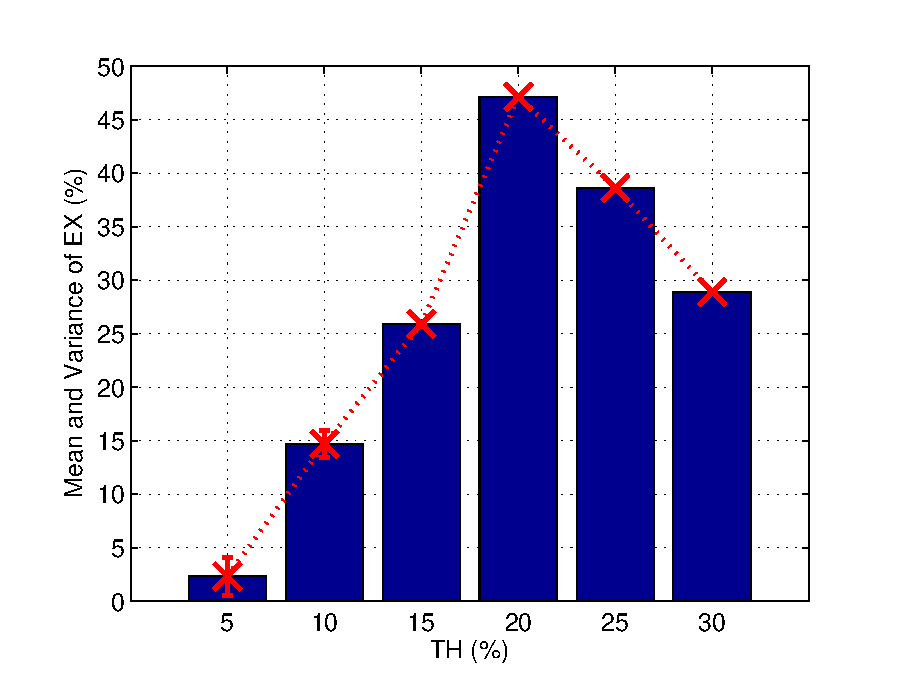
\includegraphics[width=0.34\textwidth]{fig2-29a.eps}} \hspace{-0.5cm}
\subfigure[\small{Skew variation: 3\%}]
%{\includegraphics[width=0.34\textwidth]{EX2_3percent.eps}}\hspace{-0.5cm}
{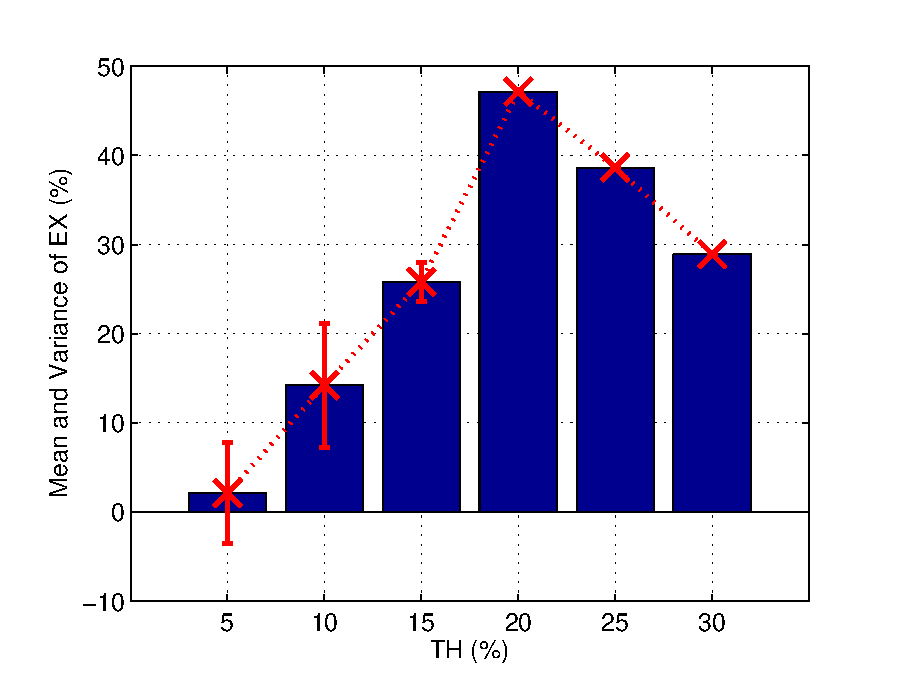
\includegraphics[width=0.34\textwidth]{fig2-29b.eps}}\hspace{-0.5cm}
\subfigure[\small{Skew variation: 5\%}]
%{\includegraphics[width=0.34\textwidth]{EX2_5percent.eps}} \vspace{-0.2cm}
{\includegraphics[width=0.34\textwidth]{fig2-29c.eps}} \vspace{-0.2cm}
\caption{MTTF improvement at different $TH$ and clock skew variations}\label{ex}
\end{figure*}

\textbf{Lifetime Improvement Analysis:} We conduct the lifetime evaluation based on the 65nm technology (the STA results actually are based
on a 180nm technology due to lack of 65nm compiler libraries. To match the following analysis, we
scale the STA results to 65nm based on scaling theory \cite{JMRabaey}). The NBTI degradation
results are from \cite{Impact-of-NBTI_07}. The lifetime is studied at different configurations:
without ReviveNet, and with ReviveNet, at $TH$=5\% (of the delay of the most critical path), 10\%,
15\%, 20\%, 25\%, 30\%, respectively. The necessary $g(\delta)$ at these $TH$ is as follows:
\begin{equation}\label{reg}{\small
\begin{array}{ll}
g(0.05)=876 \mbox{(hours)}; &g(0.1)=8,760 \mbox{(hours)};\\
g(0.15)=21,900 \mbox{(hours)};& g(0.2)=43,800 \mbox{(hours)};\\
g(0.25)=87,600 \mbox{(hours)};& g(0.3)=131,400 \mbox{(hours)}.
\end{array}}
\end{equation}

For example, $g(0.05)=876$ (hours) means that the 5\% tolerability to delay degradation can
translate to 876 hours lifetime extension. The above results faithfully reflect that NBTI
degradation which is much faster at the early years and slowed down over time.

Next, the weibull parameter $\alpha$ and $\beta$ is calculated as follows: we use empirical data:
$t_{16}=35,040$hours (4 years) and $t_{63}=39,420$hours (4.5 year) (thus $\Delta=4380$ hours).
Then, from Eq.(\ref{ab}), we have the original $\alpha$ and $\beta$ for a critical path is
$\alpha=39,420 \mbox{ (hours)}, \beta=11.04$.
Then, combined Eq.(\ref{reg}) with Eq.(\ref{newab}) and then put it into Eq.(\ref{frac}), the new
$\alpha$ and $\beta$ at different $TH$ can be obtained. When calculating MTTF, we
assume that the critical paths with the same adaptability have the same $\alpha$ and $\beta$.

Finally, base on the STA results, the three path groups $\mathcal{R}_u$, $\mathcal{R}_b$, and
$\mathcal{R}_n$ at different $TH$ configurations can be determined, respectively.

With the above preparation, the original and improved MTTF can be calculated with Eq.(\ref{mttf})
and Eq.(\ref{mttfr}); Figure \ref{ex} shows the detailed results that offer a significant insight: larger $TH$ does not necessarily results higher improvement in lifetime reliability.
The underling reason is on one hand larger $TH$ can facilitate more aggressive timing stealing, thereby
improving more reliability for adaptable paths; on the other, larger $TH$ will definitely results
more UAFFs and thereby more unadaptable paths. In other words, the overall MTTF is determined not
only the reliability benefit of individual path, but also the population of paths governed by
ReviveNet. At the optimum configuration, $TH$=20\%, MTTF can be improved by 48.7\%.

\textbf{Impact of Clock Skew Variation:} The effectiveness of ReviveNet, as concerned in Section \ref{section_clcokgen}, is also impacted by the variation in clock skew (measured by $skew/cycle\_period$ in this paper). The impact actually results in corresponding variation in ``effective" $TH$. We find that the degradation can only be marginally impacted if the adaptation clocks are kept beyond a large interval, say, $TH>0.2$. Specifically, Figure \ref{ex}(a), (b), and (c) show the $EX$ variation under different clock skew variations: 1\%, 3\%, and 5\%, respectively. Two trends can be clearly identified: i) the degradation in effectiveness  reduces with  $TH$ increasing, and ii) the larger clock skew variation results in more variation in MTTF improvement. Hence, the worst-case efficacy under overly ``weak" adaptation intensity, i.e. $TH<0.1$, can be significantly reduced under 3\% skew variation, and even totally diminished under 5\% skew variation, as shown in Figure \ref{ex}(b) and (c). However, the optimal design point is around $TH=0.2$ where the impact of clock skew is marginal.

In addition, it is practical to keep the clock skew below 3\% by using the state-of-the-art clocking techniques (for example, 10ps skew variation for 2.5GHz Itanium processor \cite{Itanium_clock05}). This can further justify the effectiveness of ReviveNet.



\textbf{Overhead Analysis:} We evaluate ReviveNet's overhead from three aspects: silicon area, power, and performance. The
overhead largely depends on the parameter $TH$ (section 7.2).

\smallskip
\noindent{\bf 1. Area Overhead.}

{\bf Sensor Configuration:} The number of sensors for each stage depends on specific sensor design
\cite{failure_prediction_07}\cite{SVFD_09};

we take the configuration of one sensor handles eight signals.



{\bf Agent Configuration:} Agents are configured as follows: 6-bit False Alarm Filter which can
filter as much as 64 false alarms during one adaptation period. We study the area overhead with
different degrees of Filter sharing: no sharing, two agents sharing one filter, four agents sharing
one filter, and eight agents sharing one filter.



The sensor and agents are insert into the original MUL netlist, and re-synthesized using the same
technology. Figure \ref{totalarea} shows the overall area overhead under different configurations. Generally, the area overhead is small: only 9.5\% at the recommended $TH$=0.2.

\begin{figure}[t]
\centering
\includegraphics[width=0.6\textwidth]{fig2-30.eps}%{areaoverhead.eps}
\vspace{-0.3cm}
   \caption{Area overhead with different sharing configurations}\label{totalarea}
\end{figure}


\smallskip \noindent{\bf 2. Power Overhead.}

Power overhead mainly comes from ReviveNet logics (sensors and agents) and extra clock networks.
That is
$$P_{overhead}=P_{logic}+P_{clk}=(P_{sensor}+P_{agent})+P_{clk}.$$ The following results show that
$P_{logic}$ is negligible, and the major power overhead results from $P_{clk}$.

{\bf 1) Logic Power.} We use PrimePower to evaluate $P_{logic}$. Evaluation results
show that even in the worst case\,---\,each sensor raises an aging alarm in every cycle\,---\,the
power overhead caused by the sensors and agents is negligible. Figure \ref{logicpower} shows that a
typical logic power overhead ($TH=0.2$) is less than 5\%.


{\bf 2) Clock Power.} The worst case overhead of clock power, $P_{clk}$, is more significant than that
of logics. In ReviveNet, the clock power can be calculated as
$$P_{clkall}=P_{pipeffs} + P_{DLL} + P_{buf} + P_{wire}+ P_{mux} \, \mbox{\cite{clockpower_02}} $$ where
$P_{pipeffs}$ and $P_{DLL}$ is the power consumed by pipeline flip-flops and DLL, and $P_{buf}$,
$P_{wire}$, and $P_{mux}$, are power consumed by  clock buffers (drivers), clock wires, and clock
multiplexers, respectively. $P_{pipeffs}$ and $P_{DLL}$ stay unchanged because little modifications
are made to them. The clock buffers which take the most proportion, 56\%,  in the original
pipelines, increase by 32\% to support FCLK and BCLK networks (the increase in buffers is
proportion to the increase in clock load). $P_{wire}$ almost triples, but it takes only about 10\%
in original pipelines. Compared with the other proportions, $P_{mux}$ is ignorable. Overall, the
clock power increases by 38\%.

The previous study \cite{clockpower_02} shows generally for a pipelined processor,
the clock power is about the 30$\backsim$40\% (denoted by $\eta$) of the total power,
so this increase contribute to the overall power overhead is calculate by
$$[(1-\eta) + \eta \times (1+38\%)] - 100\%.$$
Since $\eta$ is about 30$\backsim$40\%, the overall overhead should be between 11.4$\backsim$15.2\%.

Note that this overall power overhead is in the \emph{Worst Case}---all the drivers of FCLK and BCLK
are turned on. However, little power overhead is imposed in the early period of lifetime, because
few of the extra logics and clock networks need to be turned on due to  little appreciable aging
delay. Moreover, we believe with ReviveNet-supported clock gating, the overall power
overhead can be significantly reduced even after the onset of wearout.



\smallskip \noindent{\bf 3. Performance Overhead.}

ReviveNet needs some sensors. From circuit design perspective, these sensors can cause some
capacitance load to the target pipelines. This concern, however, will not be substantial because
the performance penalty imposed by such capacitance load is less than 1\%
\cite{failure_prediction_07}\cite{SVFD_09}.


\begin{figure}[t]
\centering
\includegraphics[width=0.5\textwidth]{fig2-31.eps}%{poweroverhead_workmode.eps}
\vspace{-0.3cm}
   \caption{Power overhead of sensors and agents in working mode}\label{logicpower}
\end{figure}

ReviveNet improves the lifetime reliability only by tolerating the aging delay, which may not be
comprehensively enough. In addition, ReviveNet does not suppose to handle some "abrupt" wearout
which in reality is possible due to some mechanical stress induced failures.
In addition, ReviveNet is not designed for coping with all corner cases, but for average case;
in other words, ReviveNet is statistically effective, rather than deterministic.

\section{Summary}
The proposed ReviveNet architecture, without compromising with the nominal architectural
performance, can efficiently hide the aging induced delay, thereby improving the lifetime
reliability. The weakest links of lifetime can be locally and efficiently remedied by enabling a
path-grained adaptation mechanism; ReviveNet employs a group of collaborative cost-efficient agents
to achieve this purpose. A new reliability model is also proposed to quantitatively evaluate the
effect of ReviveNet. Evaluation results based on a case study show that the ReviveNet can improve
the MTTF by 48.7\%, at the expense of about 9.5\% area overhead, and about 4.9\% power increase during aging-free period.

\bibliographystyle{plain}
\bibliography{refs}
